\newif\iftalk
\talktrue

\documentclass[oneside]{book}
\usepackage{graphicx}
\usepackage{natbib}
\usepackage{amsfonts}
\usepackage{amssymb}
\usepackage{amsthm}
\usepackage{bm}
\usepackage{Sweave}
\usepackage{lscape}
\usepackage{tocbibind}
\usepackage{makeidx}
\usepackage{color}
\usepackage{hyperref}

\let\proglang=\textsf
\newcommand{\pkg}[1]{{\fontseries{b}\selectfont #1}}
  \hypersetup{%
    hyperindex = {true},
    colorlinks = {true},
    linktocpage = {true},
    plainpages = {false},
    linkcolor = {blue},
    citecolor = {blue},
    urlcolor = {red},
    pdfstartview = {Fit},
    pdfpagemode = {UseOutlines},
    pdfview = {XYZ null null null}
  }

\makeindex

%\SweaveOpts{width=60}
% \VignetteIndexEntry{MCMCglmm CourseNotes}
%\newcommand{\begin{document}}{\chapter{}}
%\newcommand{\begin{master_document}}{\begin{document}}

\title{\Large MCMCglmm Course Notes}
\author{\Large Jarrod Hadfield (\texttt{j.hadfield@ed.ac.uk})}


\begin{document}


\maketitle

\chapter*{Introduction}
\addcontentsline{toc}{chapter}{Introduction}

These are (incomplete) course notes about generalised linear mixed models (GLMM). Special emphasis is placed on understanding the underlying structure of a GLMM in order to show that slight modifications of this structure can produce a wide range of models.  These include familiar models like regression and ANOVA, but also models with intimidating names: animal models, threshold models, meta-analysis, MANCOVA and random regression \dots The primary aim of the course is to show that these models are only daunting by name. The secondary aim is to show how these models can be fitted in a Bayesian framework using Markov chain Monte Carlo (MCMC) methods in the R package \texttt{MCMCglmm}. For those not comfortable using Bayesian methods, many of the models outlined in the course notes can be fitted in \texttt{asreml} or \texttt{lmer} with little extra work. If you do use \texttt{MCMCglmm}, please, cite \citet{Hadfield.2010c}.\\

\tableofcontents


%\begin{table}[!h]
%\begin{center}
%\begin{tabular}{cc}
%\hline
%Name&symbol\\
%\hline
%fixed effect&$\beta$\\
%fixed effect design matrix&${\bf X}$\\
%random effect&$u$\\
%random effect design matrix&${\bf Z}$\\
%fixed or random effect (location effect)&$\theta$\\
%location effect design matrix&${\bf W}$\\
%relationship matrix&${\bf A}$\\
%parameter (co)variance matrix&${\bf V}$\\
%link function&$g$\\
%inverse link function&$g^{-1}$\\
%response variable&$y$\\
%latent variable&$l$\\
%density function&$f(.)$\\
%distribution function&$F(.)$\\
%\hline
%\end{tabular}
%\end{center}
%\caption{Notation used throughout the course notes\label{notation}}
%\end{table}

 
\newif\ifalone
\alonefalse
\newif\iftalk
\talkfalse

\ifalone
\documentclass{article}
\usepackage{graphicx}
\usepackage{natbib}
\usepackage{amsfonts}
\usepackage{amssymb}
\usepackage{amsthm}
\usepackage{bm}
\usepackage{Sweave}
\usepackage{lscape}
\usepackage{makeidx}



\title{MCMC}

\author{Jarrod Hadfield (\texttt{j.hadfield@ed.ac.uk})}
\begin{document}
\maketitle
\else
\chapter[Bayesian Statistics \& MCMC]{Bayesian Statistics \& Markov chain Monte Carlo}
\label{chap1}
\fi




There are fundamental differences between classical and Bayesian approaches, but for those of us interested in applied statistics the hope is that these differences do not translate into practical differences, and this is often the case. My advice would be \emph{if} you can fit the same model using different packages and/or methods do so, and if they give very different answers worry. In some cases differences will exist, and it is important to know why, and which method is more appropriate for the data in hand.\\

In the context of a generalised linear mixed model (GLMM), here are what I see as the pro's and cons of using (restricted) maximum likelihood (REML) versus Bayesian Markov chain Monte Carlo (MCMC) Bayesian methods. REML is fast and easy to use, whereas MCMC can be slow and technically more challenging. Particularly challenging is the specification of a sensible prior, something which is a non-issue in a REML analysis. However, analytical results for non-Gaussian GLMM are generally not available, and REML based procedures use approximate likelihood methods that may not work well. MCMC is also an approximation but the accuracy of the approximation increases the longer the analysis is run for, being exact at the limit. In addition REML uses large-sample theory to derive approximate confidence intervals that may have very poor coverage, especially for variance components.  Again, MCMC measures of confidence are exact, up to Monte Carlo error, and provide an easy and intuitive way of obtaining measures of confidence on derived statistics such as ratios of variances, correlations and predictions.\\
 

To illustrate the differences between the approaches lets imagine we've observed several random deviates ({\bf y}) from a standard normal (i.e. $\mu=0$ and $\sigma^{2}=1$).  The likelihood is the probability of the data given the parameters:

\begin{displaymath}
Pr({\bf y} | \mu, \sigma^{2})
\end{displaymath}

This is a conditional distribution, where the conditioning is on the model parameters which are taken as fixed and known. In a way this is quite odd because we've already observed the data, and we don't know what the parameter values are. In a Bayesian analysis we evaluate the conditional probability of the model parameters given the observed data:

\begin{displaymath}
Pr(\mu, \sigma^{2} | {\bf y})
\label{post1-eq}
\end{displaymath}
 
which seems more reasonable, until we realise that this probability is proportional to 

\begin{displaymath}
Pr({\bf y} | \mu, \sigma^{2})Pr(\mu, \sigma^{2})
\end{displaymath}

where the first term is the likelihood, and the second term represents our prior belief in the values that the model parameters could take. Because the choice of prior is rarely justified by an objective quantification of the state of knowledge it has come under criticism, and indeed we will see later that the choice of prior can make a difference. 

\section{Likelihood}

We can generate 5 observations from this distribution using \texttt{rnorm}:

\begin{Schunk}
\begin{Sinput}
> Ndata <- data.frame(y = rnorm(5, mean = 0, sd = sqrt(1)))
> Ndata$y
\end{Sinput}
\begin{Soutput}
[1] -0.1388900  1.1998129 -0.7477224 -0.5752482 -0.2635815
\end{Soutput}
\end{Schunk}

We can plot the probability density function for the standard normal using \texttt{dnorm} and we can then place the 5 data on it:

\iftalk
\begin{Schunk}
\begin{Sinput}
> pos.y<-seq(-3,3,0.1)                          # possible values of y
> density<-dnorm(pos.y, mean=0, sd=sqrt(1))     # density of possible values 
> plot(density~pos.y, type="l", ylab="Probability",xlab="", cex.lab=1.5, lwd=2)
> title(xlab="y", col.lab="blue", cex.lab=1.5)
> density.y<-dnorm(Ndata$y, mean=0, sd=sqrt(1)) # density of actual values
> points(density.y~Ndata$y, col="blue", cex=1.75, pch=16)
\end{Sinput}
\end{Schunk}
\else
\begin{Schunk}
\begin{Sinput}
> possible.y<-seq(-3,3,0.1)                          # possible values of y
> Probability<-dnorm(possible.y, mean=0, sd=sqrt(1))     # density of possible values 
> plot(Probability~possible.y, type="l")
> Probability.y<-dnorm(Ndata$y, mean=0, sd=sqrt(1)) # density of actual values
> points(Probability.y~Ndata$y)
\end{Sinput}
\end{Schunk}
\fi

\begin{figure}[!h]
\begin{center}
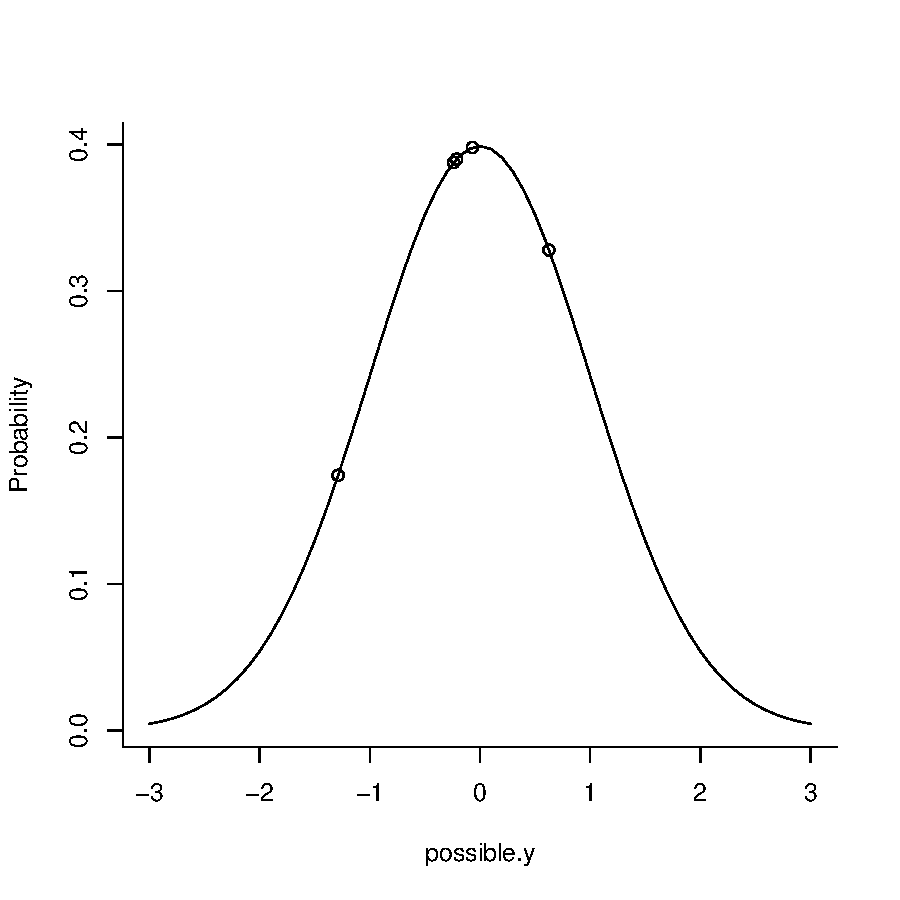
\includegraphics{Lecture1-006}
\end{center}
\caption{Probability density function for the unit normal with the data points overlaid.}
\label{dnorm-fig}
\end{figure}

The likelihood of these data, conditioning on $\mu=0$ and $\sigma^2=1$, is proportional to the product of the densities (read off the y axis on Figure \ref{dnorm-fig}):  

\begin{Schunk}
\begin{Sinput}
> prod(dnorm(Ndata$y, mean = 0, sd = sqrt(1)))
\end{Sinput}
\begin{Soutput}
[1] 0.003015919
\end{Soutput}
\end{Schunk}

Of course we don't know the true mean and variance and so we may want to ask how probable the data would be if, say, $\mu=0$, and $\sigma^2=0.5$:

\iftalk
\else
\fi

\begin{Schunk}
\begin{Sinput}
> prod(dnorm(Ndata$y, mean = 0, sd = sqrt(0.5)))
\end{Sinput}
\begin{Soutput}
[1] 0.005091715
\end{Soutput}
\end{Schunk}

It would seem that the data are more likely under this set of parameters than the true parameters, which we must expect some of the time just from random sampling. To get some idea as to why this might be the case we can overlay the two densities (Figure \ref{dnorm1-fig}), and we can see that although some data points (e.g. 1.2) are more likely with the true parameters, in aggregate the new parameters produce a higher likelihood.\\


\begin{figure}[!h]
\begin{center}
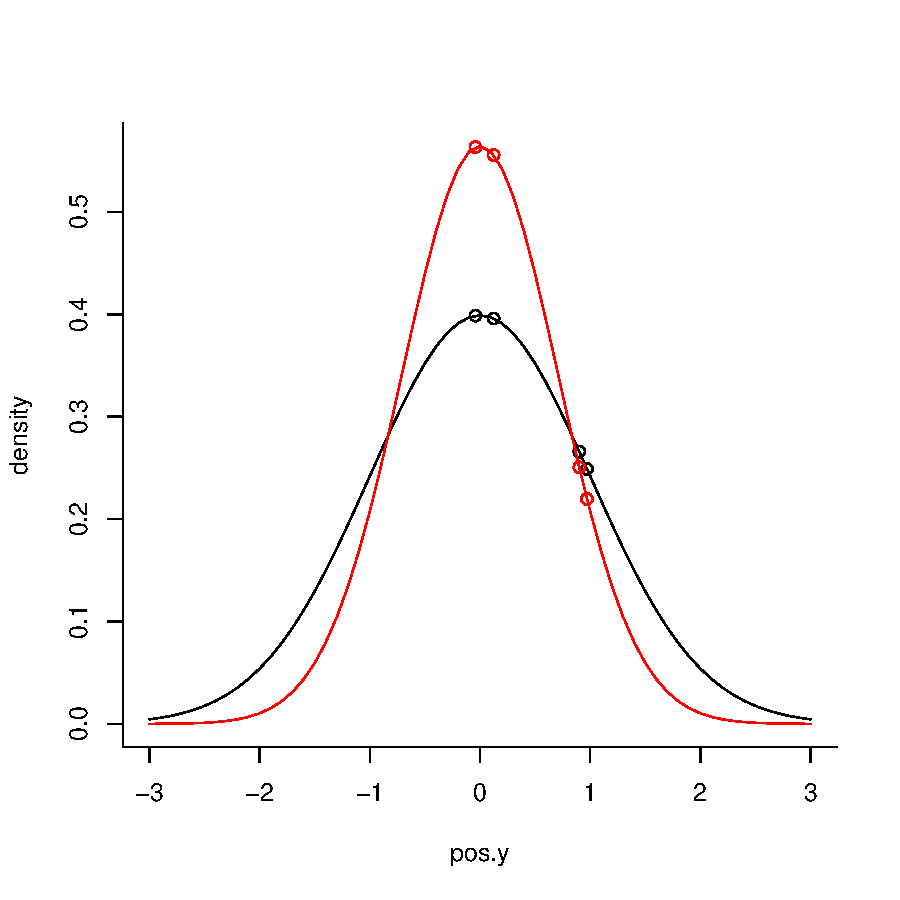
\includegraphics{Lecture1-011}
\end{center}
\caption{Two probability density functions for normal distributions with means of zero, and a variance of one (black line) and a variance of 0.5 (red line).  The data points are overlaid.}
\label{dnorm1-fig}
\end{figure}

The likelihood of the data can be calculated on a grid of possible parameter values to produce a likelihood surface, as in Figure \ref{Lsurface-fig}. The densities on the contours have been scaled so they are relative to the density of the parameter values that have the highest density (the maximum likelihood estimate of the two parameters). Two things are apparent. First, although the surface is symmetric about the line $\mu = \hat{\mu}$ (where $\hat{}$ stands for maximum likelihood estimate) the surface is far from symmetric about the line $\sigma^{2} = \hat{\sigma}^{2}$. Second, there are a large range of parameter values for which the data are only 10 times less likely than if the data were generated under the maximum likelihood estimates.    



\iftalk
\else
\fi

\begin{figure}[!h]
\begin{center}
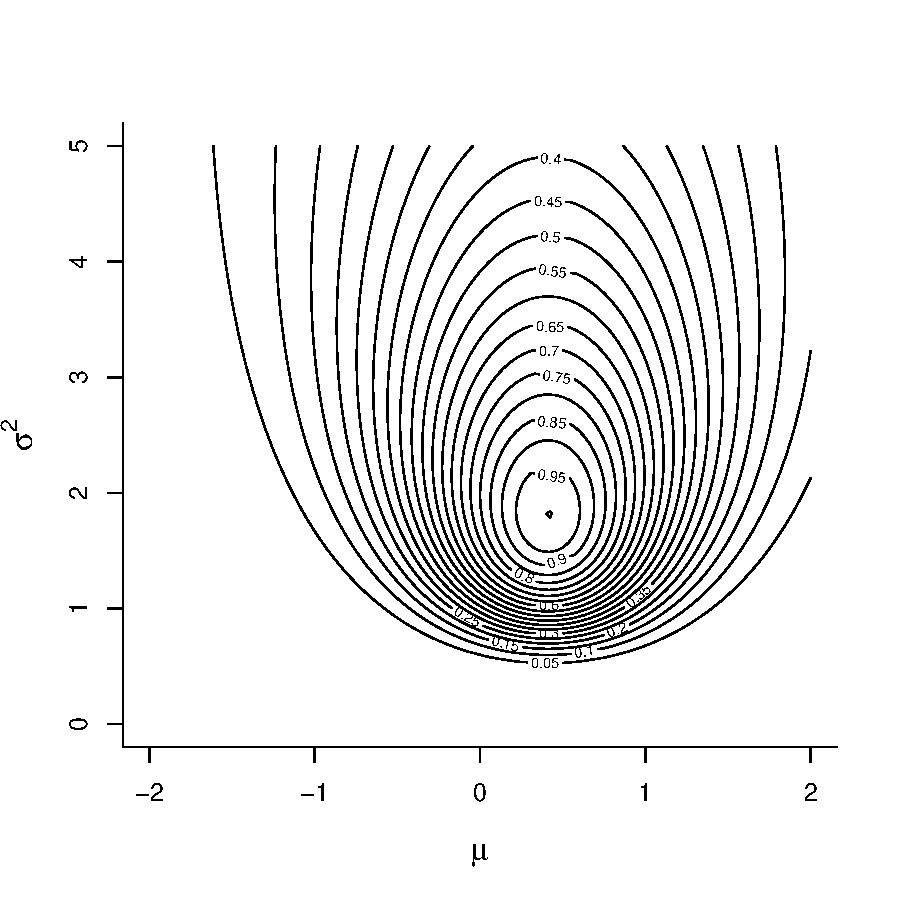
\includegraphics{Lecture1-015}
\end{center}
\caption{Likelihood surface for the likelihood $Pr({\bf y}|\mu, \sigma^{2})$. The likelihood has been normalised so that the maximum likelihood has a value of one.}
\label{Lsurface-fig}
\end{figure}

\subsection{Maximum Likelihood (ML)}

The ML estimator is the combination of $\mu$ and $\sigma^{2}$ that make the data most likely. Although we could evaluate the density on a grid of parameter values (as we did to produce Figure \ref{Lsurface-fig}) in order to locate the maximum, for such a simple problem the ML estimator can be derived analytically. However, so we don't have to meet some nasty maths later, I'll introduce and use one of R's generic optimising routines that can be used to maximise the likelihood function (in practice, the log-likelihood is maximised to avoid numerical problems):


\begin{Schunk}
\begin{Sinput}
> loglik <- function(par, y) {
+     sum(dnorm(y, par[1], sqrt(par[2]), log = TRUE))
+ }
> MLest <- optim(c(mean = 0, var = 1), fn = loglik, 
+     y = Ndata$y, control = list(fnscale = -1, 
+         reltol = 1e-16))$par
\end{Sinput}
\end{Schunk}

\iftalk
\else
\fi

The first call to \texttt{optim} are starting values for the optimisation algorithm, and the second argument (\texttt{fn}) is the function to be maximised. By default \texttt{optim} will try to minimise the function hence multiplying by -1 (\texttt{fnscale = -1}).  The algorithm has successfully found the mode:

\begin{Schunk}
\begin{Sinput}
> MLest
\end{Sinput}
\begin{Soutput}
      mean        var 
-0.1051258  0.4726117 
\end{Soutput}
\end{Schunk}

Alternatively we could also fit the model using \texttt{glm}:

\begin{Schunk}
\begin{Sinput}
> m1a.1 <- glm(y ~ 1, data = Ndata)
> summary(m1a.1)
\end{Sinput}
\begin{Soutput}
Call:
glm(formula = y ~ 1, data = Ndata)

Deviance Residuals: 
       1         2         3         4         5  
-0.03376   1.30494  -0.64260  -0.47012  -0.15846  

Coefficients:
            Estimate Std. Error t value Pr(>|t|)
(Intercept)  -0.1051     0.3437  -0.306    0.775

(Dispersion parameter for gaussian family taken to be 0.5907647)

    Null deviance: 2.3631  on 4  degrees of freedom
Residual deviance: 2.3631  on 4  degrees of freedom
AIC: 14.442

Number of Fisher Scoring iterations: 2
\end{Soutput}
\end{Schunk}
 
Here we see that although the estimate of the mean (intercept) is the same, the estimate of the variance (the dispersion parameter: 0.591) is higher when fitting the model using \texttt{glm}. In fact the ML estimate is a factor of $\frac{n}{n-1}$ smaller.

\begin{Schunk}
\begin{Sinput}
> MLest["var"] * (5/4)
\end{Sinput}
\begin{Soutput}
      var 
0.5907647 
\end{Soutput}
\end{Schunk}

\subsection{Restricted Maximum Likelihood (REML)}

To see why this happens, imagine if we had only observed the first two values of $y$ (Figure \ref{muvar-fig}). The variance is defined as the average squared distance between a random variable and the \emph{true} mean. However, the ML estimator of the variance is the average squared distance between a random variable and the ML \emph{estimate} of the mean. Since the ML estimator of the mean is the average of the two numbers (the dashed line) then the average squared distance will always be smaller than if the true mean was used, unless the ML estimate of the mean and the true mean coincide. This is why we divide by $n-1$ when estimating the variance from the sum of squares, and is the motivation behind REML.

\iftalk
\else
\fi

\begin{figure}[!h]
\begin{center}
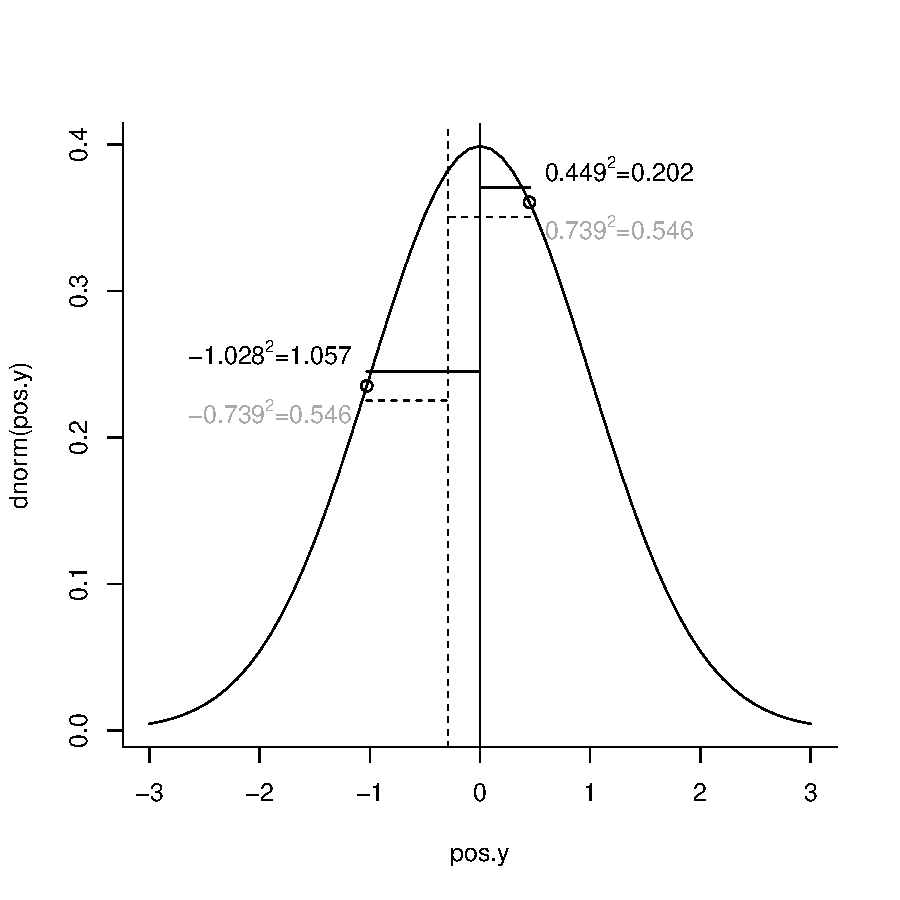
\includegraphics{Lecture1-023}
\end{center}
\caption{Probability density function for the unit normal with 2 realisations overlaid. The solid vertical line is the true mean, whereas the vertical dashed line is the mean of the two realisations (the ML estimator of the mean). The variance is the expected squared distance between the true mean and the realisations. The ML estimator of the variance is the average squared distance between the ML mean and the realisations (horizontal dashed lines), which is always smaller than the average squared distance between the true mean and the realisations (horizontal solid lines)}
\label{muvar-fig}
\end{figure}

\newpage
\section{Prior Distribution}

\texttt{MCMCglmm} uses an inverse Wishart prior for the (co)variances and a normal prior for the fixed effects. In versions $>1.13$ parameter expanded models can be used which enable prior specifications from the the scaled non-central F-distribution \citep{Gelman.2006}. Here, we will focus on specifying a prior for a single fixed effect ($\mu$) and a single variance component using the inverse-Wishart to highlight some of the issues. I strongly recommend reading the section \ref{secPX-p} on parameter expanded priors as these can be less informative than the inverse-Wishart under many situations.\\

For a single variance component the inverse Wishart takes two scalar parameters, \texttt{V} and \texttt{nu}. The distribution tends to a point mass on \texttt{V} as the degree of belief parameter, \texttt{nu} goes to infinity. The distribution tends to be right skewed when \texttt{nu} is not very large, with a mode of $\frac{\texttt{V}^{\ast}\texttt{nu}}{\texttt{nu}+2}$ but a mean of $\frac{\texttt{V}^{\ast}\texttt{nu}}{\texttt{nu}-2}$ (which is not defined for $\texttt{nu}<2$).\footnote{The inverse gamma is a special case of the inverse Wishart, although it is parametrised using \texttt{shape} and \texttt{scale}, where $\texttt{nu}=2\ast\texttt{shape}$ and $\texttt{V} = \frac{\texttt{scale}}{\texttt{shape}}$ (or $\texttt{shape} = \frac{\texttt{nu}}{2}$ and $\texttt{scale} = \frac{\texttt{nu}*\texttt{V}}{2}$). \texttt{MCMCpack} provides a density function (\texttt{dinvgamma}) for the inverse gamma distribution.}\\

As before, we can evaluate and plot density functions in order to visualise what the distribution looks like. Figure \ref{dinvgamma-fig} plots the probability density functions holding \texttt{V} equal to one but with \texttt{nu} varying.\\

\iftalk
\else
\fi

\iftalk
\else
\fi

\begin{figure}[!h]
\begin{center}
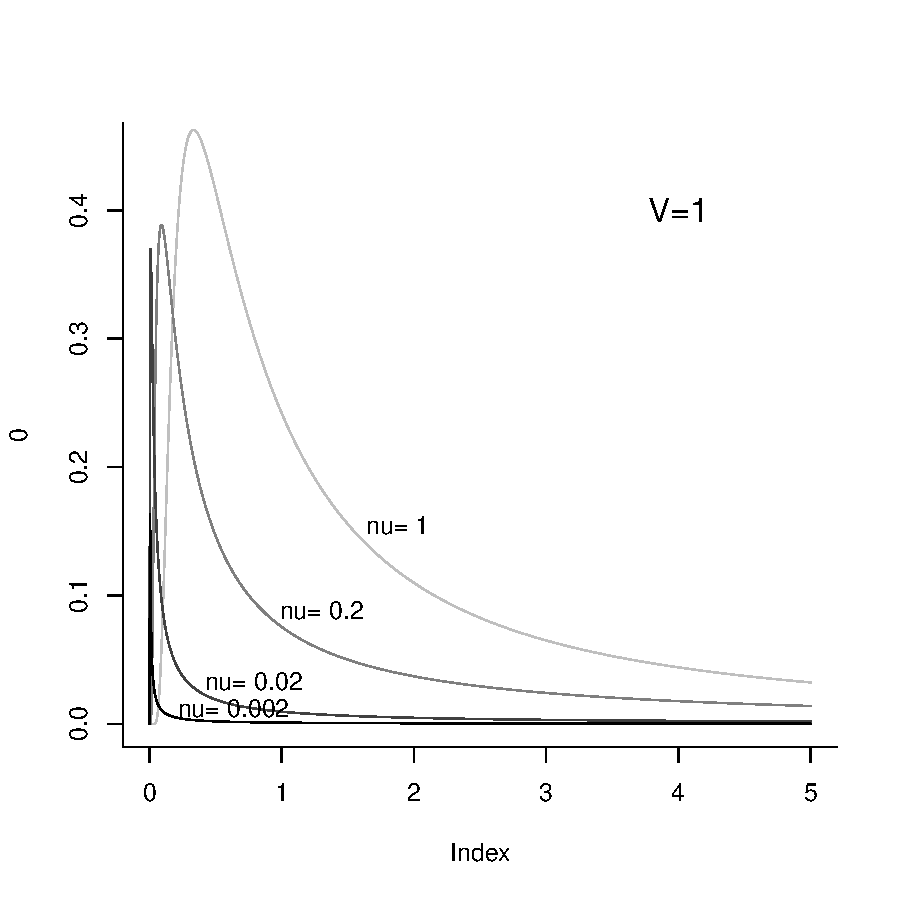
\includegraphics{Lecture1-027}
\end{center}
\caption{Probability density function for a univariate inverse Wishart with the variance at the limit set to 1 (\texttt{V=1}) and varying degree of belief parameter (\texttt{nu}). With \texttt{V=1} these distributions are equivalent to inverse gamma distributions with shape and scale parameters set to \texttt{nu}/2.}
\label{dinvgamma-fig}
\end{figure}

A probability distribution must integrate to one because a variable must have some value. It therefore seems reasonable that when specifying a prior, care must be taken that this condition is met. In the example here where \texttt{V} is a single variance this condition is met if \texttt{V>0} and \texttt{nu>0}.  If this condition is not met then the prior is said to be improper, and in WinBUGS (and possibly other software) improper priors cannot be specified.  Although great care has to be taken when using improper priors, \texttt{MCMCglmm} does allow them as they have some useful properties, and some common improper priors are discussed in section \ref{IP-sec}. However, for now we will use the prior specification \texttt{V=1} and \texttt{nu=0.002} which is frequently used for variance components. For the mean we will use a diffuse normal prior centred around zero but with very large variance ($10^{8}$). If the variance is finite then the prior is always proper.\\

As before we can write a function for calculating the (log) prior probability:

\begin{Schunk}
\begin{Sinput}
> logprior <- function(par, priorR, priorB) {
+     dnorm(par[1], mean = priorB$mu, sd = sqrt(priorB$V), 
+         log = TRUE) + log(dinvgamma(par[2], shape = priorR$nu/2, 
+         scale = (priorR$nu * priorR$V)/2))
+ }
\end{Sinput}
\end{Schunk}

where \texttt{priorR} is a list with elements \texttt{V} and \texttt{nu} specifying the prior for the variance, and \texttt{priorB} is a list with elements \texttt{mu} and \texttt{V} specifying the prior for the mean. \texttt{MCMCglmm} takes these prior specifications as a list: 

\begin{Schunk}
\begin{Sinput}
> prior <- list(R = list(V = 1, nu = 0.002), B = list(mu = 0, 
+     V = 1e+08))
\end{Sinput}
\end{Schunk}


\section{Posterior Distribution}

  To obtain a posterior density we need to multiply the likelihood by the prior probability for that set of parameters. We can write a function for doing this: 

\begin{Schunk}
\begin{Sinput}
> loglikprior <- function(par, y, priorR, priorB) {
+     loglik(par, y) + logprior(par, priorR, priorB)
+ }
\end{Sinput}
\end{Schunk}

and we can overlay the posterior densities on the likelihood surface we calculated before (Figure \ref{Lsurface-fig}).\\


\iftalk
\else
\fi

\begin{figure}[!h]
\begin{center}
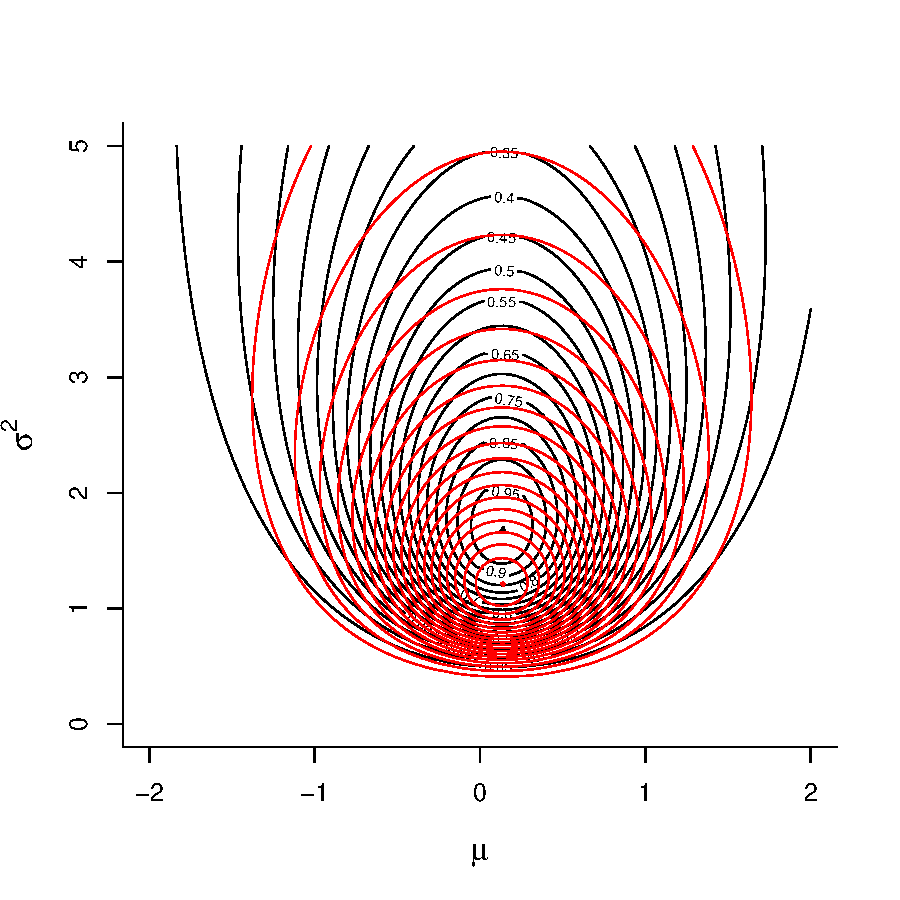
\includegraphics{Lecture1-034}
\end{center}
\caption{Likelihood surface for the likelihood $Pr({\bf y}|\mu, \sigma^{2})$ in black, and the posterior distribution $Pr(\mu, \sigma^{2} | {\bf y})$ in red.  The likelihood has been normalised so that the maximum likelihood has a value of one, and the posterior distribution has been normalised so that the posterior mode has a value of one. The prior distributions  $Pr(\mu)\sim N(0, 10^8)$ and  $Pr(\sigma^{2})\sim IW(\texttt{V}=1, \texttt{nu}=0.002)$ were used.}
\label{Psurface-fig}
\end{figure}


The prior has some influence on the posterior mode of the variance, and we can use an optimisation algorithm again to locate the mode:  

\begin{Schunk}
\begin{Sinput}
> Best <- optim(c(mean = 0, var = 1), fn = loglikprior, 
+     y = Ndata$y, priorR = prior$R, priorB = prior$B, 
+     method = "L-BFGS-B", lower = c(-1e+05, 1e-05), 
+     upper = c(1e+05, 1e+05), control = list(fnscale = -1, 
+         factr = 1e-16))$par
> Best
\end{Sinput}
\begin{Soutput}
      mean        var 
-0.1051258  0.3377710 
\end{Soutput}
\end{Schunk}

\iftalk
\else
\fi

The posterior mode for the mean is identical to the ML estimate, but the posterior mode for the variance is even less than the ML estimate which is known to be downwardly biased. The reason that the ML estimate is downwardly biased is because it did no take into account the uncertainty in the mean. In a Bayesian analysis we can do this by evaluating the marginal distribution of $\sigma^{2}$ and averaging over the uncertainty in the mean.

\subsection{Marginal Posterior Distribution}

The marginal distribution is often of primary interest in statistical inference, because it represents our knowledge about a parameter given the data: 

\begin{displaymath}
Pr(\sigma^{2} | {\bf y}) \propto \int Pr(\mu, \sigma^{2} | {\bf y})d\mu
\label{marg-eq}
\end{displaymath}

after averaging over any nuisance parameters, such as the mean in this case.\\  

Obtaining the marginal distribution analytically is usually impossible, and this is where MCMC approaches prove useful.  We can fit this model in \texttt{MCMCglmm} pretty much in the same way as we did using \texttt{glm}:


\begin{Schunk}
\begin{Sinput}
> m1a.2 <- MCMCglmm(y ~ 1, data = Ndata, prior = prior, 
+     thin = 1, verbose = FALSE)
\end{Sinput}
\end{Schunk}

The Markov chain is drawing random (but often correlated) samples from the joint posterior distribution (depicted by the red contours in Figure \ref{Psurface-fig}).  The element of the output called \texttt{Sol} contains the distribution for the mean, and the element called \texttt{VCV} contains the distribution for the variance. We can produce a scatter plot:

\begin{Schunk}
\begin{Sinput}
> points(cbind(m1a.2$Sol, m1a.2$VCV))
\end{Sinput}
\end{Schunk}

and we see that MCMCglmm is sampling the same distribution as the posterior distribution calculated on a grid of possible parameter values (Figure \ref{PsurfaceMCMC-fig}).\\

\iftalk
\else
\fi

\begin{figure}[!h]
\begin{center}
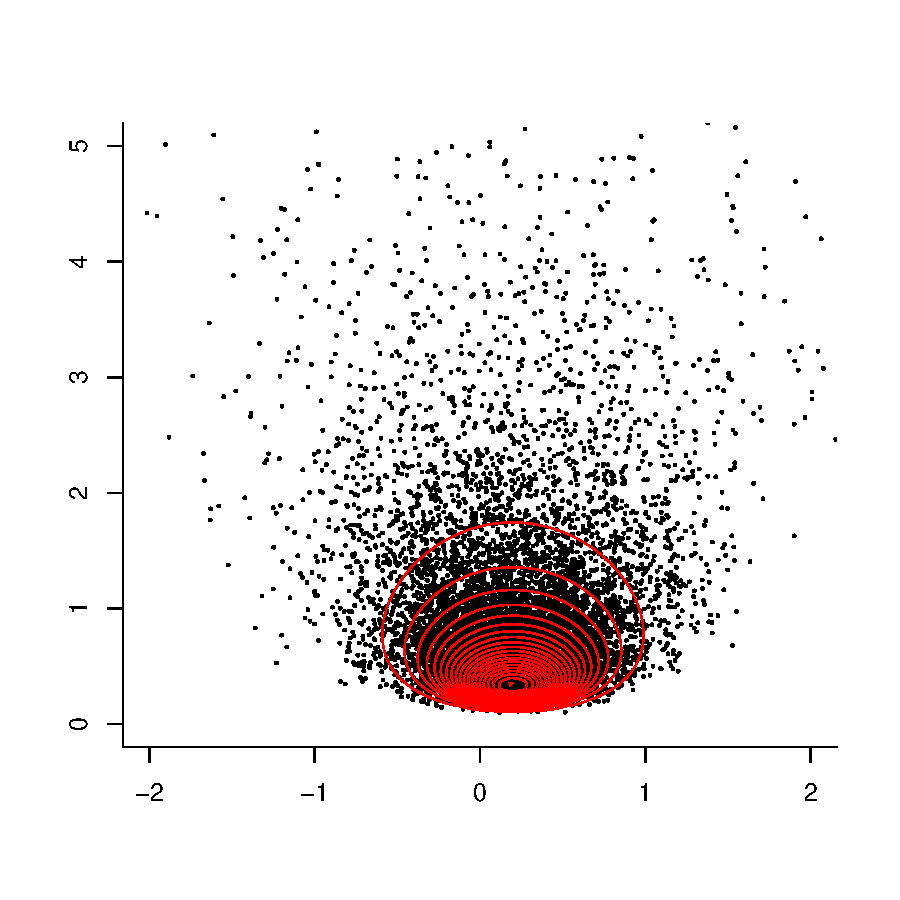
\includegraphics{Lecture1-041}
\end{center}
\caption{The posterior distribution $Pr(\mu, \sigma^{2} | {\bf y})$. The black dots are samples from the posterior using MCMC, and the red contours are calculated by evaluating the posterior density on a grid of parameter values. The contours are normalised so that the posterior mode has a value of one.}
\label{PsurfaceMCMC-fig}
\end{figure}

A very nice property of MCMC is that we can normalise the density so that it integrates to 1 (a true probability) rather than normalising it with respect to some other aspect of the distribution, such as the density at the ML estimator or the joint posterior mode as in Figures \ref{Lsurface-fig} and \ref{Psurface-fig}. To make this clearer, imagine we wanted to know how much more probable the unit normal (i.e. with $\mu=0$ and $\sigma^{2}=1$) was than a normal distribution with the posterior modal parameters. We can calculate this by taking the ratio of the posterior densities at these two points:  \\ 
 

\begin{Schunk}
\begin{Sinput}
> exp(loglikprior(Best, Ndata$y, prior$R, prior$B) - 
+     loglikprior(c(0, 1), Ndata$y, prior$R, prior$B))
\end{Sinput}
\begin{Soutput}
[1] 4.522744
\end{Soutput}
\end{Schunk}


Now, if we wanted to know the probability that the parameters lay in the region of parameter space we were plotting, i.e. lay in the square $\mu = (-2,2)$ and $\sigma^{2} = (0,5)$ then this would be more difficult. We would have to evaluate the density at a much larger range of parameter values than we had done, ensuring that we had covered all regions with positive probability. Because MCMC has sampled the distribution randomly, this probability will be equal to the expected probability that we have drawn an MCMC sample from the region. We can obtain an estimate of this by seeing what proportion of our actual samples lie in this square:

\begin{Schunk}
\begin{Sinput}
> prop.table(table(m1a.2$Sol > -2 & m1a.2$Sol < 
+     2 & m1a.2$VCV < 5))
\end{Sinput}
\begin{Soutput}
 FALSE   TRUE 
0.0225 0.9775 
\end{Soutput}
\end{Schunk}

There is Monte Carlo error in the answer (0.978) but if we collect a large number of samples then this can be minimised.\\ 

Using a similar logic we can obtain the marginal distribution of the variance by simply evaluating the draws in \texttt{VCV} ignoring (averaging over) the draws in \texttt{Sol}:

\iftalk
\else
\begin{Schunk}
\begin{Sinput}
> hist(m1a.2$VCV[which(m1a.2$VCV < 5)])
> abline(v = Best["var"], col = "red")
\end{Sinput}
\end{Schunk}
\fi

\begin{figure}[!h]
\begin{center}
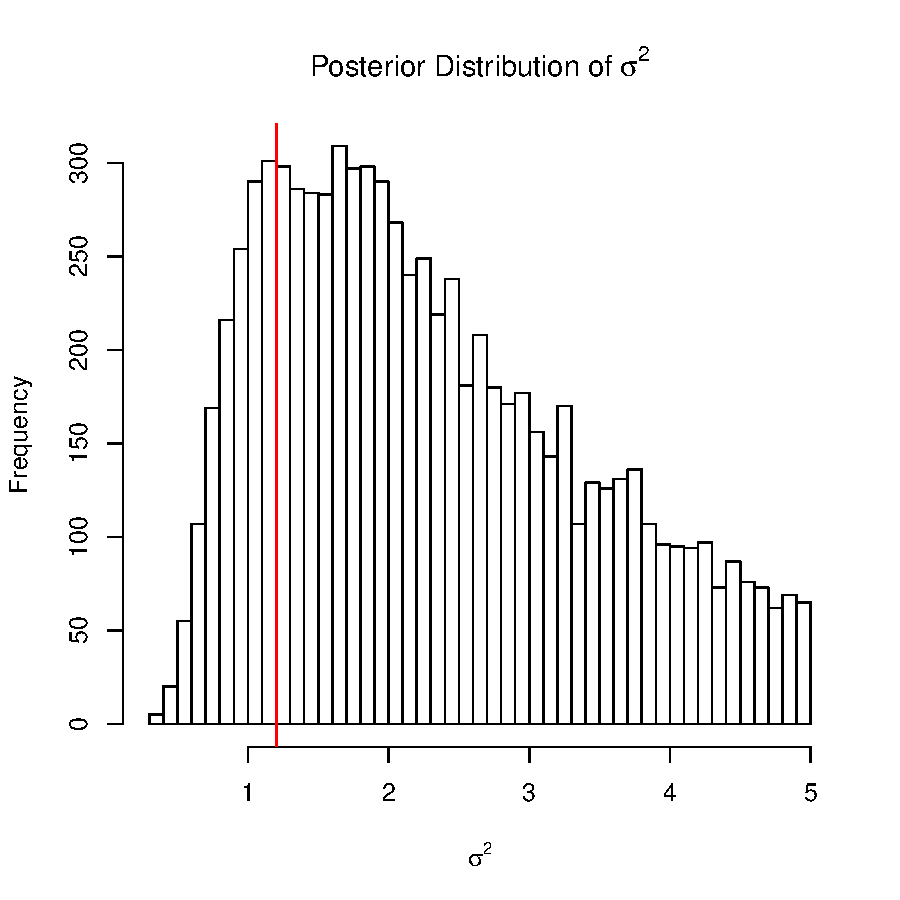
\includegraphics{Lecture1-049}
\end{center}
\caption{Histogram of samples from the marginal distribution of the variance $Pr(\sigma^{2} | {\bf y})$ using MCMC. The vertical line is the joint posterior mode, which differs slightly from the marginal posterior mode (the peak of the marginal distribution).}
\label{PsurfaceMCMC-fig}
\end{figure}

In this example (see Figure \ref{PsurfaceMCMC-fig}) the marginal mode and the joint mode are very similar, although this is not necessarily the case and can depend both on the data and the prior. Section \ref{IP-sec} introduces improper priors that are non-informative with regard to the marginal distribution of a variance.\\

\section{MCMC}

In order to be confident that \texttt{MCMCglmm} has successfully sampled the posterior distribution it will be necessary to have a basic understanding of MCMC methods. MCMC methods are often used when the joint posterior distribution cannot be derived analytically, which is nearly always the case. MCMC relies on the fact that although we cannot derive the complete posterior, we can calculate the height of the posterior distribution at a particular set of parameter values, as we did to obtain the contour plot in Figure \ref{Psurface-fig}. However, rather than going systematically through every likely combination of $\mu$ and $\sigma$ and calculate the height of the distribution at regular distances, MCMC moves stochastically through parameter space, hence the name `Monte Carlo'.\\   

\subsection{Starting values}

First we need to initialise the chain and specify a set of parameter values from which the chain can start moving through parameter space. Ideally we would like to pick a region of high probability, as we do not want to waste time wandering through regions of low probability: we are not so interested in determining the height of the distribution far outside of  Figure \ref{Psurface-fig} as it is virtually flat and close to zero (or at least we hope so!).  Although starting configurations can be set by the user using the \texttt{start} argument, in general the heuristic techniques used by \texttt{MCMCglmm} seem to work quite well. We will denote the parameter values of the starting configuration (time $t=0$) as $\mu_{t=0}$ and ${\sigma^{2}}_{t=0}$. There are several ways in which we can get the chain to move in parameter space, and \texttt{MCMCglmm} uses a combination of Gibbs sampling, slice sampling and Metropolis-Hastings updates. To illustrate, it will be easier to turn the contour plot of the posterior distribution into a perspective plot (Figure \ref{Psurface.persp-fig}).

  

\begin{figure}[!h]
\begin{center}
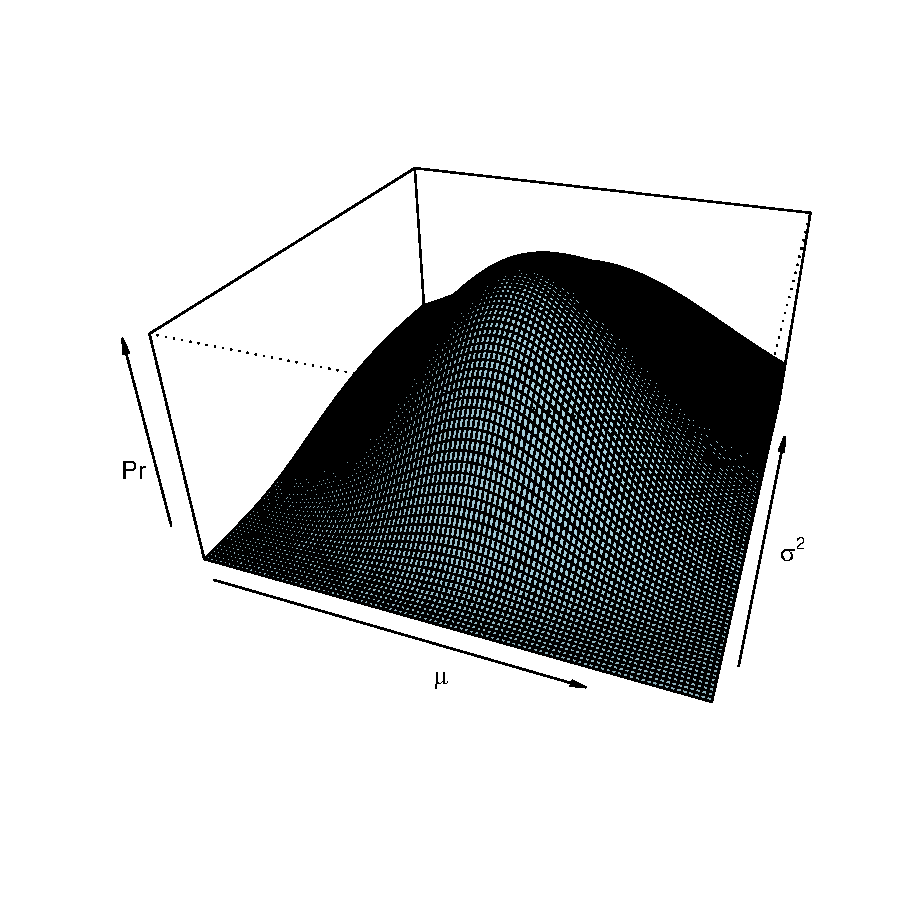
\includegraphics{Lecture1-052}
\end{center}
\caption{The posterior distribution $Pr(\mu, \sigma^{2} | {\bf y})$. This perspective plot is equivalent to the contour plot in Figure \ref{Psurface-fig}}
\label{Psurface.persp-fig}
\end{figure}


\subsection{Metrpolis-Hastings updates}

After initialising the chain we need to decide where to go next, and this decision is based on two rules.  First we have to generate a candidate destination, and then we need to decide whether to go there or stay where we are.  There are many ways in which we could generate candidate parameter values, and \texttt{MCMCglmm} uses a well tested and simple method. A random set of coordinates are picked from a multivariate normal distribution that is entered on the initial coordinates  $\mu_{t=0}$ and $\sigma^{2}_{t=0}$.  We will denote this new set of parameter values as  $\mu_{new}$ and $\sigma^{2}_{new}$. The question then remains whether to move to this new set of parameter values or remain at our current parameter values now designated as old $\mu_{old}=\mu_{t=0}$ and $\sigma^{2}_{old}=\sigma^{2}_{t=0}$.  If the posterior probability for the new set of parameter values is greater, then the chain moves to this new set of parameters and the chain has successfully completed an iteration: ($\mu_{t=1} = \mu_{new}$ and $\sigma^{2}_{t=1}=\sigma^{2}_{new}$).  If the new set of parameter values has a lower posterior probability then the chain may move there, but not all the time.  The probability that the chain moves to low lying areas, is determined by the relative difference between the old and new posterior probabilities.  If the posterior probability for $\mu_{new}$ and $\sigma^{2}_{new}$ is 5 times less than the posterior probability for $\mu_{old}$ and $\sigma^{2}_{old}$, then the chain would move to the new set of parameter values 1 in 5 times. If the move is successful then we set $\mu_{t=1} = \mu_{new}$ and $\sigma^{2}_{t=1}=\sigma^{2}_{new}$ as before, and if the move is unsuccessful then the chain stays where it is ($\mu_{t=1} = \mu_{old}$ and $\sigma^{2}_{t=1}=\sigma^{2}_{old}$).  Using these rules we can record where the chain has travelled and generate an approximation of the posterior distribution.  Basically, a histogram of Figure \ref{Psurface.persp-fig}.\\
 
\subsection{Gibbs Sampling}

Gibbs sampling is a special case of Metropolis-Hastings updating, and \texttt{MCMCglmm} uses Gibbs sampling to update most parameters.  In the Metropolis-Hastings example above, the Markov Chain was allowed to move in both directions of parameter space simultaneously.  An equally valid approach would have been to set up two Metropolis-Hastings schemes where the chain was first allowed to move along the $\mu$ axis, and then along the $\sigma^{2}$ axis. In Figure \ref{Psurface.persp2-fig} I have cut the posterior distribution of Figure \ref{Psurface.persp-fig} in half, and the edge of the surface facing left is the conditional distribution of $\mu$ given that $\sigma^{2}=1$:


\begin{equation}
Pr(\mu |\sigma^{2}=1, \bm{y}).
\end{equation}




\begin{figure}[!h]
\begin{center}
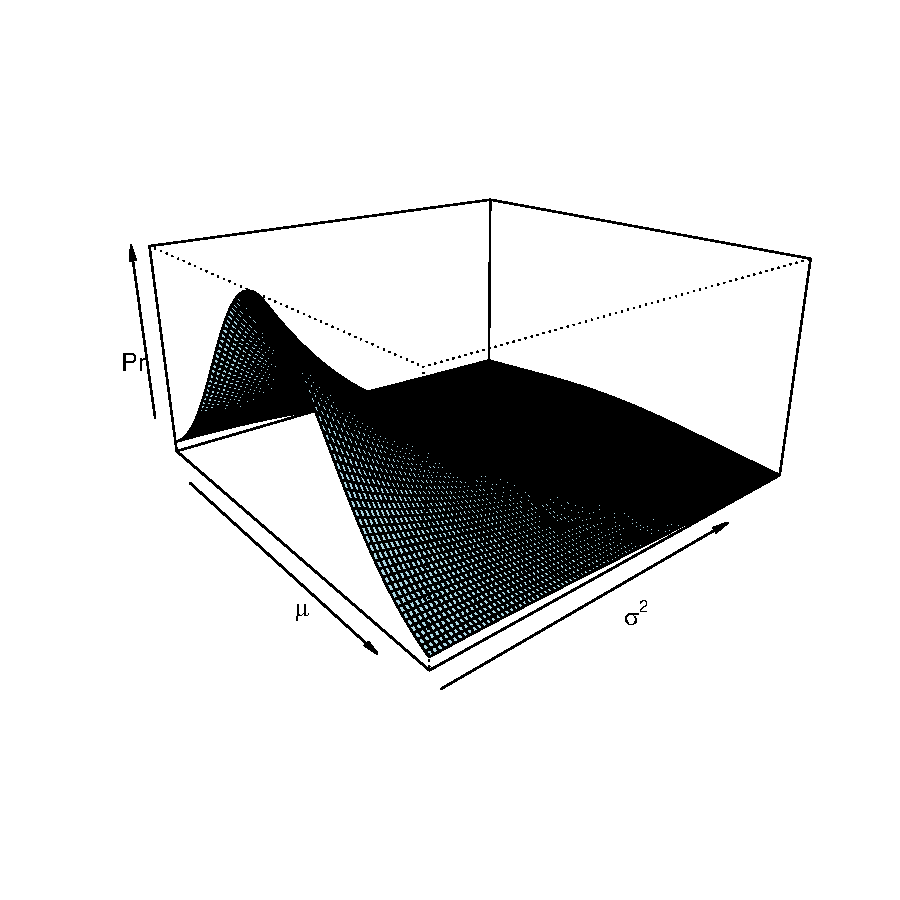
\includegraphics{Lecture1-055}
\end{center}
\caption{The posterior distribution $Pr(\mu, \sigma^{2} | {\bf y})$, but only for values of $\sigma^{2}$ between 1 and 5, rather than 0 to 5 (Figure \ref{Psurface.persp-fig}). The 
edge of the surface facing left is the conditional distribution of the mean when $\sigma^{2}=1$ ($Pr(\mu | {\bf y}, \sigma^{2}=1)$). This conditional distribution follows a normal distribution.}
\label{Psurface.persp2-fig}
\end{figure}

 In some cases, the equation that describes this conditional distribution can be derived despite the equation for the complete joint distribution of Figure \ref{Psurface.persp-fig} remaining unknown.  When the conditional distribution of $\mu$ is known we can use Gibbs sampling. Lets say the chain at a particular iteration is located at $\sigma^{2}=1$.  If we updated $\mu$ using a Metropolis-Hastings algorithm we would generate a candidate value and evaluate its relative probability compared to the old value.  This procedure would take place in the slice of posterior facing left in Figure \ref{Psurface.persp2-fig}. However, because we know the actual equation for this slice we can just generate a new value of $\mu$ directly. This is Gibbs sampling.  The slice of the posterior that we can see in Figure \ref{Psurface.persp2-fig} actually has a normal distribution. Because of the weak prior this normal distribution has a mean close to the mean of $\bf{y}$ and a variance close to $\frac{\sigma^{2}}{n} = \frac{1}{n}$.  Gibbs sampling can be much more efficient than Metropolis-Hastings updates, especially when high dimensional conditional distributions are known, as is typical in GLMMs. A technical description of the sampling schemes used by \texttt{MCMCglmm} is given in appendix \ref{MCMC-app}, but is perhaps not important to know.

\subsection{Slice Sampling}

If the distribution can be factored such that one factor is a distribution from which truncated random variables can be drawn, then the slice sampling methods of \citet{Damien.1999} can be used. The latent variables in univariate binary models can be updated in this way if \texttt{slice=TRUE} is specified in the call to \texttt{MCMCglmm}. In these models, slice sampling is only marginally more efficient than adaptive Metropolis-Hastings updates when the residual variance is fixed. However, for parameter expanded binary models where the residual variance is not fixed, the slice sampler can be much more efficient.

\subsection{MCMC Diagnostics}

When fitting a model using \texttt{MCMCglmm} the parameter values through which the Markov chain has travelled are stored and returned.  The length of the chain (the number of iterations) can be specified using the \texttt{nitt} argument\footnote{The double \texttt{t} is because I cannot spell.} (the default is 13,000), and should be long enough so that the posterior approximation is valid.  If we had known the joint posterior distribution in Figure \ref{Psurface.persp-fig} we could have set up a Markov chain that sampled directly from the posterior.  If this had been the case, each successive value in the Markov chain would be independent of the previous value after conditioning on the data, ${\bf y}$, and a thousand iterations of the chain would have produced a histogram that resembled Figure \ref{Psurface.persp-fig} very closely.  However, generally we do not know the joint posterior distribution of the parameters, and for this reason the parameter values of the Markov chain at successive iterations are usually not independent and care needs to be taken regarding the validity of the approximation.  \texttt{MCMCglmm} returns the Markov chain as \texttt{mcmc} objects, which can be analysed using the \texttt{coda} package.  The function \texttt{autocorr} estimates the level of non-independence between successive samples in the chain:

\begin{Schunk}
\begin{Sinput}
> autocorr(m1a.2$Sol)
\end{Sinput}
\begin{Soutput}
, , (Intercept)

         (Intercept)
Lag 0   1.0000000000
Lag 1  -0.0157652146
Lag 5   0.0094886774
Lag 10  0.0093923394
Lag 50  0.0002389178
\end{Soutput}
\begin{Sinput}
> autocorr(m1a.2$VCV)
\end{Sinput}
\begin{Soutput}
, , units

              units
Lag 0   1.000000000
Lag 1   0.175580402
Lag 5  -0.007972959
Lag 10 -0.011741307
Lag 50  0.003373268
\end{Soutput}
\end{Schunk}

 The correlation between successive samples is low for the mean (-0.016) but a bit high for the variance (0.176).  When auto-correlation is high the chain needs to be run for longer, and this can lead to storage problems for high dimensional problems. The argument \texttt{thin} can be passed to \texttt{MCMCglmm} specifying the intervals at which the Markov chain is stored. In model \texttt{m1a.2} we specified \texttt{thin=1} meaning we stored every iteration (the default is \texttt{thin=10}). I usually aim to store 1,000-2,000 iterations and have the autocorrelation between successive \emph{stored} iterations less than 0.1.\\

The approximation obtained from the Markov chain is conditional on the set of parameter values that were used to initialise the chain.  In many cases the first iterations show a strong dependence on the starting parametrisation, but as the chain progresses this dependence may be lost.  As the dependence on the starting parametrisation diminishes the chain is said to converge and the argument \texttt{burnin} can be passed to \texttt{MCMCped} specifying the number of iterations which must pass before samples are stored. The default burn-in period is 3,000 iterations. Assessing convergence of the chain is notoriously difficult, but visual inspection and diagnostic tools such as \texttt{gelman.diag} often suffice.

\begin{Schunk}
\begin{Sinput}
> plot(m1a.2$Sol)
\end{Sinput}
\end{Schunk}

\begin{figure}[!h]
\begin{center}
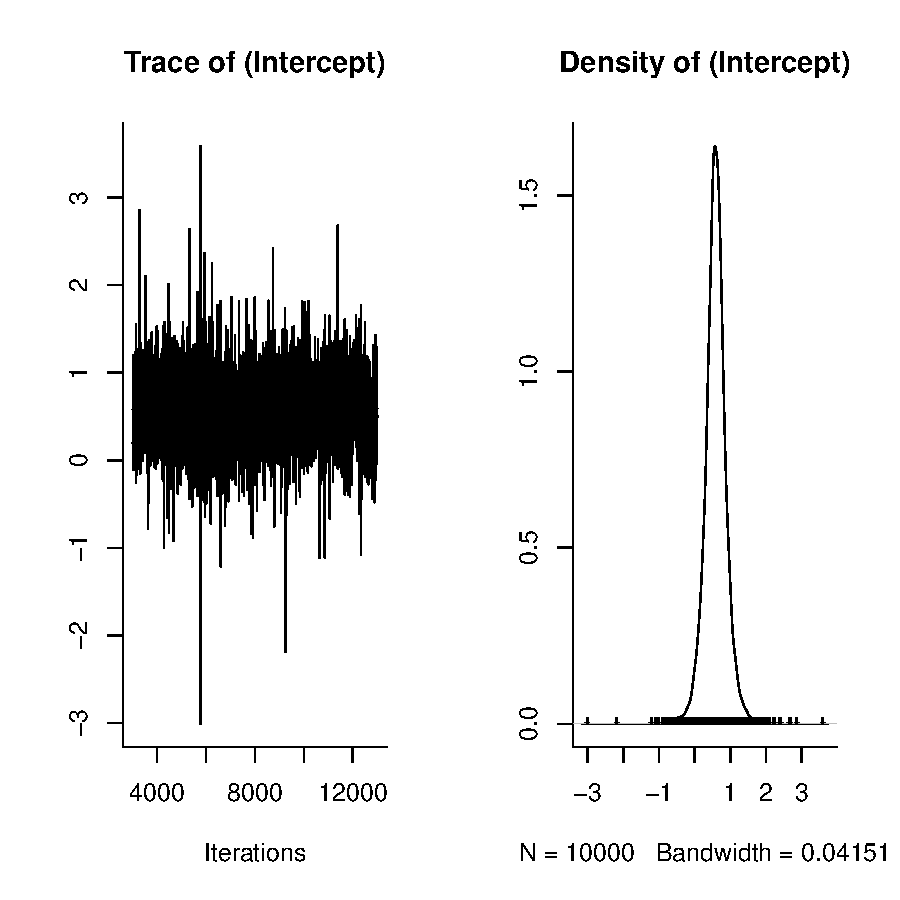
\includegraphics{Lecture1-058}
\end{center}
\caption{Summary plot of the Markov Chain for the intercept.  The left plot is a trace of the sampled posterior, and can be thought of as a time series.  The right plot is a density estimate, and can be thought of a smoothed histogram approximating the posterior.}
\label{time.series-fig}
\end{figure}

On the left of Figure \ref{time.series-fig} is a time series of the parameter as the MCMC iterates, and on the right is a posterior density estimate of the parameter (a smoothed histogram of the output). If the model has converged there should be no trend in the time series. The equivalent plot for the variance is a little hard to see on the original scale, but on the log scale the chain looks good (Figure \ref{time.series2-fig}):


\begin{Schunk}
\begin{Sinput}
> plot(log(m1a.2$VCV))
\end{Sinput}
\end{Schunk}

\begin{figure}[!h]
\begin{center}
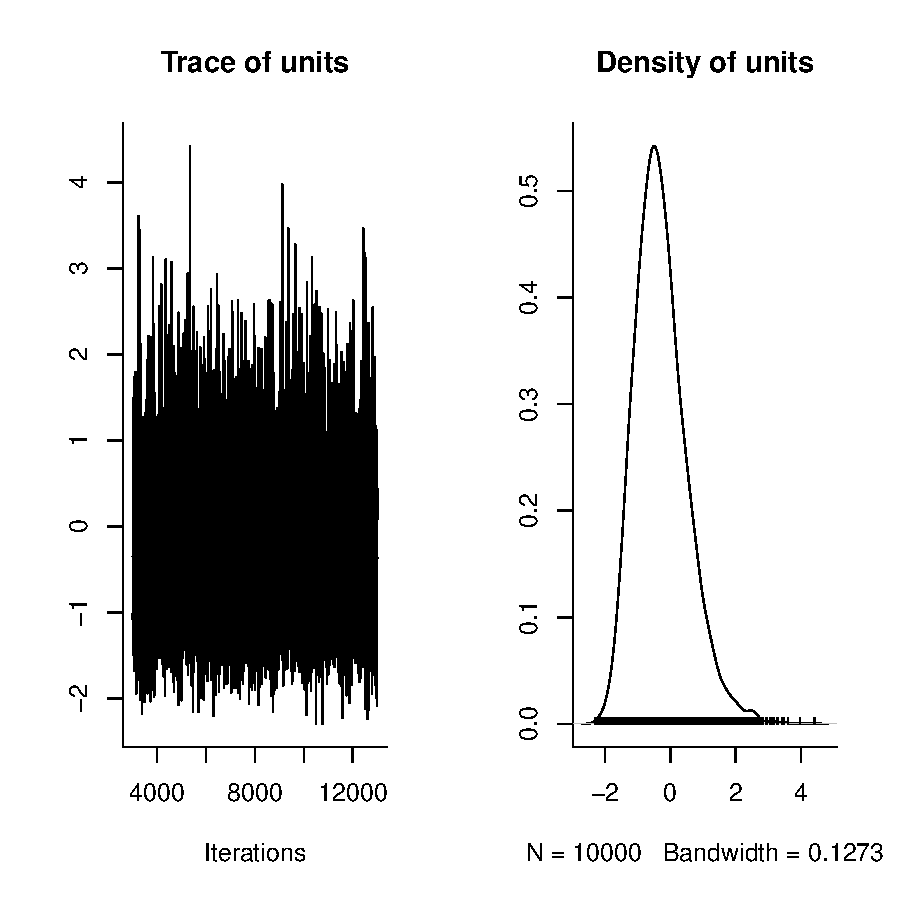
\includegraphics{Lecture1-060}
\end{center}
\caption{Summary plot of the Markov Chain for the logged variance. The logged variance was plotted rather than the variance because it was easier to visualise. The left plot is a trace of the sampled posterior, and can be thought of as a time series.  The right plot is a density estimate, and can be thought of a smoothed histogram approximating the posterior.}
\label{time.series2-fig}
\end{figure}


\section{Improper Priors}
\label{IP-sec}

When improper priors are used their are two potential problems that may be encountered. The first is that if the data do not contain enough information the posterior distribution itself may be improper, and any results obtained from \texttt{MCMCglmm} will be meaningless. In addition, with proper priors there is a zero probability of a variance component being exactly zero but this is not necessarily the case with improper priors.  This can produce numerical problems (trying to divide through by zero) and can also result in a reducible chain. A reducible chain is one which gets `stuck' at some parameter value and cannot escape. This is usually obvious from the \texttt{mcmc} plots but \texttt{MCMCglmm} will often terminate before the analysis has finished with an error message of the form:

\begin{Schunk}
\begin{Soutput}
ill-conditioned G/R structure: use proper priors ...
\end{Soutput}
\end{Schunk}  

However, improper priors do have some useful properties.
 
\subsection{Flat Improper Prior}

The simplest improper prior is one that is proportional to some constant for all possible parameter values. This is known as a flat prior and the posterior density in such cases is equal to the likelihood:

\begin{displaymath}
Pr(\mu, \sigma^{2} | {\bf y}) \propto Pr({\bf y} | \mu, \sigma^{2})
\label{fprior-eq}
\end{displaymath}

It is known that although such a prior is non-informative for the mean it is informative for the variance. We can specify a flat prior on the variance component by having \texttt{nu=0} (the value of \texttt{V} is irrelevant) and the default prior for the mean is so diffuse as to be essentially flat across the range ($-10^6, 10^6$).   

\begin{Schunk}
\begin{Sinput}
> prior.m1a.3 <- list(R = list(V = 1, nu = 0))
> m1a.3 <- MCMCglmm(y ~ 1, data = Ndata, thin = 1, 
+     prior = prior.m1a.3, verbose = FALSE)
\end{Sinput}
\end{Schunk}

We can overlay the joint posterior distribution on the likelihood surface (\ref{Psurface.flat-fig}) and see that the two things are in close agreement, up to Monte Carlo error.
 

\iftalk
\else
\fi

\begin{figure}[!h]
\begin{center}
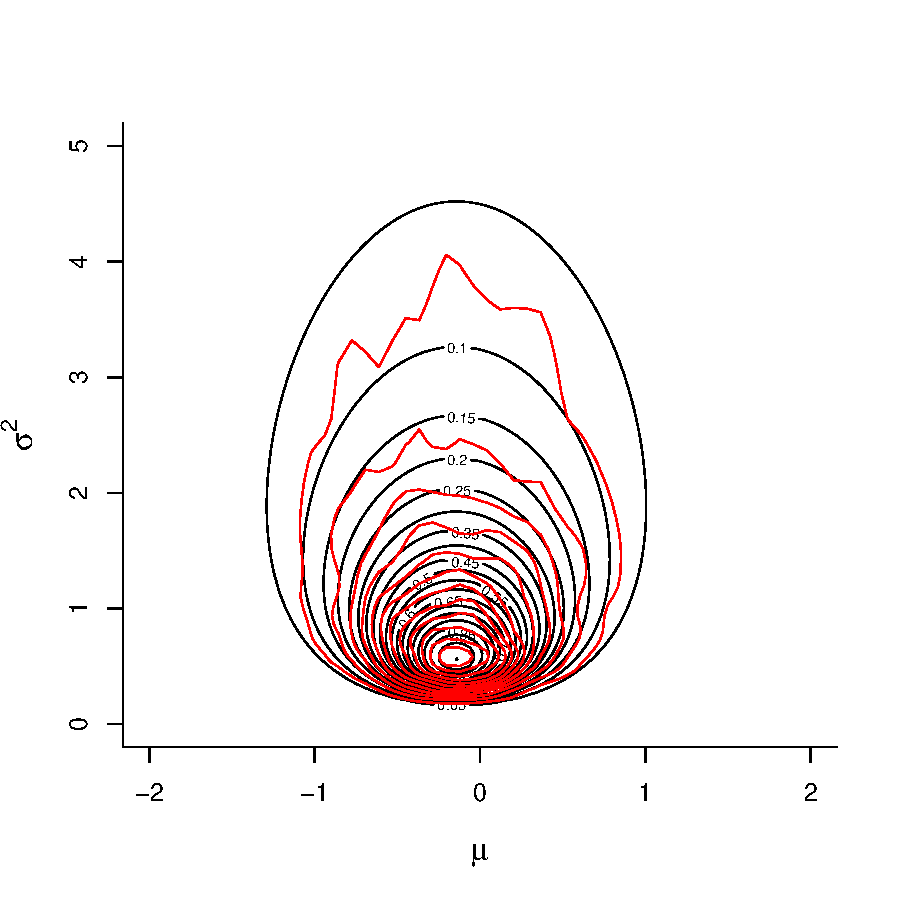
\includegraphics{Lecture1-065}
\end{center}
\caption{Likelihood surface for the likelihood $Pr({\bf y}|\mu, \sigma^{2})$ in black, and an MCMC approximation for the posterior distribution $Pr(\mu, \sigma^{2} | {\bf y})$ in red.  The likelihood has been normalised so that the maximum likelihood has a value of one, and the posterior distribution has been normalised so that the posterior mode has a value of one. Flat priors were used ($Pr(\mu)\sim N(0, 10^8)$ and  $Pr(\sigma^{2})\sim IW(\texttt{V}=0, \texttt{nu}=0)$) and so the posterior distribution is equivalent to the likelihood.}
\label{Psurface.flat-fig}
\end{figure}

\iftalk
\else
\fi
\newpage

\subsection{Non-Informative Improper Prior}

Although inverse-Wishart distributions with negative degree of belief parameters are not defined, the resulting posterior distribution can be defined if there is sufficient replication. Specifying \texttt{V=0} and \texttt{n=-1} is equivalent to a uniform prior for the standard deviation on the the interval $(0,\infty]$, and specifying \texttt{V=0} and \texttt{n=-2} is non-informative for a variance component.

\begin{Schunk}
\begin{Sinput}
> prior.m1a.4 <- list(R = list(V = 1e-16, nu = -2))
> m1a.4 <- MCMCglmm(y ~ 1, data = Ndata, thin = 1, 
+     prior = prior.m1a.4, verbose = FALSE)
\end{Sinput}
\end{Schunk}


\iftalk
\else
\fi

\begin{figure}[!h]
\begin{center}
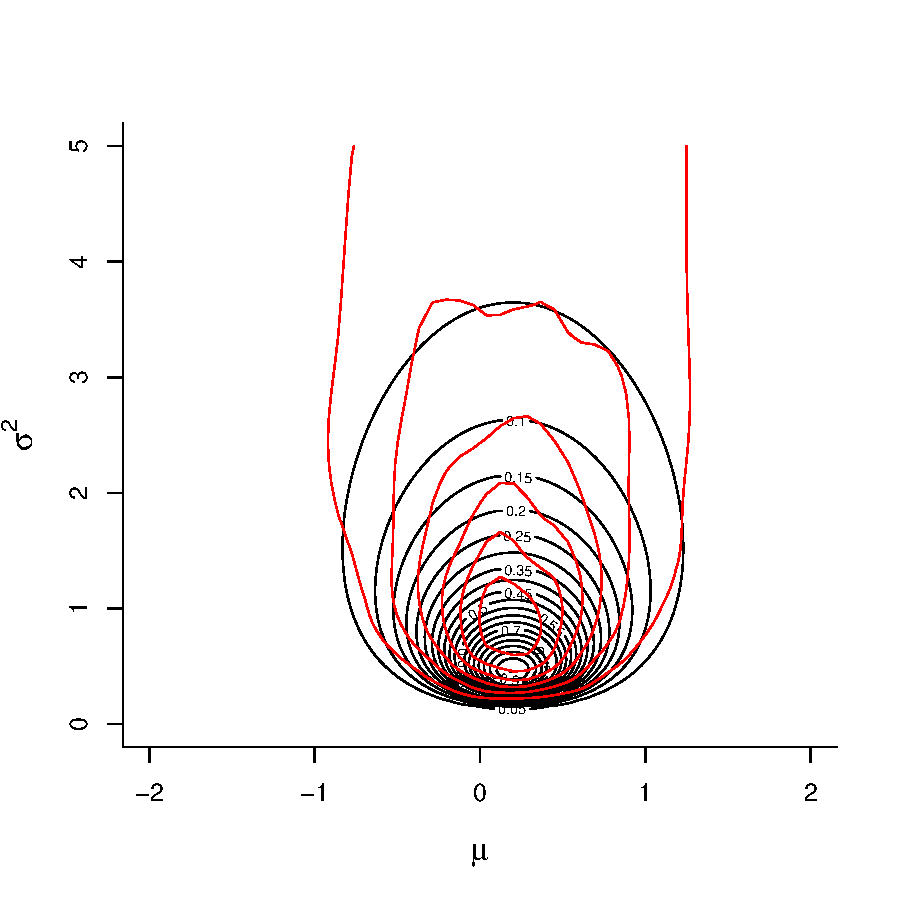
\includegraphics{Lecture1-071}
\end{center}
\caption{Likelihood surface for the likelihood $Pr({\bf y}|\mu, \sigma^{2})$ in black, and an MCMC approximation for the posterior distribution $Pr(\mu, \sigma^{2} | {\bf y})$ in red.  The likelihood has been normalised so that the maximum likelihood has a value of one, and the posterior distribution has been normalised so that the posterior mode has a value of one. A non-informative prior was used ($Pr(\mu)\sim N(0, 10^8)$ and  $Pr(\sigma^{2})\sim IW(\texttt{V}=0, \texttt{nu}=-2)$)}
\label{Psurfaceb-fig}
\end{figure}

The joint posterior mode does not coincide with either the ML or REML estimator (Figure \ref{Psurfaceb-fig}).  


but the marginal distribution of the variance component is equivalent to the REML estimator (See Figure \ref{Pmarg.NI-fig}):

\iftalk
\else
\fi

\begin{figure}[!h]
\begin{center}
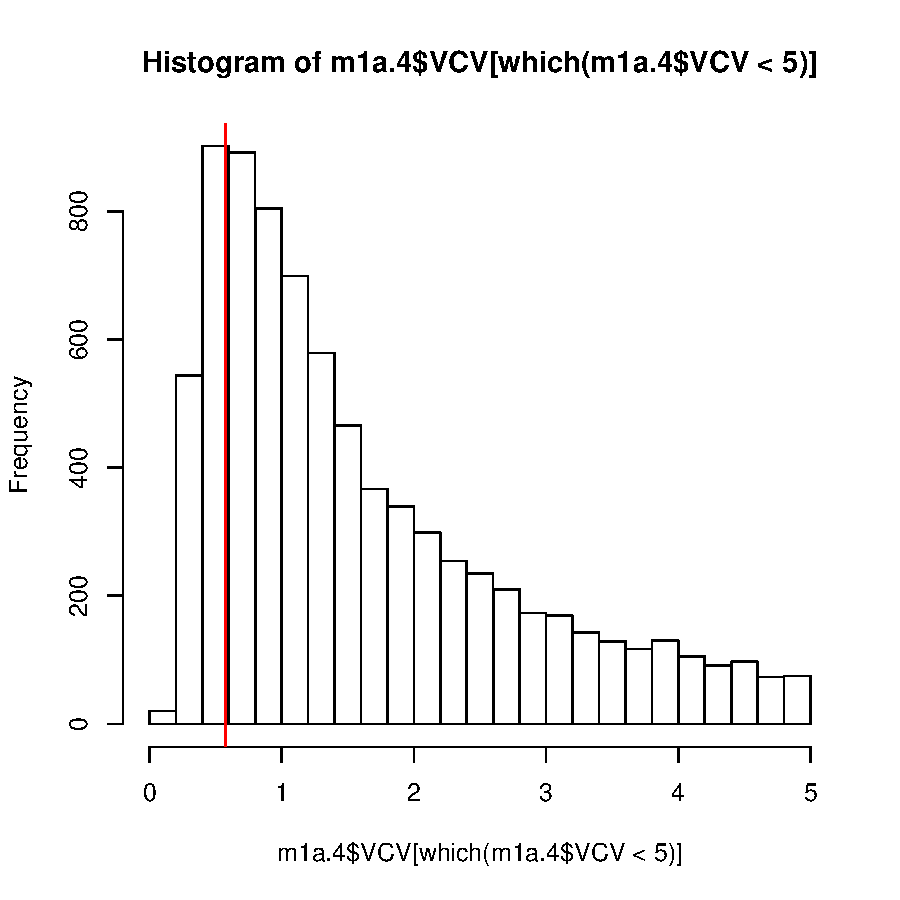
\includegraphics{Lecture1-075}
\end{center}
\caption{An MCMC approximation for the marginal posterior distribution of the variance $Pr(\sigma^{2} | {\bf y})$.  A non-informative prior specification was used ($Pr(\mu)\sim N(0, 10^8)$ and  $Pr(\sigma^{2})\sim IW(\texttt{V}=0, \texttt{nu}=-2)$) and the REML estimator of the variance (red line) coincides with the marginal posterior mode.}
\label{Pmarg.NI-fig}
\end{figure}


\ifalone
\end{document}
\else
\fi


\newif\ifalone
\alonefalse
\newif\iftalk
\talktrue

\ifalone
\documentclass{article}
\usepackage{graphicx}
\usepackage{natbib}
\usepackage{amsfonts}
\usepackage{amssymb}
\usepackage{amsthm}
\usepackage{bm}
\usepackage{Sweave}
\usepackage{lscape}
\usepackage{makeidx}
\usepackage{color}

\title{GLMs and GLMMs}

\author{Jarrod Hadfield (\texttt{j.hadfield@ed.ac.uk})}
\begin{document}
\maketitle
\else
\chapter[GLMM]{Generalised Linear Mixed Models (GLMM)}
\label{chap2}
\fi



\section{Linear Model (LM)}

A linear model is one in which unknown parameters are multiplied by observed variables and then added together to give a prediction for the response variable. As an example, lets take the results from a Swedish experiment from the sixties:

\begin{Schunk}
\begin{Sinput}
> data(Traffic)
> Traffic$year <- as.factor(Traffic$year)
> Traffic[c(1, 2, 184), ]
\end{Sinput}
\begin{Soutput}
    year day limit  y
1   1961   1    no  9
2   1961   2    no 11
184 1962  92   yes  9
\end{Soutput}
\end{Schunk}

The experiment involved enforcing speed limits on Swedish roads on some days, but on other days letting everyone drive as fast as they liked.  The response variable (\texttt{y}) was how many of their citizens were injured in road accidents! The experiment was conducted in 1961 and 1962 for 92 days in each year. As a first attempt we could specify the linear model:

\begin{Schunk}
\begin{Soutput}
y ~ limit + year + day
\end{Soutput}
\end{Schunk}

but what does this mean?\\

\subsection{Linear Predictors}

The model formula defines a set of simultaneous (linear) equations 

\begin{displaymath}
\begin{array}{cl}
E[y\texttt{[1]}] &=\beta_{1}+\beta_{2}(\texttt{limit[1]=="yes"})+\beta_{3}(\texttt{year[1]=="1962"})+\beta_{4}\texttt{day[1]}\\
E[y\texttt{[2]}] &= \beta_{1}+\beta_{2}(\texttt{limit[2]=="yes"})+\beta_{3}(\texttt{year[2]=="1962"})+\beta_{4}\texttt{day[2]}\\
\vdots&=\vdots\\
E[y\texttt{[184]}] &= \beta_{1}+\beta_{2}(\texttt{limit[184]=="yes"})+\beta_{3}(\texttt{year[184]=="1962"})+\beta_{4}\texttt{day[184]}\\
\end{array}
\label{SE-eq}
\end{displaymath}

where the $\beta$'s are the unknown coefficients to be estimated, and the variables in \texttt{this font} are observed predictors. Continuous predictors such as \texttt{day} remain unchanged, but categorical predictors are expanded into a series of binary variables of the form `\emph{do the data come from 1961, yes or no?}', `\emph{do the data come from 1962, yes or no?}', and so on for as many years for which there are data.\\ 

It is cumbersome to write out the equation for each data point in this way, and a more compact way of representing the system of equations is

\begin{equation}
E[{\bf y}] = {\bf X}{\bm \beta}
\label{lm-eq}
\end{equation}	

where ${\bf X}$ is called a design matrix and contains the predictor information, and ${\bm \beta} = [\beta_{1}\ \beta_{2}\ \beta_{3}\ \beta_{4}]^{'}$ is the vector of parameters. 

\begin{Schunk}
\begin{Sinput}
> X <- model.matrix(y ~ limit + year + day, data = Traffic)
> X[c(1, 2, 184), ]
\end{Sinput}
\begin{Soutput}
    (Intercept) limityes year1962 day
1             1        0        0   1
2             1        0        0   2
184           1        1        1  92
\end{Soutput}
\end{Schunk}

The binary predictors \emph{do the data come from 1961, yes or no?} and \emph{there was no speed limit, yes or no?} do not appear. These are the first factor levels of \texttt{year} and \texttt{limit}, and are absorbed into the global intercept ($\beta_{1}$) which is fitted by default in R.  Hence the expected number of injuries for the four combinations (on day zero) are $\beta_{1}$ for 1961 with no speed limit, $\beta_{1}+\beta_{2}$ for 1961 with a speed limit, $\beta_{1}+\beta_{3}$ for 1962 with no speed limit and  $\beta_{1}+\beta_{2}+\beta_{3}$ for 1962 with a speed limit.\\

The simultaneous equations defined by Equation (\ref{SE-eq}) cannot be solved directly because we do not know the expected value of y. We only know the observed value, which we assume is distributed around the expected value with some error. In a normal linear model we assume that these errors are normally distributed so that the data are also normally distributed (after taking into account the predictor variables):

\begin{equation}
{\bf y} = N({\bf X}{\bm \beta}, \sigma^{2}_{e}{\bf I})
\end{equation}	

${\bf I}$ is an identity matrix. It has ones along the diagonal, and zeros in the off-diagonals. The zero off-diagonals imply that the residuals are uncorrelated, and the ones along the diagonal imply that they have the same variance  $\sigma^{2}_{e}$. We could use \texttt{glm} to estimate ${\bf \beta}$ and  $\sigma^{2}_{e}$ assuming that y is normally distributed: 

\begin{Schunk}
\begin{Sinput}
> m2a.1 <- glm(y ~ limit + year + day, data = Traffic)
\end{Sinput}
\end{Schunk}

but the injuries are count data and the residuals show the typical right skew:

\iftalk
\else
\begin{Schunk}
\begin{Sinput}
> hist(m2a.1$resid)
\end{Sinput}
\end{Schunk}
\fi


\begin{figure}[!h]
\begin{center}
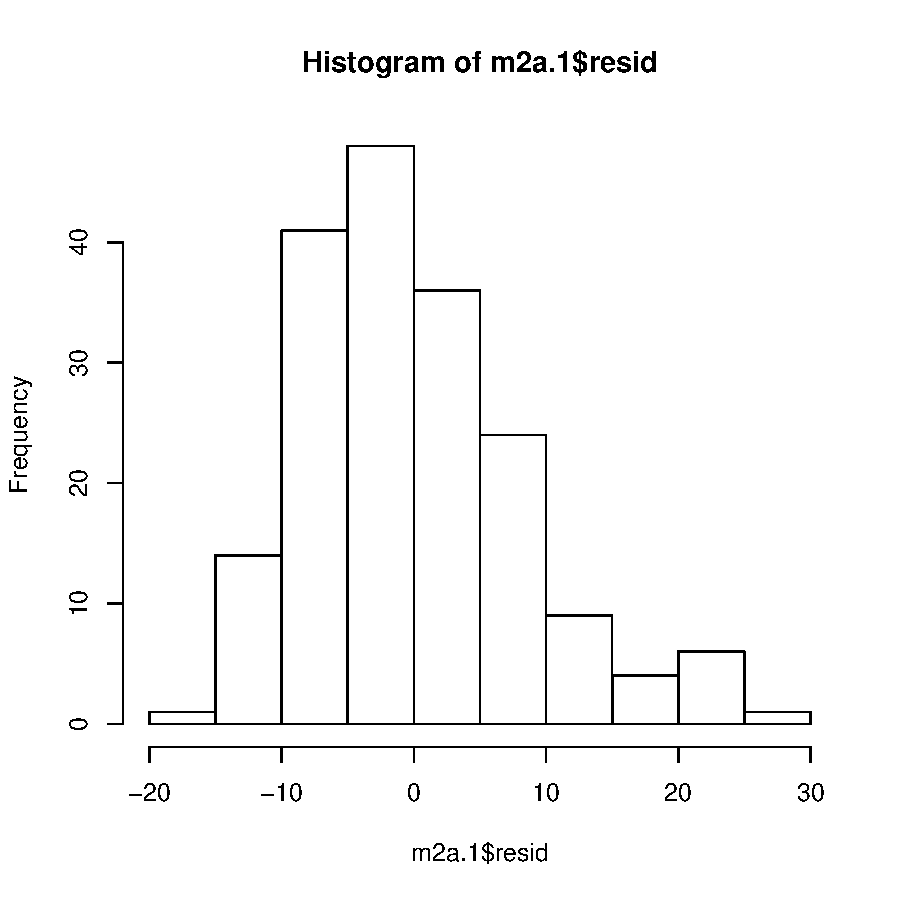
\includegraphics{Lecture2-007}
\end{center}
\caption{Histogram of residuals from model \texttt{m2a.1} which assumed they followed a Gaussian distribution.}
\label{mcmc.traffic-fig}
\end{figure}

Its not extreme, and the conclusions probably won't change, but we could assume that the data follow some other distribution.
 
\section{Generalised Linear Model (GLM)}

Generalised linear models extend the linear model to non-Gaussian data. They are essentially the same as the linear model described above, except they differ in two aspects. First, it is not necessarily the mean response that is predicted, but some function of the mean response. This function is called the link function. For example, with a log link we are trying to predict the logged expectation:

\begin{equation}
\textrm{log}(E[{\bf y}]) = {\bf X}{\bm \beta}
\end{equation}

or alternatively

\begin{equation}
E[{\bf y}] = \textrm{exp}({\bf X}{\bm \beta})
\end{equation}

where \textrm{exp} is the inverse of the log link function. The second difference is that many distributions are single parameter distributions for which a variance does not need to be estimated, because it can be inferred from the mean. For example, we could assume that the number of injuries are Poisson distributed, in which case we also make the assumption that the variance is equal to the expected value.  There are many different types of distribution and link functions and those supported by \texttt{MCMCglmm} can be found in Table \ref{dist-tab}. For now we will concentrate on a Poisson GLM with log link (the default link function for the Poisson distribution):

\begin{Schunk}
\begin{Sinput}
> m2a.2 <- glm(y ~ limit + year + day, family = poisson, data = Traffic)
> summary(m2a.2)
\end{Sinput}
\begin{Soutput}
Call:
glm(formula = y ~ limit + year + day, family = poisson, data = Traffic)

Deviance Residuals: 
    Min       1Q   Median       3Q      Max  
-4.1774  -1.4067  -0.4040   0.9725   4.9920  

Coefficients:
              Estimate Std. Error z value Pr(>|z|)    
(Intercept)  3.0467406  0.0372985  81.685  < 2e-16 ***
limityes    -0.1749337  0.0355784  -4.917 8.79e-07 ***
year1962    -0.0605503  0.0334364  -1.811   0.0702 .  
day          0.0024164  0.0005964   4.052 5.09e-05 ***
---
Signif. codes:  0 '***' 0.001 '**' 0.01 '*' 0.05 '.' 0.1 ' ' 1 

(Dispersion parameter for poisson family taken to be 1)

    Null deviance: 625.25  on 183  degrees of freedom
Residual deviance: 569.25  on 180  degrees of freedom
AIC: 1467.2

Number of Fisher Scoring iterations: 4
\end{Soutput}
\end{Schunk}

The results look fairly straightforward, having a speed limit reduces the number of injuries significantly, there are fewer injuries in 1962 (although significance is marginal) and there is a significant increase in the number of injuries over the year. Are these big effects or small effects? The coefficients are on the log scale so to get back to the data scale we need to exponentiate. The exponent of the intercept is the predicted number of injuries on day zero in 1961 without a speed limit:

\begin{Schunk}
\begin{Sinput}
> exp(m2a.2$coef["(Intercept)"])
\end{Sinput}
\begin{Soutput}
(Intercept) 
   21.04663 
\end{Soutput}
\end{Schunk}

To get the prediction for the same day with a speed limit we need to add the \texttt{limityes} coefficient

\begin{Schunk}
\begin{Sinput}
> exp(m2a.2$coef["(Intercept)"] + m2a.2$coef["limityes"])
\end{Sinput}
\begin{Soutput}
(Intercept) 
   17.66892 
\end{Soutput}
\end{Schunk}

With a speed limit there are expected to be 0.840 times less injuries than if there were no speed limits. This value can be more directly obtained:

\begin{Schunk}
\begin{Sinput}
> exp(m2a.2$coef["limityes"])
\end{Sinput}
\begin{Soutput}
 limityes 
0.8395127 
\end{Soutput}
\end{Schunk}

and holds true for any given day in either year. For example, without a speed limit on the final day of the year (92) in 1961 we expect  24.742 injuries:

\begin{Schunk}
\begin{Sinput}
> exp(m2a.2$coef["(Intercept)"] + m2a.2$coef["year1962"] + 92 * 
+     m2a.2$coef["day"])
\end{Sinput}
\begin{Soutput}
(Intercept) 
   24.74191 
\end{Soutput}
\end{Schunk}

and 20.771 injuries if a speed limit had been in place:

\begin{Schunk}
\begin{Sinput}
> exp(m2a.2$coef["(Intercept)"] + m2a.2$coef["limityes"] + m2a.2$coef["year1962"] + 
+     92 * m2a.2$coef["day"])
\end{Sinput}
\begin{Soutput}
(Intercept) 
   20.77115 
\end{Soutput}
\end{Schunk}

The proportional change is identical because the model is \emph{linear} on the log scale.

\section{Over-dispersion}  

Most count data do not conform to a Poisson distribution because the variance in the response exceeds the expectation. This is known as over-dispersion and it is easy to see how it arises, and why it is so common. In the summary to \texttt{m2a.2} note that the ratio of the residual deviance  
to the residual degrees of freedom is 3.162 which means, roughly speaking, there is 3.2 times as much variation in the residuals than what we expect.\\

If the predictor data had not been available to us then the only model we could have fitted was one with just an intercept: 

\begin{Schunk}
\begin{Sinput}
> m2a.3 <- glm(y ~ 1, data = Traffic, family = "poisson")
> summary(m2a.3)
\end{Sinput}
\begin{Soutput}
Call:
glm(formula = y ~ 1, family = "poisson", data = Traffic)

Deviance Residuals: 
    Min       1Q   Median       3Q      Max  
-3.6546  -1.4932  -0.3378   0.9284   5.0601  

Coefficients:
            Estimate Std. Error z value Pr(>|z|)    
(Intercept)  3.07033    0.01588   193.3   <2e-16 ***
---
Signif. codes:  0 '***' 0.001 '**' 0.01 '*' 0.05 '.' 0.1 ' ' 1 

(Dispersion parameter for poisson family taken to be 1)

    Null deviance: 625.25  on 183  degrees of freedom
Residual deviance: 625.25  on 183  degrees of freedom
AIC: 1517.2

Number of Fisher Scoring iterations: 4
\end{Soutput}
\end{Schunk}

for which the residual variance exceeds that expected by a factor of 3.5. Of course, the variability in the residuals must go up if there are factors that influence the number of injuries, but which we hadn't measured. Its likely that in most studies there are things that influence the response that haven't been measured, and even if each thing has small effects individually, in aggregate they can cause substantial over-dispersion.

\subsection{Multiplicative Over-dispersion}

There are two ways of dealing with over-dispersion. With \texttt{glm} the distribution name can be prefixed with \texttt{quasi} and a dispersion parameter estimated:

\begin{Schunk}
\begin{Sinput}
> m2a.4 <- glm(y ~ limit + year + day, family = quasipoisson, data = Traffic)
> summary(m2a.4)
\end{Sinput}
\begin{Soutput}
Call:
glm(formula = y ~ limit + year + day, family = quasipoisson, 
    data = Traffic)

Deviance Residuals: 
    Min       1Q   Median       3Q      Max  
-4.1774  -1.4067  -0.4040   0.9725   4.9920  

Coefficients:
             Estimate Std. Error t value Pr(>|t|)    
(Intercept)  3.046741   0.067843  44.909  < 2e-16 ***
limityes    -0.174934   0.064714  -2.703  0.00753 ** 
year1962    -0.060550   0.060818  -0.996  0.32078    
day          0.002416   0.001085   2.227  0.02716 *  
---
Signif. codes:  0 '***' 0.001 '**' 0.01 '*' 0.05 '.' 0.1 ' ' 1 

(Dispersion parameter for quasipoisson family taken to be 3.308492)

    Null deviance: 625.25  on 183  degrees of freedom
Residual deviance: 569.25  on 180  degrees of freedom
AIC: NA

Number of Fisher Scoring iterations: 4
\end{Soutput}
\end{Schunk}

\texttt{glm} uses a multiplicative model of over-dispersion and so the estimate is roughly equivalent to how many times greater the variance is than expected, after taking into account the predictor variables. You will notice that although the parameter estimates have changed very little ,the standard errors have gone up and the significance gone down. Over-dispersion, if not dealt with, can result in extreme anti-conservatism because the assumption of independence is contravened. For example, the second lowest number of accidents (8) occurred on the 91$^{st}$ day of 1961 without a speed limit. This should have been the second worst day for injuries over the whole two years, and the probability of observing 9 or less accidents on this day, under the assumption of independence is almost 1 in a 100,000:

\begin{Schunk}
\begin{Sinput}
> ppois(9, exp(m2a.2$coef["(Intercept)"] + 91 * m2a.2$coef["day"]))
\end{Sinput}
\begin{Soutput}
[1] 9.80056e-05
\end{Soutput}
\end{Schunk}

However, perhaps it was Christmas day and everything was under 5 foot of snow. Although the accidents may have been independent in the sense that all 9 cars didn't crash into each other, they are non-independent in the sense that they all happened on a day where the underlying probability may be different from that underlying any other day (data point).  

\subsection{Additive Over-dispersion}
\label{addod-sec}

I believe that a model assuming all relevant variables have been measured or controlled for, should {\bf not} be the \emph{de facto} model, and so when you specify \texttt{family=poisson} in \texttt{MCMCglmm}, over-dispersion is always dealt with\footnote{This is a bit disingenuous - it is no coincidence that the Markov chain without over-dispersion would be reducible}. However, \texttt{MCMCglmm} does not use a multiplicative model, but an additive model. 

\begin{Schunk}
\begin{Sinput}
> prior <- list(R = list(V = 1, nu = 0.002))
> m2a.5 <- MCMCglmm(y ~ limit + year + day, family = "poisson", 
+     data = Traffic, prior = prior, verbose = FALSE, pl = TRUE)
\end{Sinput}
\end{Schunk}

The element \texttt{Sol} contains the posterior distribution of the coefficients of the linear model, and we can plot their marginal distributions:


\begin{figure}[!h]
\begin{center}
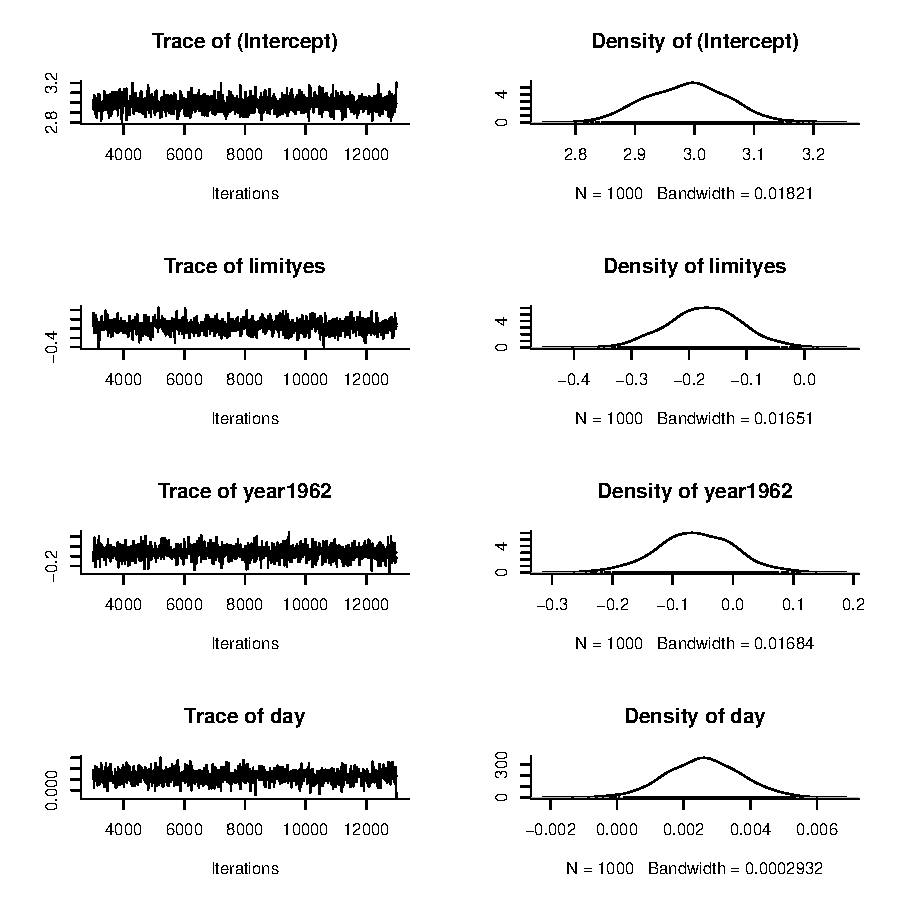
\includegraphics{Lecture2-019}
\end{center}
\caption{MCMC summary plot for the coefficients from a Poisson glm (model \texttt{m2a.5}).}
\label{mcmc.traffic-fig}
\end{figure}

Notice that the \texttt{year1962} coefficient has a high posterior density around zero, in agreement with the over-dispersed \texttt{glm} model, and that in general the estimates for the two models are broadly similar. This agreement is superficial.\\  

With additive over-dispersion the linear predictor includes a `residual', for which a residual variance is estimated (hence our prior specification). 

\begin{equation}
E[{\bf y}] = \textrm{exp}({\bf X}{\bm \beta}+{\bf e})
\end{equation}

At this point it will be handy to represent the linear model in a new way:

\begin{equation}
{\bf l} = {\bm \eta}+{\bf e}
\end{equation}

where ${\bf l}$ is a vector of latent variables ($\textrm{log}(E[{\bf y}])$ in this case) and eta (${\bm \eta}$) the usual symbol for the linear predictor (${\bf X}{\bm \beta}$). The data we observe are assumed to be Poisson variables with expectation equal to the exponentiated latent variables: 

\begin{equation}
Pois({\bf y} | \textrm{exp}({\bf l}))
\end{equation}


Note that the latent variable does not exactly predict y, as it would if the data were Gaussian, because there is additional variability in the Poisson process. In the call to \texttt{MCMCglmm} I specified \texttt{pl=TRUE} to indicate that I wanted to store the posterior distributions of latent variables. This is not usually necessary and can require a lot of memory (we have 1000 realisations for each of the 182 data points). However as an example we can obtain the residual for data point 92 which is the data from day 92 in 1961 when there was no speed limit:

\begin{Schunk}
\begin{Sinput}
> lat92 <- m2a.5$Liab[, 92]
> eta92 <- m2a.5$Sol[, "(Intercept)"] + m2a.5$Sol[, "day"] * Traffic$day[92]
> resid92 <- lat92 - eta92
> mean(resid92)
\end{Sinput}
\begin{Soutput}
[1] -0.1390523
\end{Soutput}
\end{Schunk}

This particular day has a negative residual indicating that the probability of getting injured was less than expected for this \emph{particular} realisation of that day in that year. If that \emph{particular} day could be repeated it does not necessarily mean that the actual number of injuries would always be less than expected, because it would follow a Poisson distribution with rate parameter $\lambda=$exp(\texttt{lat92})=22.039. In fact there would be a 22.549\% chance of having more injuries than if the residual had been zero:

\begin{Schunk}
\begin{Sinput}
> 1 - ppois(exp(mean(eta92)), exp(mean(lat92)))
\end{Sinput}
\begin{Soutput}
[1] 0.2254880
\end{Soutput}
\end{Schunk}

 Like residuals in a Gaussian model, the residuals are assumed to be independently and normally distributed with an expectation of zero and an estimated variance.  If the residual variance was zero then ${\bf e}$ would be a vector of zeros and the model would conform to the standard Poisson GLM. However, the posterior distribution of the residual variance is located well away form zero: 

\begin{Schunk}
\begin{Sinput}
> plot(m2a.5$VCV)
\end{Sinput}
\end{Schunk}

\begin{figure}[!h]
\begin{center}
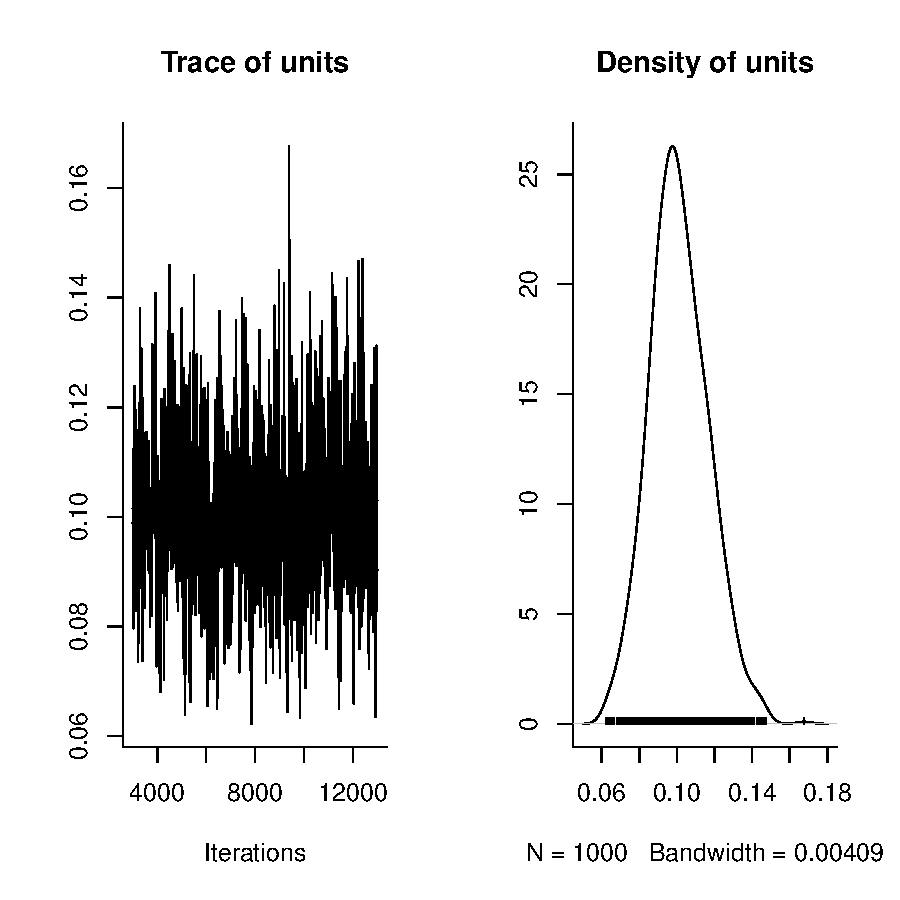
\includegraphics{Lecture2-023}
\end{center}
\caption{MCMC summary plot for the residual (\texttt{units})  variance from a Poisson glm (model \texttt{m2a.5}). The residual variance models any over-dispersion, and a residual variance of zero implies that the response conforms to a standard Poisson.}
\label{vcv.traffic-fig}
\end{figure}

The forces that created this residual were only realised on day 92 in 1961, however we could ask hypothetically what if those forces were present on another day. Figure \ref{prediction1-fig} plots the first 92 residuals as function of day (red lines) as scatter around the expectation on the log scale (solid black line). Each residual is only realised once, and the black dashed line is the hypothetical \texttt{resid92} which happened to be observed on day 92 (black circle).\\


\iftalk
\else
\fi

\iftalk
\else
\fi

\begin{figure}
\begin{minipage}[b]{0.5\linewidth} % A minipage that covers half the page
%\centering
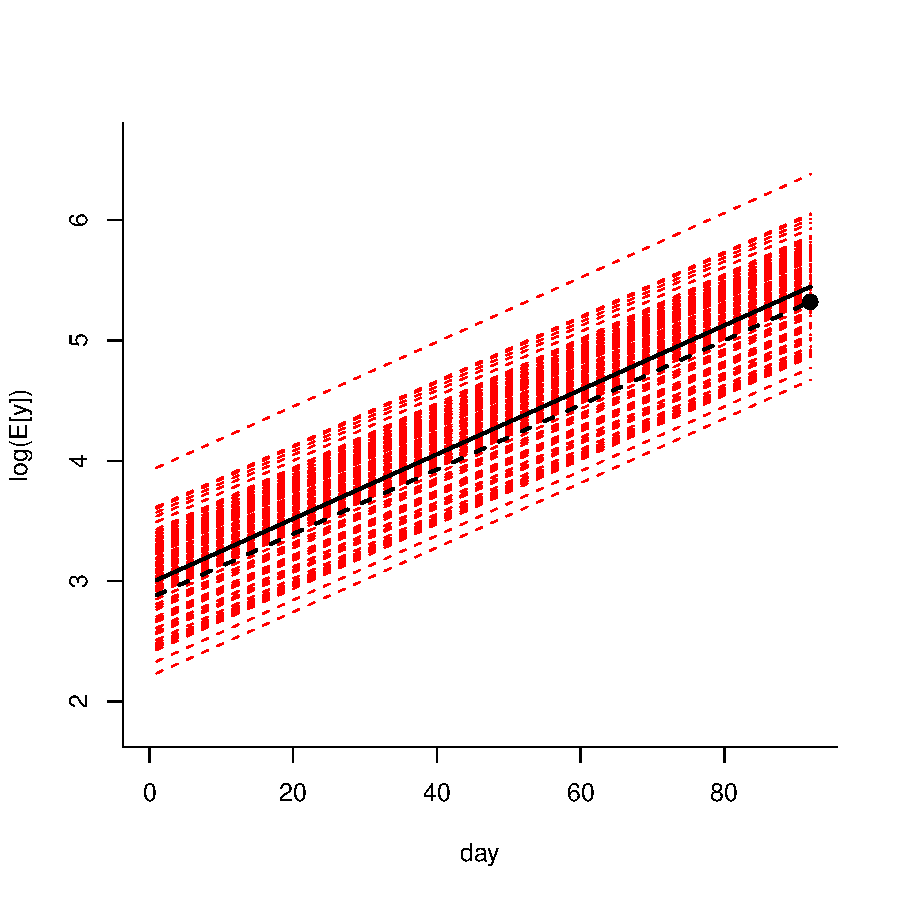
\includegraphics{Lecture2-029}
\end{minipage}
\hspace{0.2cm} % To get a little bit of space between the figures
\begin{minipage}[b]{0.5\linewidth}
%\centering
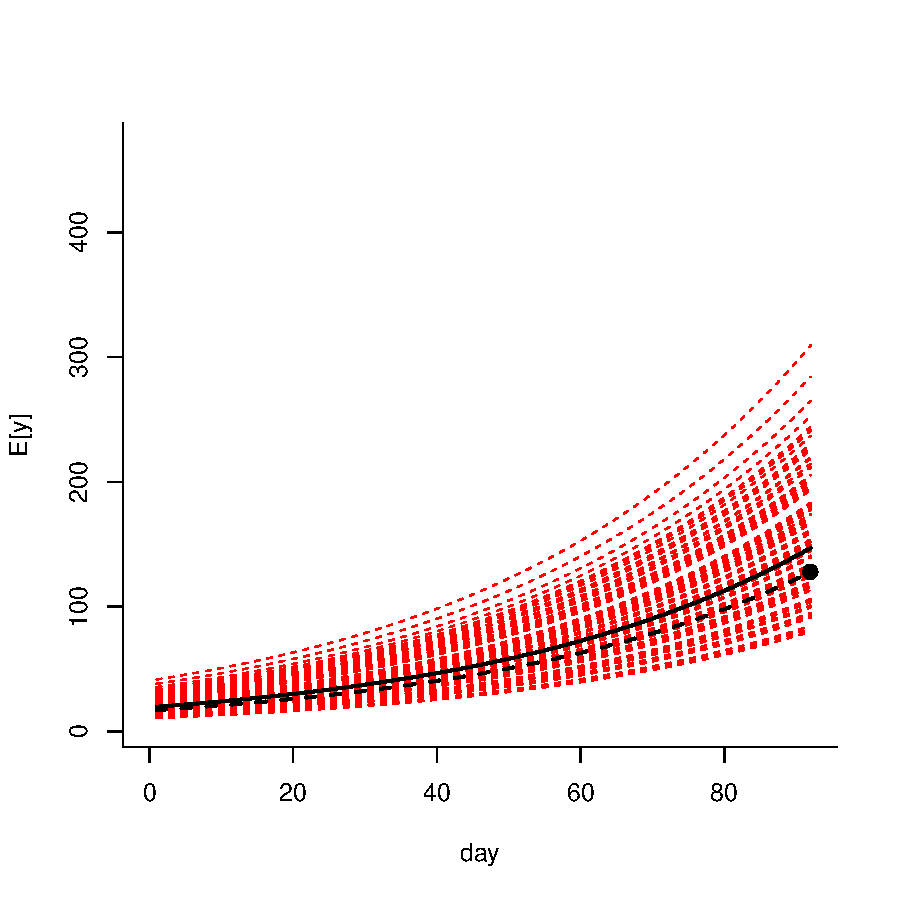
\includegraphics{Lecture2-030}
\end{minipage}
\label{prediction1-fig}
\caption{The predicted number of injuries on the log scale (left) and data scale (right) as a function of the continuous covariate \texttt{day} for 1961 without a speed limit. In order to highlight a point, the slope of the plotted relationship is an order of magnitude steeper than the model \texttt{m2a.5} estimate.The black line is the value of the linear predictor, and the red dashed lines represent noise around the linear predictor. Each dashed line is a residual from the model, which is only observed for a particular data point. The vertical distance between the black dot and the solid black line is the observed residual on day 92. The black dashed line is the predicted value of a data point observed on other days but with the same residual value.  All lines are parallel and linear on the log scale, but this is not the case on the data scale.
}
\end{figure}


It is perhaps more interesting to know the expected number of injuries that would occur on this date if we had randomly sampled one of these other residuals. To indicate an expectation taken over residuals I have subscripted expectations with $e$.  In Figure \ref{prediction3-fig}  I have plotted the distribution of the latent variables on day 92. On the log scale the expectation is simply the solid black line $\eta$. However, because the exponent function is non-linear this does not translate to the data scale and $\eta$ is actually equal to the median value on the data scale.\\ 


\iftalk
\else
\fi

\iftalk
\else
\fi

\begin{figure}
\begin{minipage}[b]{0.5\linewidth} % A minipage that covers half the page
\centering
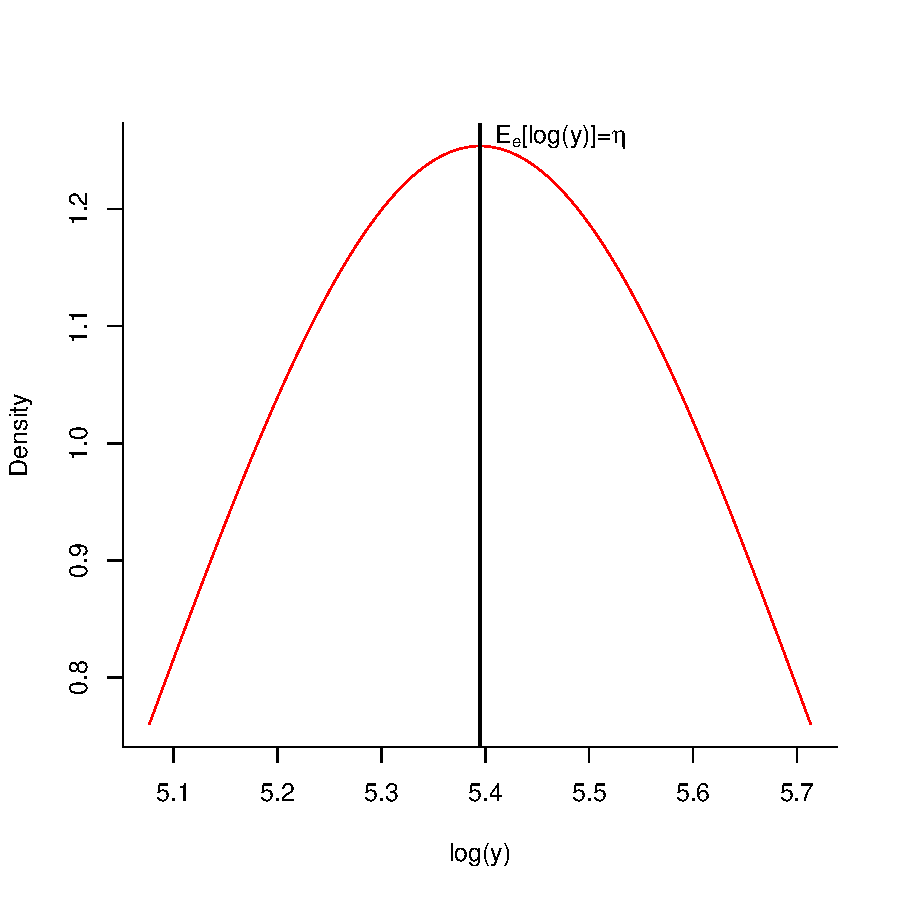
\includegraphics{Lecture2-037}
\end{minipage}
\hspace{0.5cm} % To get a little bit of space between the figures
\begin{minipage}[b]{0.5\linewidth}
\centering
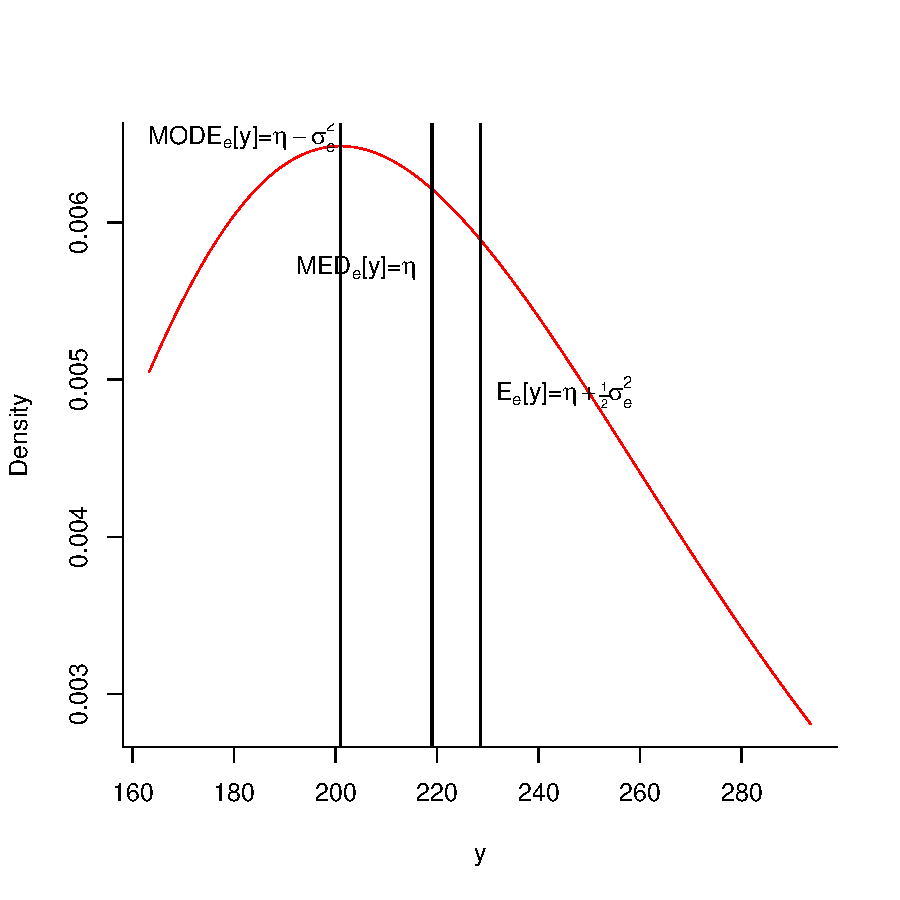
\includegraphics{Lecture2-038}
\end{minipage}
\label{prediction3-fig}
\caption{The hypothetical distribution for the number of injuries on the log scale (left) and data scale (right) for day 92 in 1961 without a speed limit. These can viewed as vertical slices from Figure \ref{prediction1-fig} on day 92. On the log scale the distribution is assumed to be normal and so the residuals are symmetrically distributed around the linear predictor. As a consequence the linear predictor ($\eta$) is equal to the mean, median and mode of the distribution on the log scale. Because the exponential function is non-linear this symmetry is lost on the data scale, and the different measures of central tendency do not coincide. Since the residuals are normal on the log scale, the distribution on the data scale is log-normal and so analytical solutions exist for the mean, mode and median.  $\sigma^{2}$ is the residual variance.
}
\end{figure}

\begin{equation}
E[{\bf y}] = \textrm{exp}({\bf X}{\bm \beta}+{\bf e})
\end{equation}


In the \texttt{Traffic} example the non linearities are small so the differences in parameter estimates are not large using either multiplicative or additive models. However, multiplying the intercept in model \texttt{m2a.5} by half the residual variance is in closer agreement with the quasipoisson model than the raw intercept:

\begin{Schunk}
\begin{Sinput}
> exp(mean(m2a.5$Sol[, "(Intercept)"] + 0.5 * m2a.5$VCV[, 1]))
\end{Sinput}
\begin{Soutput}
[1] 20.89081
\end{Soutput}
\begin{Sinput}
> exp(mean(m2a.5$Sol[, "(Intercept)"]))
\end{Sinput}
\begin{Soutput}
[1] 19.86645
\end{Soutput}
\begin{Sinput}
> exp(m2a.3$coef["(Intercept)"])
\end{Sinput}
\begin{Soutput}
(Intercept) 
   21.54891 
\end{Soutput}
\end{Schunk}

Analytical results for these transformations can be obtained for the Poisson log-normal. This is not always the case and section \ref{pred-sec} gives prediction functions for other types of distribution. One could reasonably ask, why have this additional layer of complexity, why not just stick with the multiplicative model? This brings us to random effects. 


\section{Random effects}
\label{ranef-sec}

In some cases we may have measured variables whose effects we would like to treat as random. Often the distinction between fixed and random is given by example; things like population, species, individual and vial are random, but sex, treatment and age are not. Or the distinction is made using rules of thumb; if there are few factor levels and they are interesting to other people they are fixed.  However, this doesn't really confer any understanding about what it means to treat something as fixed or random, and doesn't really allow judgements to be made regarding ambiguous variables (for example year) or give any insight into the fact that in a Bayesian analysis all effects are technically random.\\

When we treat an effect as fixed we believe that the only information regarding its value comes from data associated with that particular level. If we treat  an effect as random we also use this information, but we weight it by what other data tell us about the likely values that the effects could take. In a Bayesian analysis this additional information could come from data not formally included in the analysis, in which case it would be called a prior. In hierarchical models this additional information comes from data associated with other factor levels of the same type.\\

The degree to which this additional information is important depends on the variability of the effects, as measured by the estimated variance component, and the degree of replication within a particular level. If variability is high then most of the information must come from data associated with an individual effect, particularly if replication within that effect is high. However, if variability and replication are low then extreme mean values of the response for a given level are more likely to be due to sampling error alone, and so the estimates are shrunk towards zero.\\

It is common to hear things like `year is a random effect' as if you just have to estimate \emph{a} single effect for all years. It is also common to hear things like `years is random' as if years were sampled at random.  Better to say year effects are random and understand that it is the effects that are random not the years, and that we're trying to estimate as many effects as there are years.  In this sense they're the same as fixed effects, and we can easily treat the year effects as random to see what difference it makes.\\ 

Random effect models are often expressed as:

\begin{equation}
E[{\bf y}] = \textrm{exp}({\bf X}{\bm \beta}+{\bf Z}{\bf u}+{\bf e})
\end{equation}

where ${\bf Z}$ is a design matrix like ${\bf X}$ and ${\bf u}$ is a vector of parameters like ${\bm \beta}$. We can specify simple random effect models in the same way that we specified the fixed effects:

\begin{Schunk}
\begin{Soutput}
random =  ~ year
\end{Soutput}
\end{Schunk}

although we don't need anything to the left of the $\sim$ because the response is known from the fixed effect specification. In addition, the global intercept is suppressed by default, so in fact this specification produces the design matrix:

\begin{Schunk}
\begin{Sinput}
> Z <- model.matrix(~year - 1, data = Traffic)
> Z[c(1, 2, 184), ]
\end{Sinput}
\begin{Soutput}
    year1961 year1962
1          1        0
2          1        0
184        0        1
\end{Soutput}
\end{Schunk}

Earlier I said that there was no distinction between fixed and random effects in a Bayesian analysis - all effects are random - so lets not make the distinction and combine the design matrices (${\bf W} = [{\bf X}, {\bf Z}]$) and combine the vectors of parameters (${\bm \theta} = [{\bm \beta}^{'}, {\bf u}^{'}]^{'}$):

\begin{equation}
E[{\bf y}] = \textrm{exp}({\bf W}{\bm \theta}+{\bf e})
\label{MM-eq}
\end{equation}

If we drop year from the fixed terms, the new fixed effect design matrix looks like:

\begin{Schunk}
\begin{Sinput}
> X2 <- model.matrix(y ~ limit + day, data = Traffic)
> X2[c(1, 2, 184), ]
\end{Sinput}
\begin{Soutput}
    (Intercept) limityes day
1             1        0   1
2             1        0   2
184           1        1  92
\end{Soutput}
\end{Schunk}

and

\begin{Schunk}
\begin{Sinput}
> W <- cbind(X2, Z)
> W[c(1, 2, 184), ]
\end{Sinput}
\begin{Soutput}
    (Intercept) limityes day year1961 year1962
1             1        0   1        1        0
2             1        0   2        1        0
184           1        1  92        0        1
\end{Soutput}
\end{Schunk}

You will notice that this new design matrix is  exactly equivalent to the original design matrix \texttt{X} except we have one additional variable \texttt{year1961}. In our first model this variable was absorbed in to the global intercept because it could no be uniquely estimated from the data. What has changed that could make this additional parameter estimable?  As is usual in a Bayesian analysis, if there is no information in the data it has to come from the prior. In model \texttt{m2a.5} we used the default normal prior for the fixed effects with means of zero, large variances of $10^{8}$, and no covariances. Lets treat the year effects as random, but rather than estimate a variance component for them we'll fix the variance  at $10^{8}$ in the prior:

\begin{Schunk}
\begin{Sinput}
> prior <- list(R = list(V = 1, nu = 0.002), G = list(G1 = list(V = 1e+08, 
+     fix = 1)))
> m2a.6 <- MCMCglmm(y ~ limit + day, random = ~year, family = "poisson", 
+     data = Traffic, prior = prior, verbose = FALSE, pr = TRUE)
> plot(m2a.6$Sol)
\end{Sinput}
\end{Schunk}




\begin{figure}[!h]
\begin{center}
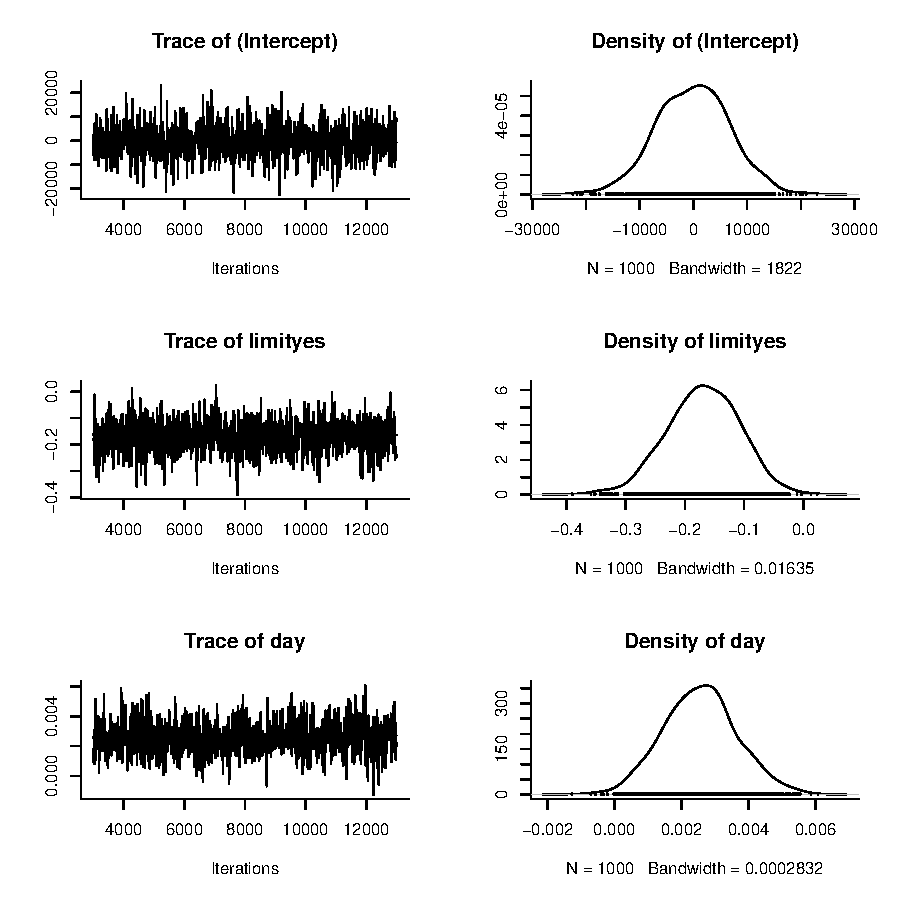
\includegraphics{Lecture2-046}
\end{center}
\caption{MCMC summary plots for the intercept, speed limit and day coefficients from model \texttt{m2a.6} where year effects were treated as random. Note the high posterior variance for the intercept.}
\label{yrandom-fig}
\end{figure}

The estimates for the intercept, day and the effect of a speed limit now appear completely different.  However, in the original model (\texttt{m2a.5}) the prediction for each year is obtained by:

\begin{Schunk}
\begin{Sinput}
> y1961.m2a.5 <- m2a.5$Sol[, "(Intercept)"]
> y1962.m2a.5 <- m2a.5$Sol[, "(Intercept)"] + m2a.5$Sol[, "year1962"]
\end{Sinput}
\end{Schunk}

However, for this model we have to add the intercept to both random effects to get the year predictions. \texttt{MCMCglmm} does not store the posterior distribution of the random effects by default, but because we specified \texttt{pr=TRUE}, the whole of ${\bm \theta}$ is stored rather than just ${\bm \beta}$:  

\begin{Schunk}
\begin{Sinput}
> y1961.m2a.6 <- m2a.6$Sol[, "(Intercept)"] + m2a.6$Sol[, "year.1961"]
> y1962.m2a.6 <- m2a.6$Sol[, "(Intercept)"] + m2a.6$Sol[, "year.1962"]
\end{Sinput}
\end{Schunk}

We can merge the two posterior distributions to see how they compare:

\begin{Schunk}
\begin{Sinput}
> y.m2a.5 <- mcmc(cbind(y1961 = y1961.m2a.5, y1962 = y1962.m2a.5))
> y.m2a.6 <- mcmc(cbind(y1961 = y1961.m2a.6, y1962 = y1962.m2a.6))
> plot(mcmc.list(y.m2a.5, y.m2a.6))
\end{Sinput}
\end{Schunk}


\begin{figure}[!h]
\begin{center}
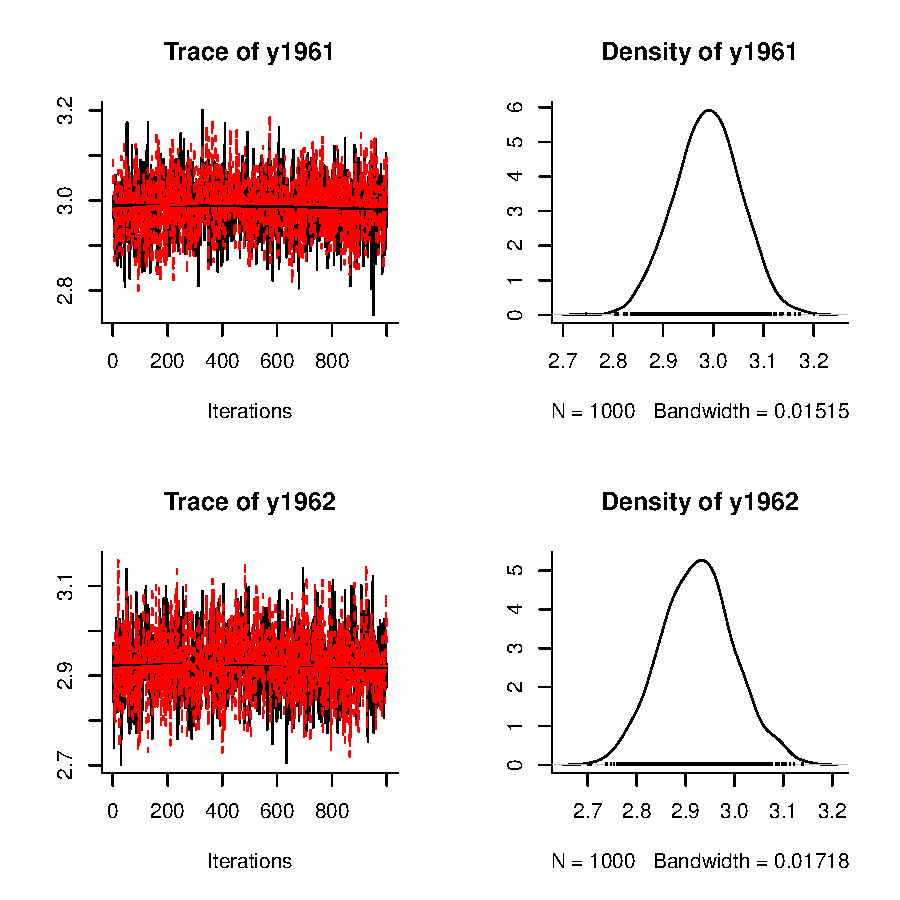
\includegraphics{Lecture2-050}
\end{center}
\caption{MCMC summary plots for the year effects from a model where year effects were treated as fixed (black) and where they were treated as random (black) but with the variance component set at a large value rather than being estimated. The posterior distributions are virtually identical.}
\label{y.pred-fig}
\end{figure}

The posterior distributions are identical (see Section \ref{PriorContr-sec}), highlighting the fact that effects that are fixed are those associated with a variance component which has been set \emph{a priori} to something large ($10^8$ in this case), where effects that are random are associated with a variance component which is not set \emph{a priori} but is estimated from the data. As the variance component tends to zero then no matter how many random effects there are, we are effectively only estimating a single parameter (the variance). This makes sense, if there were no differences between years we only need to estimate a global intercept and not separate effects for each year. Alternatively if the variance is infinite then we need to estimate separate effects for each year. In this case the intercept is confounded with the average value of the random effect, resulting in a wide marginal distribution for the intercept, and strong posterior correlations between the intercept and the mean of the random effects:

\begin{Schunk}
\begin{Sinput}
> plot(c(m2a.6$Sol[, "year.1961"] + m2a.6$Sol[, "year.1962"])/2, 
+     c(m2a.6$Sol[, "(Intercept)"]))
\end{Sinput}
\end{Schunk}


\begin{figure}[!h]
\begin{center}
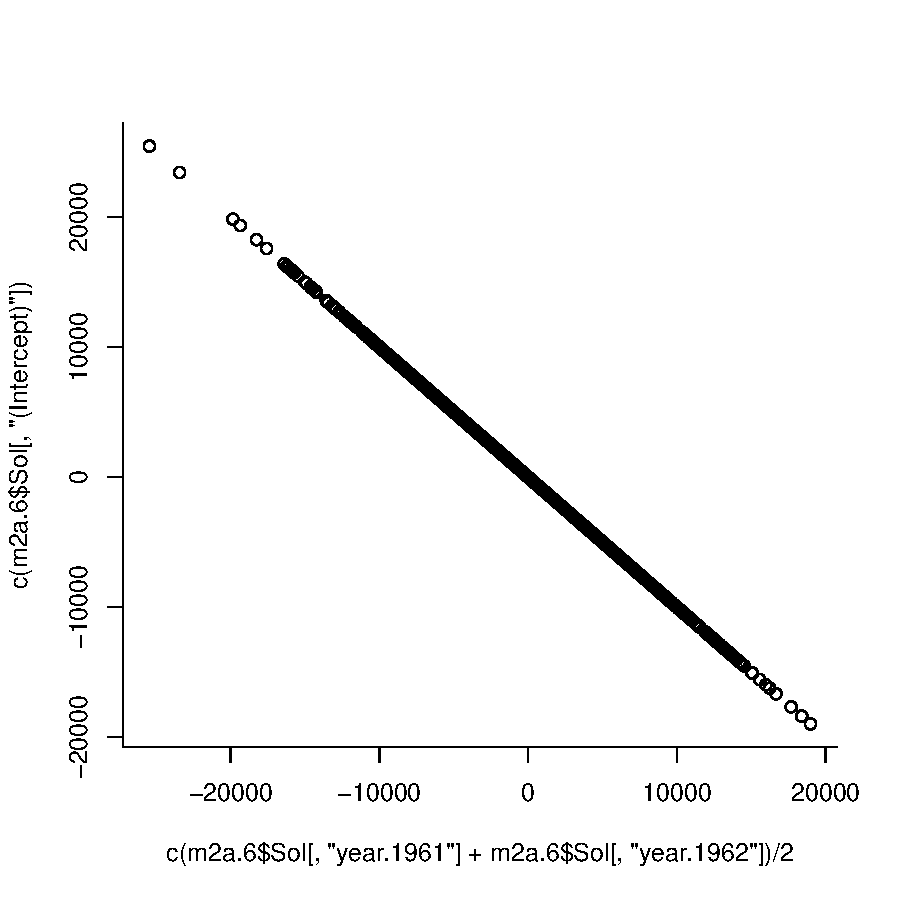
\includegraphics{Lecture2-052}
\end{center}
\caption{Joint posterior distribution of the intercept and the mean of the two random year effects. The variance component associated with year was fixed at a large value ($10^8$) and so the effects are almost completely confounded.}
\label{yfixed-fig}
\end{figure}

With only two levels, there is very little information to estimate the variance, and so we would often make the \emph{a priori} decision to treat year effects as fixed, and fix the variance components to something large (or infinity in a frequentist analysis).\\

At the moment we have day as a continuous covariate, but we could also have random day effects and ask whether the number of injuries on the same day but in different years are correlated. Rather than fixing the variance component at something large, we'll use the same weaker prior that we used for the residual variance:

\begin{Schunk}
\begin{Sinput}
> Traffic$day <- as.factor(Traffic$day)
> prior <- list(R = list(V = 1, nu = 0.002), G = list(G1 = list(V = 1, 
+     nu = 0.002)))
> m2a.7 <- MCMCglmm(y ~ year + limit + as.numeric(day), random = ~day, 
+     family = "poisson", data = Traffic, prior = prior, verbose = FALSE)
\end{Sinput}
\end{Schunk}

\texttt{day} has also gone in the fixed formula, but as a numeric variable, in order to capture any time trends in the number of injuries. Most of the over-dispersion seems to be captured by fitting day as a random term:

\begin{Schunk}
\begin{Sinput}
> plot(m2a.7$VCV)
\end{Sinput}
\end{Schunk}

\begin{figure}[!h]
\begin{center}
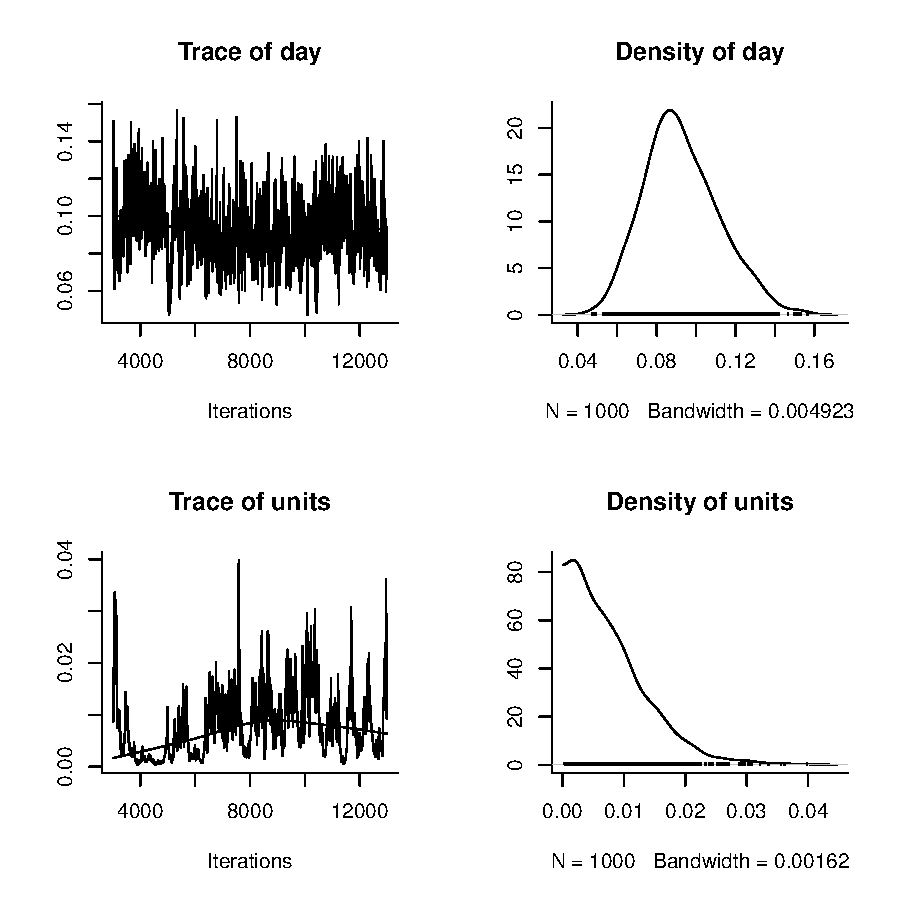
\includegraphics{Lecture2-055}
\end{center}
\caption{MCMC summary plot of the variance component associated with day (top) and the residual variance component (below). The trace for the residual variance shows strong autocorrelation and needs to be ran for longer.}
\label{GLMM.VCV-fig}
\end{figure}

In fact it explains so much that the residual variance is close to zero and mixing seems to be a problem. The chain would have to be run for longer, and the perhaps an alternative prior specification used.

\section{Prediction with Random effects}
\label{pred-sec}

In section \ref{addod-sec} we showed that for non-Gaussian data the expectation of the response variable $y$ is different from the linear predictor if we wish to average over the residuals. Often it is important to get the expectation after marginalising other random effects. For example we may not be so interested in knowing the expected number of injuries on the average day, but knowing the expected number of injuries on any random day. \\  

For the Poisson mixed model:

\begin{equation}
E[y] = \texttt{exp}({\bf X}{\bm \beta}+{\bf Z}{\bf u}+{\bf e})
\end{equation}

we can marginalise with respect to the random effects, including the over-dispersion residual:

\begin{equation}
E_{{u,e}}[y] = \textrm{exp}({\bf X}{\bm \beta}+0.5\sigma^{2})
\end{equation}

where $\sigma^{2}$ is the sum of the variance components.

For the Binomial mixed model

\begin{equation}
E[y] = \textrm{logit}^{-1}({\bf X}{\bm \beta}+{\bf Z}{\bf u}+{\bf e})
\end{equation}

it is not possible to marginilse with respect to the random effects analytically, but an approximation exists \citep[][p452]{McCulloch.2001}

\begin{equation}
E_{{u,e}}[y] = \textrm{logit}^{-1}({\bf X}{\bm \beta}-0.5\sigma^{2}\textrm{tanh}({\bf X}{\bm \beta}(1+2\textrm{exp}(-0.5\sigma^{2}))/6)))
\end{equation}

A predict function has been implemented for \texttt{MCMCglmm} although it is currently incomplete and needs further testing. However, for simpler distributions it should be OK - for example, we can predict the laibality on the latent scale after marginalising the random effects in model \texttt{m2a.7}:

\begin{Schunk}
\begin{Sinput}
> predict(m2a.7, marginal = ~day, type = "terms")[1:5]
\end{Sinput}
\begin{Soutput}
[1] 3.010650 3.013191 3.015731 3.018272 3.020812
\end{Soutput}
\end{Schunk}

or we can predict on the data scale:

\begin{Schunk}
\begin{Sinput}
> predict(m2a.7, marginal = ~day, type = "response")[1:5]
\end{Sinput}
\begin{Soutput}
[1] 22.34644 22.40141 22.45656 22.51189 22.56740
\end{Soutput}
\end{Schunk}

In addition, credible intervals can be obtained 

\begin{Schunk}
\begin{Sinput}
> predict(m2a.7, marginal = ~day, type = "response", interval = "confidence")[1:5, 
+     ]
\end{Sinput}
\begin{Soutput}
       fit      lwr      upr
1 22.34644 19.17161 25.50034
2 22.40141 19.26536 25.51614
3 22.45656 19.33657 25.51402
4 22.51189 19.43376 25.50922
5 22.56740 19.51601 25.51585
\end{Soutput}
\end{Schunk}

as can prediction intervals through posterior predictive simulation:

\begin{Schunk}
\begin{Sinput}
> predict(m2a.7, marginal = ~day, type = "response", interval = "prediction")[1:5, 
+     ]
\end{Sinput}
\begin{Soutput}
       fit      lwr      upr
1 22.35297 6.716707 41.68322
2 22.47385 5.816080 40.00978
3 22.97528 6.402591 43.04711
4 22.12104 5.890720 40.21507
5 22.16983 6.928776 42.36367
\end{Soutput}
\end{Schunk}

\section{Categorical Data}

Response variables consisting of levels of some categorical factor are best analysed using \texttt{family="categorical"} if the levels have no natural ordering,  or \texttt{family="ordinal"} if the levels do have a natural ordering, such as never $<$ sometimes $<$ always. The simplest variable of this type is binary data where the response variable is either a zero or a one, and can be analysed as \texttt{family="categorical"} (logit link) or \texttt{family="ordinal"} (probit link).   A binary distribution is a special case of the binomial distribution where the number of trials (\texttt{size}) is equal to 1. One way of interpreting a binomial response is to expand it into a series of binary variables and treat the zero's and ones as repeated measures. For example, we could generate two binomial variates each with 5 trials:

\begin{Schunk}
\begin{Sinput}
> success <- rbinom(2, size = 5, prob = c(0.4, 0.6))
> failure <- 5 - success
> binom <- rbind(success, failure)
> colnames(binom) <- c("u.1", "u.2")
> binom
\end{Sinput}
\begin{Soutput}
        u.1 u.2
success   2   5
failure   3   0
\end{Soutput}
\end{Schunk}

and then expand them into success or failure:

\begin{Schunk}
\begin{Sinput}
> binary <- matrix(rep(c(1, 0, 1, 0), binom), 1, 10)
> colnames(binary) <- rep(c("u.1", "u.2"), each = 5)
> binary
\end{Sinput}
\begin{Soutput}
     u.1 u.1 u.1 u.1 u.1 u.2 u.2 u.2 u.2 u.2
[1,]   1   1   0   0   0   1   1   1   1   1
\end{Soutput}
\end{Schunk}

We can then interpret the \texttt{units} variance in a binomial GLMM as accounting for any similarity between repeated measurements made within the same observational unit. If the binary variables within the binomial observation are correlated, this means that the underlying probability for each binomial response differs to a greater degree than can be predicted from the linear predictor. In this example the two probabilities were 0.4 and 0.6 which means that the repeated binary measures would be correlated if we only fitted the intercept (0.5).\\  

If the original data are already binary then there is no information to measure how repeatable trials are within a binomial unit because we only have a single trial per observation. This does not necessarily mean that heterogeneity in the underlying probabilities does not exist, only that we can't estimate it. Imagine we are in a room of 100 people and we are told that 5\% of the people will be dead the following day.  If the people in the room were a random sample from the UK population I would worry - \emph{I} probably have a 5\% chance of dying. If on the other hand the room was a hospital ward and I was a visitor, I may not worry too much for \emph{my} safety. The point is that in the absence of information, the binary data look the same if each person has a 5\% chance of dying or if 5 people have a 100\% chance of dying.  Most programs set the residual variance to zero and assume the former, but it is important to understand that this is a convenient but arbitrary choice. Given this, it is desirable that any conclusions drawn from the model do not depend on this arbitrary choice. Worryingly, both the location effects (fixed and random) and variance components are completely dependent on the magnitude of the residual variance.\\

To demonstrate we will use some data from a pilot study on the Indian meal moth (\emph{Plodia interpunctella}) and its granulosis virus (PiGV) collected by Hannah Tidbury \& Mike Boots at the University of Sheffield.

\begin{Schunk}
\begin{Sinput}
> data(PlodiaRB)
\end{Sinput}
\end{Schunk}

The data are taken from  874 moth pupae for which the \texttt{Pupated} variable is zero if they failed to pupate (because they were infected with the virus) or one if they successfully pupated. The 874 individuals are spread across 49 full-sib families, with family sizes ranging from 6 to 38.\\

To start we will fix the residual variance at 1:

\begin{Schunk}
\begin{Sinput}
> prior.m2b.1 = list(R = list(V = 1, fix = 1), G = list(G1 = list(V = 1, 
+     nu = 0.002)))
> m2b.1 <- MCMCglmm(Pupated ~ 1, random = ~FSfamily, family = "categorical", 
+     data = PlodiaRB, prior = prior.m2b.1, verbose = FALSE)
\end{Sinput}
\end{Schunk}

and then fit a second model where the residual variance is fixed at 2:

\begin{Schunk}
\begin{Sinput}
> prior.m2b.2 = list(R = list(V = 2, fix = 1), G = list(G1 = list(V = 1, 
+     nu = 0.002)))
> m2b.2 <- MCMCglmm(Pupated ~ 1, random = ~FSfamily, family = "categorical", 
+     data = PlodiaRB, prior = prior.m2b.2, verbose = FALSE)
\end{Sinput}
\end{Schunk}

The posterior distribution for the intercept differs between the two models (see Figure \ref{Bin1-fig}): 

\begin{Schunk}
\begin{Sinput}
> plot(mcmc.list(m2b.1$Sol, m2b.2$Sol))
\end{Sinput}
\end{Schunk}

\begin{figure}[!h]
\begin{center}
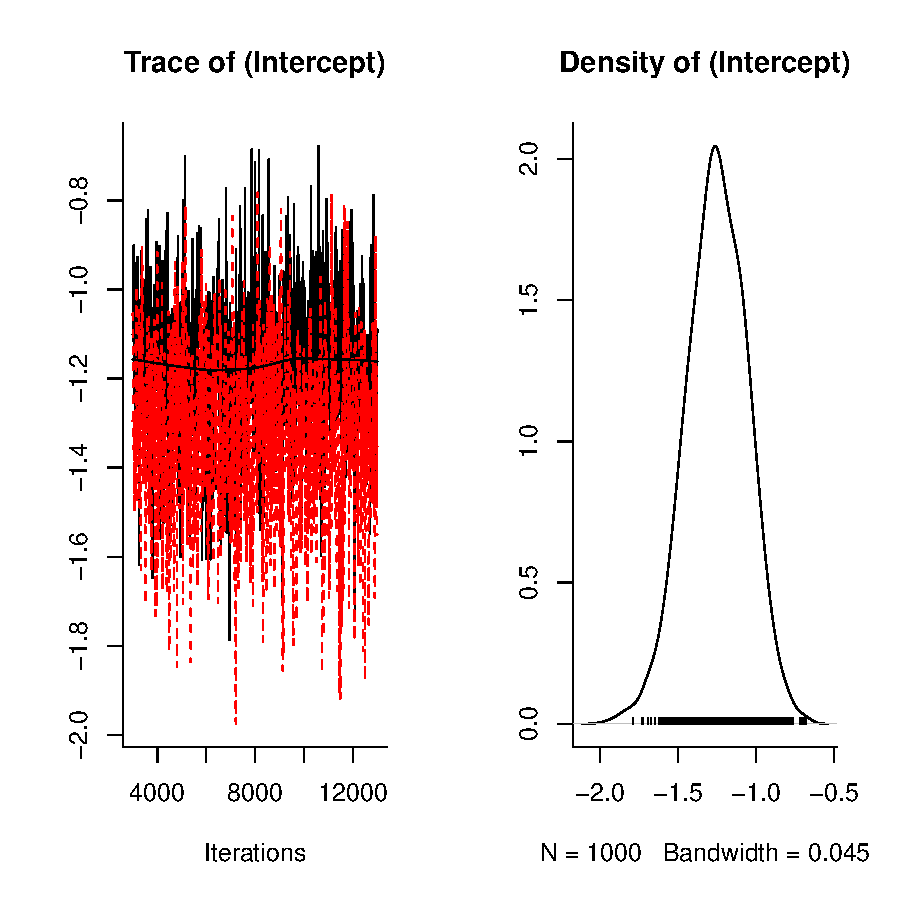
\includegraphics{Lecture2-066}
\end{center}
\caption{MCMC summary plots for the intercept of a binary GLMM where the residual variance was fixed at one (black) and two (red).}
\label{Bin1-fig}
\end{figure}

as do the variance components  (see Figure \ref{Bin2-fig}):

\begin{Schunk}
\begin{Sinput}
> plot(mcmc.list(m2b.1$VCV, m2b.2$VCV))
\end{Sinput}
\end{Schunk}

\begin{figure}[!h]
\begin{center}
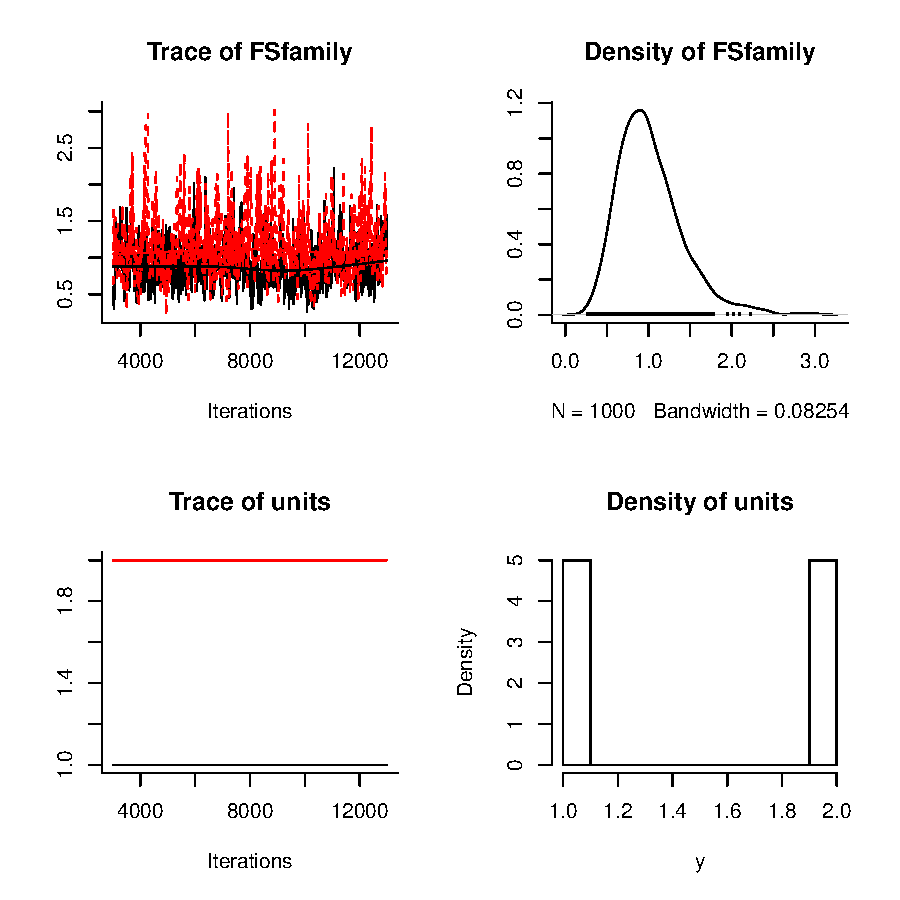
\includegraphics{Lecture2-068}
\end{center}
\caption{MCMC summary plots for the between family variance component of a binary GLMM where the residual variance was fixed at one (black) and two (red).}
\label{Bin2-fig}
\end{figure}

Should we worry? Not really. We just have to be careful about how we express the results. Stating that the family variance is 0.775 is meaningless without putting it in the context of the assumed residual variance. It is therefore more appropriate to report the intraclass correlation which in this context is the expected correlation between the state Pupated/Not Pupated, for members of the same family. It can be calculated as:

\begin{equation}
\texttt{IC} =  \frac{\sigma^{2}_{\texttt{FSfamily}}}{\sigma^{2}_{\texttt{FSfamily}}+\sigma^{2}_{\texttt{units}}+\pi^{2}/3} 
\end{equation} 

for the logit link, which is used when \texttt{family=categorical}, or 

\begin{equation}
\texttt{IC} =  \frac{\sigma^{2}_{\texttt{FSfamily}}}{\sigma^{2}_{\texttt{FSfamily}}+\sigma^{2}_{\texttt{units}}+1} 
\end{equation} 

the probit link, which is used if \texttt{family=ordinal} was specified.\\

Obtaing the posterior distribution of the intra-calss correlation for each model shows that they are sampling very similar posterior distributions (see Figure \ref{IC-fig}) 

\begin{Schunk}
\begin{Sinput}
> IC.1 <- m2b.1$VCV[, 1]/(rowSums(m2b.1$VCV) + pi^2/3)
> IC.2 <- m2b.2$VCV[, 1]/(rowSums(m2b.2$VCV) + pi^2/3)
> plot(mcmc.list(IC.1, IC.2))
\end{Sinput}
\end{Schunk}

\begin{figure}[!h]
\begin{center}
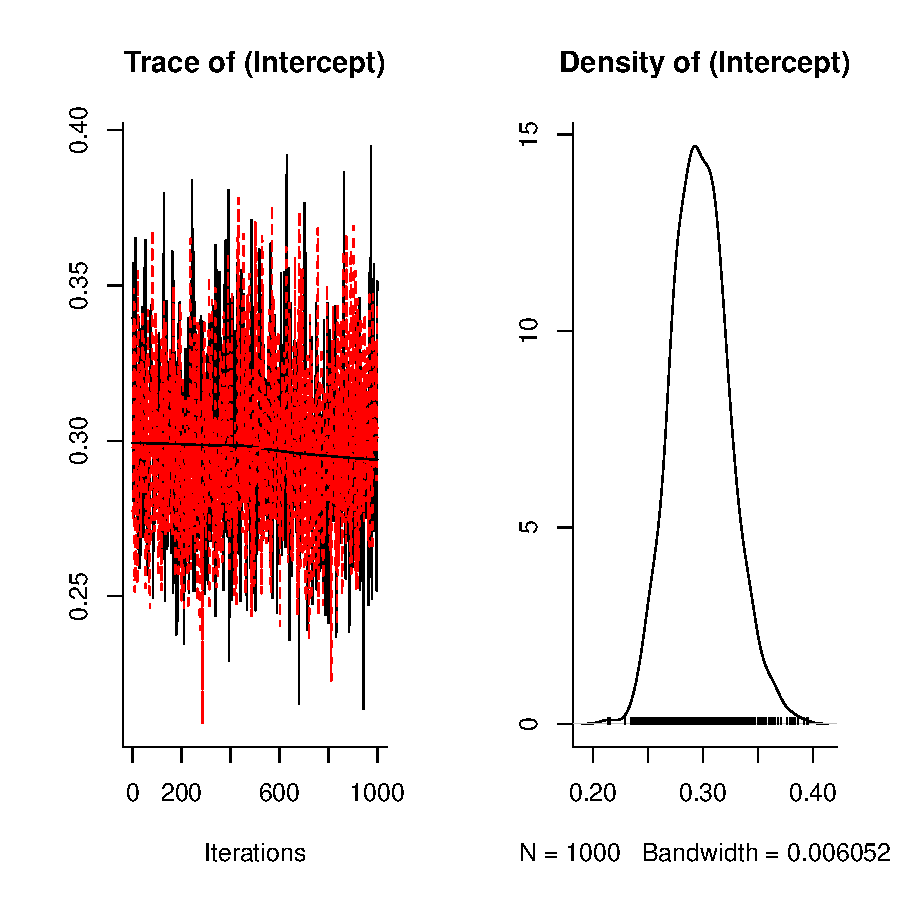
\includegraphics{Lecture2-070}
\end{center}
\caption{MCMC summary plots for the intra-family correlation from  a binary GLMM where the residual variance was fixed at one (black) and two (red).}
\label{IC-fig}
\end{figure}

Using an approximation due to \citet{Diggle.2004} we can also rescale the estimates by the estimated residual variance ($\sigma^{2}_{\texttt{units}}$) in order to obtain the posterior distributions of the parameters under the assumption that the actual residual variance ($\sigma^{2}_{e}$) is equal to some other value.  For location effects the posterior distribution needs to be multiplied by $\sqrt{\frac{1+c^{2}\sigma^{2}_{e}}{1+c^{2}\sigma^{2}_{\texttt{units}}}}$ and for the variance components the posterior distribution needs to be multiplied by $\frac{1+c^{2}\sigma^{2}_{e}}{1+c^{2}\sigma^{2}_{\texttt{units}}}$ where $c$ is some constant that depends on the link function. For the probit $c=1$ and for the logit $c=16\sqrt{3}/15\pi$. We can obtain estimates under the assumption that $\sigma^{2}_{e}=0$: 

\begin{Schunk}
\begin{Sinput}
> c2 <- ((16 * sqrt(3))/(15 * pi))^2
> Int.1 <- m2b.1$Sol/sqrt(1 + c2 * m2b.1$VCV[, 2])
> Int.2 <- m2b.2$Sol/sqrt(1 + c2 * m2b.2$VCV[, 2])
> plot(mcmc.list(as.mcmc(Int.1), as.mcmc(Int.2)))
\end{Sinput}
\end{Schunk}

\begin{figure}[!h]
\begin{center}
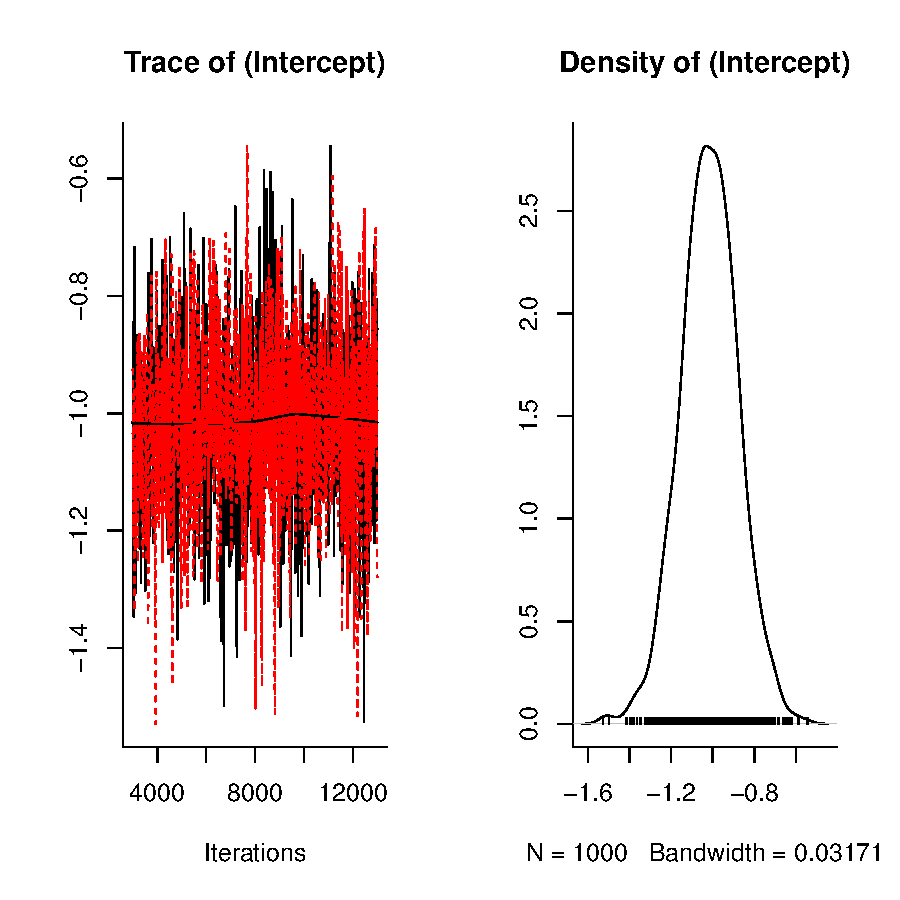
\includegraphics{Lecture2-072}
\end{center}
\caption{MCMC summary plots for the expected proportion of caterpillars pupating from  a binary GLMM where the residual variance was fixed at one (black) and two (red).}
\label{ICI-fig}
\end{figure}

The posteriors should be virtually identical under a flat prior (See Figure \ref{ICI-fig}) although with different priors this is not always the case. Remarkably, \citep{vanDyk.2001} show that leaving a diffuse prior on $\sigma^{2}_{\texttt{units}}$ and rescaling the estimates each iteration, a Markov chain with superior mixing and convergence properties can be obtained (See section \ref{secPX}).\\  

It should also be noted that a diffuse prior on the logit scale is not necessarily weakly informative on the probability scale. For example, the default setting for the prior on the intercept is $N(0, 10^{8})$ on the logit scale, which although relatively flat across most of the probability scale, has a lot of density close to zero and one:


\begin{Schunk}
\begin{Sinput}
> hist(plogis(rnorm(1000, 0, sqrt(1e+08))))
\end{Sinput}
\end{Schunk}

\begin{figure}[!h]
\begin{center}
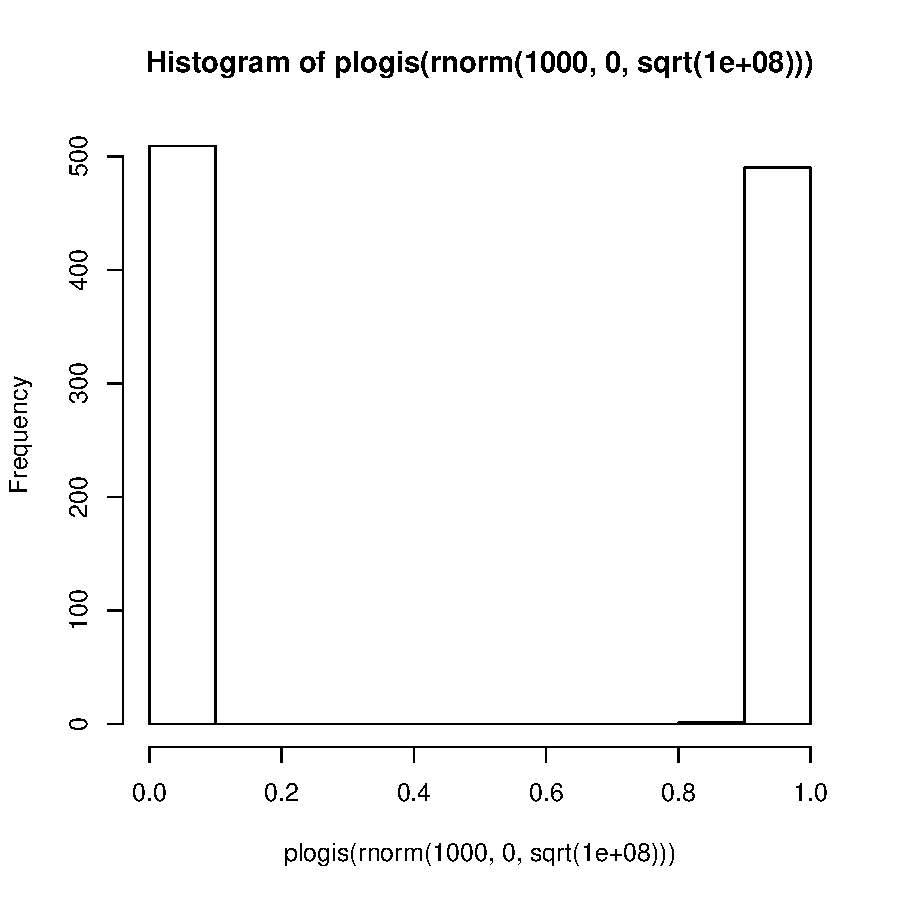
\includegraphics{Lecture2-074}
\end{center}
\caption{Histogram of 1000 random deviates from a normal distribution with a mean of zero and a large variance ($10^8$) after undergoing an inverse logit transformation.}
\label{invlogit-fig}
\end{figure}

This diffuse prior can cause problems if there is complete (or near complete) separation. Generally this happens when the binary data associated with some categorical data are all success or all failures. For example, imagine we had 50 binary observations from an experiment with two treatments, for the first treatment the probability of success is 0.5 but in the second it is only one in a thousand:

\begin{Schunk}
\begin{Sinput}
> treatment <- gl(2, 25)
> y <- rbinom(50, 1, c(0.5, 0.001)[treatment])
> data.bin <- data.frame(treatment = treatment, y = y)
> table(data.bin)
\end{Sinput}
\begin{Soutput}
         y
treatment  0  1
        1 17  8
        2 25  0
\end{Soutput}
\end{Schunk}
 
if we analyse using \texttt{glm} we see some odd behaviour:

\begin{Schunk}
\begin{Sinput}
> m2c.1 <- glm(y ~ treatment, data = data.bin, family = "binomial")
> summary(m2c.1)
\end{Sinput}
\begin{Soutput}
Call:
glm(formula = y ~ treatment, family = "binomial", data = data.bin)

Deviance Residuals: 
       Min          1Q      Median          3Q         Max  
-8.783e-01  -8.783e-01  -7.976e-05  -7.976e-05   1.510e+00  

Coefficients:
             Estimate Std. Error z value Pr(>|z|)  
(Intercept)   -0.7538     0.4287  -1.758   0.0787 .
treatment2   -18.8123  2150.8026  -0.009   0.9930  
---
Signif. codes:  0 '***' 0.001 '**' 0.01 '*' 0.05 '.' 0.1 ' ' 1 

(Dispersion parameter for binomial family taken to be 1)

    Null deviance: 43.967  on 49  degrees of freedom
Residual deviance: 31.343  on 48  degrees of freedom
AIC: 35.343

Number of Fisher Scoring iterations: 18
\end{Soutput}
\end{Schunk}

the effect of treatment does not appear significant despite the large effect size. This is in direct contrast to an exact binomial test: 

\begin{Schunk}
\begin{Sinput}
> m2c.2 <- binom.test(table(data.bin)[2, 2], 25)
> m2c.2
\end{Sinput}
\begin{Soutput}
	Exact binomial test

data:  table(data.bin)[2, 2] and 25 
number of successes = 0, number of trials = 25, p-value = 5.96e-08
alternative hypothesis: true probability of success is not equal to 0.5 
95 percent confidence interval:
 0.0000000 0.1371852 
sample estimates:
probability of success 
                     0 
\end{Soutput}
\end{Schunk}

where the  95\% confidence interval for the probability of success is  0.000 to 0.137.\\

The default \texttt{MCMCglmm} model also behaves oddly (see Figure \ref{separation1-fig}):

\begin{Schunk}
\begin{Sinput}
> prior.m2c.3 = list(R = list(V = 1, fix = 1), G = list(G1 = list(V = 1, 
+     nu = 0.002)))
> m2c.3 <- MCMCglmm(y ~ treatment, data = data.bin, family = "categorical", 
+     prior = prior.m2c.3, verbose = FALSE)
> plot(m2c.3$Sol)
\end{Sinput}
\end{Schunk}



\begin{figure}[!h]
\begin{center}
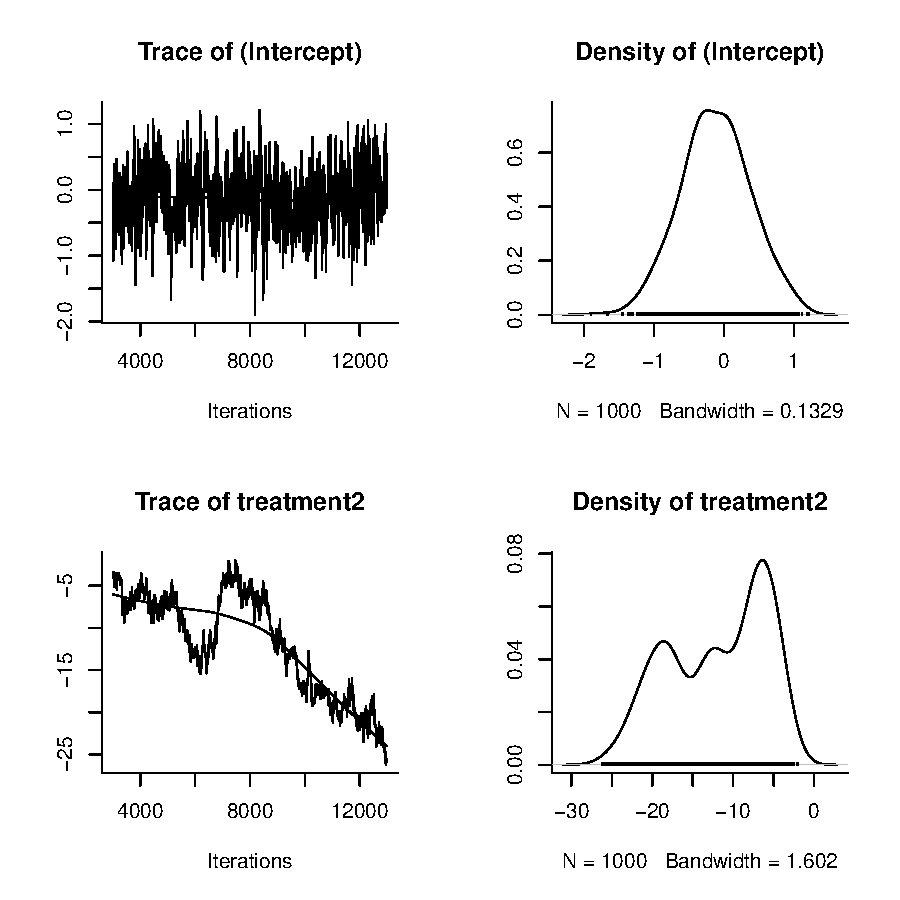
\includegraphics{Lecture2-081}
\end{center}
\caption{MCMC summary plots for the intercept and treatment effect in a binary GLM. In treatment 2 all 25 observations were failures and so the ML estimator on the probability scale is zero and $-\infty$ on the logit scale. With a flat prior on the treatment effect the posterior distribution is improper, and with a diffuse prior (as used here) the posterior is dominated by the high prior densities at extreme values.}
\label{separation1-fig}
\end{figure}

For these types of problems, I usually remove the global intercept (\texttt{-1}) and use the prior $N(0, \sigma^{2}_{\texttt{units}}+\pi^2/3)$ because this is reasonably flat on the probability scale when a logit link is used. For example,

\begin{Schunk}
\begin{Sinput}
> prior.m2c.4 = list(B = list(mu = c(0, 0), V = diag(2) * (1 + 
+     pi^2/3)), R = list(V = 1, fix = 1), G = list(G1 = list(V = 1, 
+     nu = 0.002)))
> m2c.4 <- MCMCglmm(y ~ treatment - 1, data = data.bin, family = "categorical", 
+     prior = prior.m2c.4, verbose = FALSE)
> plot(m2c.4$Sol)
\end{Sinput}
\end{Schunk}


looks a little better (see Figure \ref{separation1-fig}), and the posterior distribution for the probability of success in treatment 2 is consistent with the exact binomial test for which the 95\% CI were (0.000 - 0.137). With such a simple model, the prediction for observation 26 is equal to the  treatment 2 effect and so we can get the the credible interval (on the data scale) for treatment 2 using the predict function:




\begin{figure}[!h]
\begin{center}
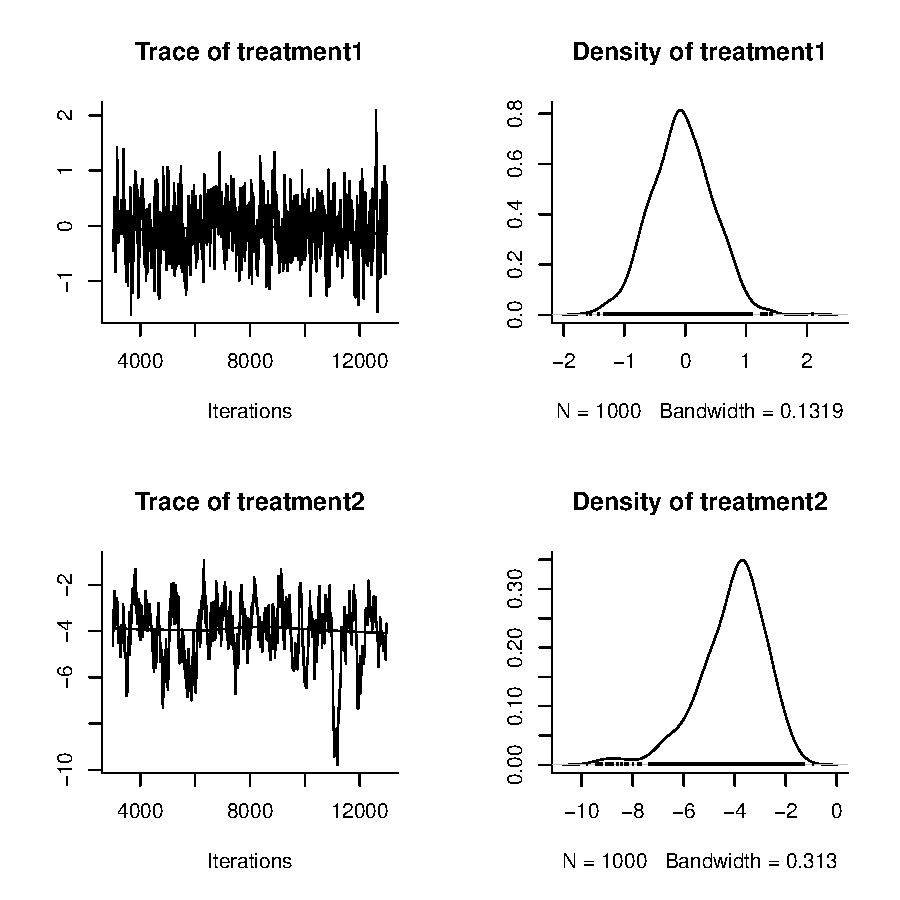
\includegraphics{Lecture2-085}
\end{center}
\caption{MCMC summary plots for the intercept and treatment effect in a binary GLM. In treatment 2 all 25 observations were failures and so the ML estimator on the probability scale is zero and $-\infty$ on the logit scale. A flat prior on the probability scale was used and the posterior distribution is better behaved than if a flat prior on the logit scale had been used (see Figure \ref{separation1-fig}).}
\label{separation2-fig}
\end{figure}

\begin{Schunk}
\begin{Sinput}
> predict(m2c.4, interval = "confidence")[26, ]
\end{Sinput}
\begin{Soutput}
        fit         lwr         upr 
0.038639512 0.001035282 0.095372019 
\end{Soutput}
\end{Schunk}


\section{A note on fixed effect priors and covariances}
\label{PriorContr-sec}

Fixed and random effects are essentially the same thing. The only difference is that the variance component for the fixed effects is usually fixed at some large value, whereas the variance component for the random effects is estimated.  In section \ref{ranef-sec} I demonstrated this by claiming that a model where year effects were fixed (\texttt{m2a.5}) was identical to one where they were treated as random, but with the variance component set to a large value (\texttt{m2a.6}). This was a white lie as I did not want to distract attention from the main point. The reason why they were not identical is as follows:\\

In the fixed effect model we had the prior:  

\begin{equation}
\begin{array}{rcl}
\left[
\begin{array}{c}
 \beta_{\texttt{(Intercept)}}\\
 \beta_{\texttt{year1962}}\\
\end{array}
\right]
\sim
&
\left[
\begin{array}{cc}
10^8&0\\
0&10^8\\
\end{array}
\right]\\
\end{array}
\end{equation}

Where $\beta_{\texttt{(Intercept)}}$ and $\beta_{\texttt{year1962}}$ are the fixed effects to be estimated.\\

Remembering the identity  $\sigma^{2}_{(a+b)} = \sigma^{2}_{a}+ \sigma^{2}_{b}+\sigma_{a,b}$, this implies:

\begin{equation}
\begin{array}{rccl}
\left[
\begin{array}{c}
 \beta_{1961}\\
 \beta_{1962}\\
\end{array}
\right]
=
&
\left[
\begin{array}{c}
 \beta_{\texttt{(Intercept)}}\\
 \beta_{\texttt{(Intercept)}}+\beta_{\texttt{year1962}}\\
\end{array}
\right]
\sim
&
\left[
\begin{array}{cc}
10^8&10^8\\
10^8&10^8+10^8\\
\end{array}
\right]
&=
\left[
\begin{array}{cc}
10^8&10^8\\
10^8&20^8\\
\end{array}
\right]\\
\end{array}
\end{equation}

where $\beta_{1961}$ and $\beta_{1962}$ are the actual year effects, rather than the global intercept and the contrast. In hindsight this is a bit odd, for one thing we expect the 1962 effect to be twice as variable as the 1961 effect. With such weak priors it makes little difference, but lets reparameterise the model anyway.\\

 Rather than having a global intercept and a year contrast, we will have separate intercepts for each year:

\begin{Schunk}
\begin{Sinput}
> X3 <- model.matrix(y ~ year - 1, data = Traffic)
> X3[c(1, 2, 184), ]
\end{Sinput}
\begin{Soutput}
    year1961 year1962
1          1        0
2          1        0
184        0        1
\end{Soutput}
\end{Schunk}

and a prior that has a covariance between the two year effects:

\begin{Schunk}
\begin{Sinput}
> PBV.yfixed <- diag(2) * 1e+08
> PBV.yfixed[1, 2] <- PBV.yfixed[2, 1] <- 1e+08/2
> PBV.yfixed
\end{Sinput}
\begin{Soutput}
      [,1]  [,2]
[1,] 1e+08 5e+07
[2,] 5e+07 1e+08
\end{Soutput}
\begin{Sinput}
> prior.m2a.5.1 <- list(B = list(mu = rep(0, 2), V = PBV.yfixed), 
+     R = list(V = 1, nu = 0.002))
\end{Sinput}
\end{Schunk}

This new model:

\begin{Schunk}
\begin{Sinput}
> m2a.5.1 <- MCMCglmm(y ~ year - 1, family = "poisson", data = Traffic, 
+     prior = prior.m2a.5.1, verbose = FALSE)
\end{Sinput}
\end{Schunk}

has the same form as a mixed effect model with a prior variance of $\frac{10^{8}}{2}$ for the intercept, and the variance component associated with the random year effects also fixed at $\frac{10^{8}}{2}$:

\begin{Schunk}
\begin{Sinput}
> prior.m2a.6.1 <- list(B = list(mu = 0, V = 1e+08/2), R = list(V = 1, 
+     nu = 0.002), G = list(G1 = list(V = 1e+08/2, fix = 1)))
\end{Sinput}
\end{Schunk}


This arises because the two random effects have the joint prior distribution:

\begin{equation}
\begin{array}{rl}
\left[
\begin{array}{c}
 \beta_{\texttt{year.1961}}\\
 \beta_{\texttt{year.1962}}\\
\end{array}
\right]
\sim
&
\left[
\begin{array}{cc}
\frac{10^{8}}{2}&0\\
0&\frac{10^{8}}{2}\\
\end{array}
\right]\\
\end{array}
\end{equation}

which when combined with the prior for the intercept, $N(0, \frac{10^{8}}{2})$, gives:

\begin{equation}
\begin{array}{rccl}
\left[
\begin{array}{c}
 \beta_{1961}\\
 \beta_{1962}\\
\end{array}
\right]
=
&
\left[
\begin{array}{c}
 \beta_{\texttt{(Intercept)}}+\beta_{\texttt{year.1961}}\\
 \beta_{\texttt{(Intercept)}}+\beta_{\texttt{year.1962}}\\
\end{array}
\right]
\sim
&
\left[
\begin{array}{cc}
\frac{10^{8}}{2}+\frac{10^{8}}{2}&\frac{10^{8}}{2}\\
\frac{10^{8}}{2}&\frac{10^{8}}{2}+\frac{10^{8}}{2}\\
\end{array}
\right]
&=
\left[
\begin{array}{cc}
10^8&\frac{10^{8}}{2}\\
\frac{10^{8}}{2}&10^8\\
\end{array}
\right]
\\
\end{array}
\end{equation}

which is equivalent to the \texttt{PBV.yfixed} parameteristaion of for the two years.\\

The model:

\begin{Schunk}
\begin{Sinput}
> m2a.6.1 <- MCMCglmm(y ~ 1, random = ~year, family = "poisson", 
+     data = Traffic, prior = prior.m2a.6.1, verbose = FALSE, pr = TRUE)
\end{Sinput}
\end{Schunk}

is therefore sampling from the same posterior distribution as model \texttt{m2a.5.1}.
\ifalone
\end{document}
\else
\fi




\newif\ifalone
\alonefalse
\newif\iftalk
\talktrue



\ifalone
\documentclass{article}
\usepackage{graphicx}
\usepackage{natbib}
\usepackage{amsfonts}
\usepackage{amssymb}
\usepackage{amsthm}
\usepackage{bm}
\usepackage{Sweave}
\usepackage{lscape}
\usepackage{makeidx}
\usepackage{color}
\usepackage{longtable}

\title{Categorical Random Interactions}

\author{Jarrod Hadfield (\texttt{j.hadfield@ed.ac.uk})}
\begin{document}
\maketitle
\else
\chapter{Categorical Random Interactions}
\label{chap3}
\fi




Random effect specification is a common cause of confusion, especially when we want to form interactions in the random terms. To illustrate the possibilities we'll use data collected on Blue tits.

\begin{Schunk}
\begin{Sinput}
> data(BTdata)
\end{Sinput}
\end{Schunk}

The data are morphological measurements (\texttt{tarsus} length and \texttt{back} colour) made on 828 blue tit chicks from 106 mothers (\texttt{dam}). Half the offspring from each mother were swapped with half the offspring from another mother soon after hatching. The nest they were reared in is recorded as \texttt{fosternest}.  

\begin{Schunk}
\begin{Sinput}
> prior = list(R = list(V = 1, nu = 0.002), G = list(G1 = list(V = 1, 
+     nu = 0.002), G2 = list(V = 1, nu = 0.002)))
> m3a.1 <- MCMCglmm(tarsus ~ sex, random = ~dam + 
+     fosternest, data = BTdata, verbose = FALSE, 
+     prior = prior)
\end{Sinput}
\end{Schunk}

fits \texttt{sex} as a fixed effect, and \texttt{dam} and \texttt{fosternest} as random effects.  

\begin{Schunk}
\begin{Sinput}
> diag(autocorr(m3a.1$VCV)[2, , ])
\end{Sinput}
\begin{Soutput}
        dam  fosternest       units 
 0.11102705  0.30977997 -0.02760598 
\end{Soutput}
\begin{Sinput}
> plot(m3a.1$VCV)
\end{Sinput}
\end{Schunk}

\begin{figure}[!h]
\begin{center}
\begin{Schunk}
\begin{Soutput}
        dam  fosternest       units 
 0.11102705  0.30977997 -0.02760598 
\end{Soutput}
\end{Schunk}
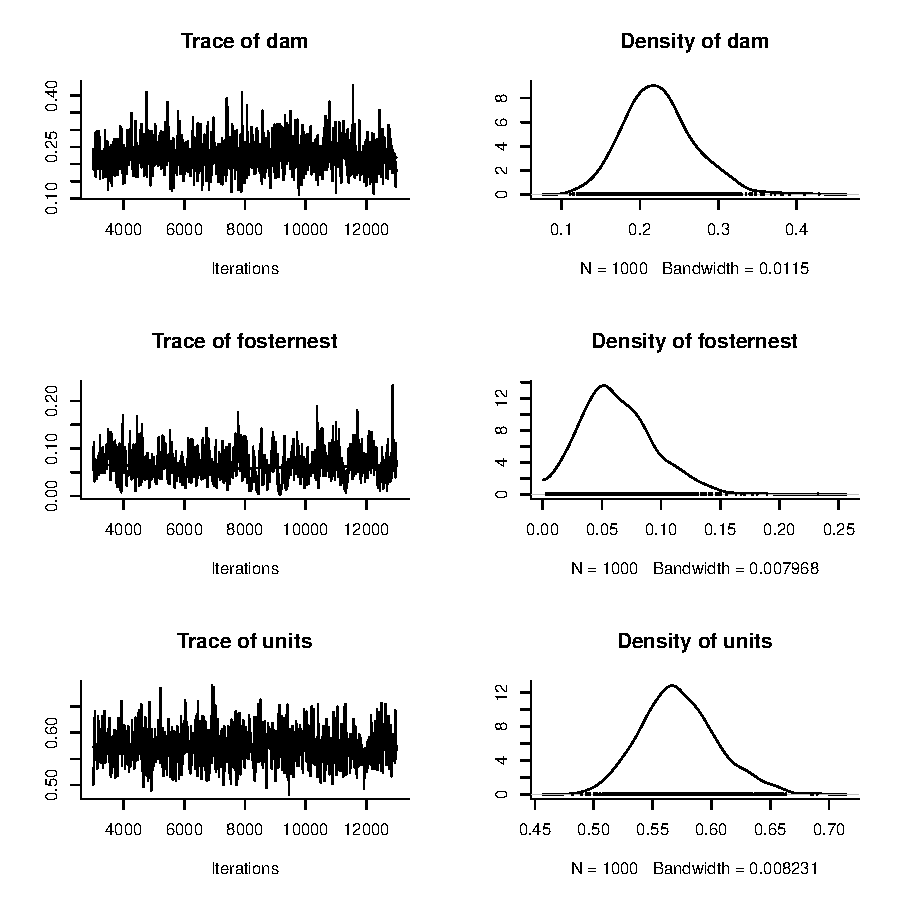
\includegraphics{Lecture3-005}
\end{center}
\caption{MCMC summary plot for the variance components from model \texttt{m3a.1}.}
\label{mBTVCV-fig}
\end{figure}

Perhaps the autocorrelation for the \texttt{fosternest} variance is a little higher than we would like, and so we may like to run it for longer.

\begin{Schunk}
\begin{Sinput}
> effectiveSize(m3a.1$VCV)
\end{Sinput}
\begin{Soutput}
       dam fosternest      units 
  799.3353   472.3695  1000.0000 
\end{Soutput}
\end{Schunk}

Indeed, we've only sampled the fosternest variance about half as well as the other two variance components.\\

The posterior correlation between the parameters is low

\begin{Schunk}
\begin{Sinput}
> cor(m3a.1$VCV)
\end{Sinput}
\begin{Soutput}
                   dam fosternest       units
dam         1.00000000 -0.1831774 -0.03579065
fosternest -0.18317736  1.0000000 -0.16361545
units      -0.03579065 -0.1636154  1.00000000
\end{Soutput}
\end{Schunk}

which is not that surprising give the data come from an experiment which was designed in order to estimate these variance components. In general, variance components will show negative posterior correlations because the the total variance is being divided up. Imagine cutting a piece of string; making one bit longer has to reduce the size of the other bits, by necessity. If we hadn't experimentally manipulated the birds then all chicks with the same mother, would be raised in the same nest, and there would be no information in the data to separate these terms. In this case the posterior correlation between these parameters would approach -1 as the prior information goes to zero.\\  

The lower 95\% credible interval for the \texttt{fosternest} variance is low

\begin{Schunk}
\begin{Sinput}
> HPDinterval(m3a.1$VCV)
\end{Sinput}
\begin{Soutput}
                lower     upper
dam        0.13766735 0.3101992
fosternest 0.01904245 0.1300758
units      0.51064413 0.6352781
attr(,"Probability")
[1] 0.95
\end{Soutput}
\end{Schunk}

and perhaps a model without it would be better supported, although the DIC suggest not:

\begin{Schunk}
\begin{Sinput}
> priorb <- prior
> priorb[[2]] <- priorb[[2]][-2]
> m3a.2 <- MCMCglmm(tarsus ~ sex, random = ~dam, 
+     data = BTdata, verbose = FALSE, prior = priorb)
> m3a.2$DIC
\end{Sinput}
\begin{Soutput}
[1] 2014.776
\end{Soutput}
\begin{Sinput}
> m3a.1$DIC
\end{Sinput}
\begin{Soutput}
[1] 1991.29
\end{Soutput}
\end{Schunk}


The tarsus lengths were standardised prior to analysis - this is not recommended, but was done in the original analyses of these data \citep{Hadfield.2007} so that comparisons would be scale invariant. The original analyses were done in REML where it is hard to get accurate confidence intervals for functions of variance components.  With MCMC procedures this is simple. For example if we want to know what proportion of the total variance is explained by dams 

\begin{Schunk}
\begin{Sinput}
> HPDinterval(m3a.1$VCV[, 1]/rowSums(m3a.1$VCV))
\end{Sinput}
\begin{Soutput}
         lower     upper
var1 0.1792323 0.3452472
attr(,"Probability")
[1] 0.95
\end{Soutput}
\end{Schunk}

One nice thing though about standardised data is that effect sizes are immediately apparent. For example, fixed effects are in standard deviation units and the sex effects are non-trivial:

\begin{Schunk}
\begin{Sinput}
> summary(m3a.1)
\end{Sinput}
\begin{Soutput}
 Iterations = 3001:12991
 Thinning interval  = 10
 Sample size  = 1000 

 DIC: 1991.29 

 G-structure:  ~dam

    post.mean l-95% CI u-95% CI eff.samp
dam    0.2237   0.1377   0.3102    799.3

               ~fosternest

           post.mean l-95% CI u-95% CI eff.samp
fosternest   0.06953  0.01904   0.1301    472.4

 R-structure:  ~units

      post.mean l-95% CI u-95% CI eff.samp
units    0.5712   0.5106   0.6353     1000

 Location effects: tarsus ~ sex 

            post.mean l-95% CI u-95% CI eff.samp  pMCMC    
(Intercept)   -0.4045  -0.5353  -0.2768   1000.0 <0.001 ***
sexMale        0.7693   0.6667   0.8886    979.8 <0.001 ***
sexUNK         0.2101  -0.0512   0.4613   1000.0  0.128    
---
Signif. codes:  
0 '***' 0.001 '**' 0.01 '*' 0.05 '.' 0.1 ' ' 1
\end{Soutput}
\end{Schunk}

Given that the sexes differ in their mean phenotype it may be worth exploring whether they vary in other ways. For example, perhaps there are sex-limited genes that mean that related brothers resemble each other more than they do their sisters. Perhaps females are less sensitive to environmental variation? To fit these models it will be necessary to understand how the variance functions, such as \texttt{us()} and \texttt{idh()}, work.  We could refit the model \texttt{m3a.1} using the random effect specifications:

\begin{Schunk}
\begin{Sinput}
> random = ~us(1):dam + us(1):fosternest
\end{Sinput}
\end{Schunk}

\begin{Schunk}
\begin{Sinput}
> random = ~idh(1):dam + idh(1):fosternest
\end{Sinput}
\end{Schunk}

and these would give exactly the same answer as the model specified as $^{\sim}$\texttt{dam+fosternest}. The term inside the brackets is a model formula and is interpreted exactly how you would interpret any R formula expect the intercept is not fitted by default. These formula are therefore fitting an intercept which is interacted with the random effects. For the dam terms we can get a representation of the interaction for the first few levels of \texttt{dam}:

\begin{Schunk}
\begin{Sinput}
> levels(BTdata$dam)[1:5]
\end{Sinput}
\begin{Soutput}
[1] "Fem2"    "Fem20"   "Fem3"    "Fem5"    "K983388"
\end{Soutput}
\end{Schunk}


\begin{displaymath}
\begin{array}{c|rrrrrc}
&{\color{red} \texttt{Fem2}}&{\color{red} \texttt{Fem20}}&{\color{red} \texttt{Fem3}}&{\color{red} \texttt{Fem5}}&{\color{red} \texttt{K983388}}&\dots\\
\hline\\
{\color{blue} \texttt{(1)}}&{\color{blue} \texttt{(1)}}.{\color{red} \texttt{Fem2}}&{\color{blue} \texttt{(1)}}.{\color{red} \texttt{Fem20}}&{\color{blue} \texttt{(1)}}.{\color{red} \texttt{Fem3}}&{\color{blue} \texttt{(1)}}.{\color{red} \texttt{Fem5}}&{\color{blue} \texttt{(1)}}.{\color{red} \texttt{K983388}}&\dots\\
\end{array}
\end{displaymath}
  
Across the top, we have the original dam effects in red, and along the side we have the term defined by the variance structure formula (just the intercept in this case).  The interaction forms a new set of factors. Although they have different names from the original \texttt{dam} levels, it is clear that there is a one to one mapping between the original and the new factor levels and the models are therefore equivalent.  For more complex interactions this is not the case.\\

We could also fit \texttt{sex} in the variance structure model, (i.e. \texttt{us({\color{blue}sex}):{\color{red}dam}} or \texttt{idh({\color{blue}sex}):{\color{red}dam}})\footnote{Remember that a global intercept is not fitted by default for variance structure models, and the model formula is essentially $^{\sim}$\texttt{sex-1}. To add the global intercept, \texttt{us({\color{blue}1+sex}):{\color{red}dam}} could be fitted but this can be harder to interpret because the effects are then {\color{blue} \texttt{Fem}}, {\color{blue} \texttt{Male-Fem}} and {\color{blue} \texttt{UNK-Fem}}. If a \texttt{us} structure is fitted, the two models are equivalent reparameterisations of each other although the priors have to be modified accordingly. This is not the case if the variance function is \texttt{idh}. In this case the sex-specific variances are allowed to vary as before, but a constant covariance equal to $\sigma^{2}_{\color{blue} \texttt{Fem}}$ is also assumed}:

\begin{displaymath}
\begin{array}{c|rrrrrc}
&{\color{red} \texttt{Fem2}}&{\color{red} \texttt{Fem20}}&{\color{red} \texttt{Fem3}}&{\color{red} \texttt{Fem5}}&{\color{red} \texttt{K983388}}&\dots\\
\hline\\
{\color{blue} \texttt{Fem}}&{\color{blue} \texttt{Fem}}.{\color{red} \texttt{Fem2}}&{\color{blue} \texttt{Fem}}.{\color{red} \texttt{Fem20}}&{\color{blue} \texttt{Fem}}.{\color{red} \texttt{Fem3}}&{\color{blue} \texttt{Fem}}.{\color{red} \texttt{Fem5}}&{\color{blue} \texttt{Fem}}.{\color{red} \texttt{K983388}}&\dots\\
{\color{blue} \texttt{Male}}&{\color{blue} \texttt{Male}}.{\color{red} \texttt{Fem2}}&{\color{blue} \texttt{Male}}.{\color{red} \texttt{Fem20}}&{\color{blue} \texttt{Male}}.{\color{red} \texttt{Fem3}}&{\color{blue} \texttt{Male}}.{\color{red} \texttt{Fem5}}&{\color{blue} \texttt{Male}}.{\color{red} \texttt{K983388}}&\dots\\
{\color{blue} \texttt{UNK}}&{\color{blue} \texttt{UNK}}.{\color{red} \texttt{Fem2}}&{\color{blue} \texttt{UNK}}.{\color{red} \texttt{Fem20}}&{\color{blue} \texttt{UNK}}.{\color{red} \texttt{Fem3}}&{\color{blue} \texttt{UNK}}.{\color{red} \texttt{Fem5}}&{\color{blue} \texttt{UNK}}.{\color{red} \texttt{K983388}}&\dots\\
\end{array}
\end{displaymath}

which creates three times as many random factors, one associated with offspring of each sex for each each dam.  

\section{\texttt{idh} Variance Structure}

The different variance functions make different assumptions about how the effects associated with these different factors are distributed. First, we may want to allow the variance in the effects to be different for each row of factors; i.e. does the identity of a chicks mother explain different amounts of variation depending on the sex of the chick. We can fit this model using the \texttt{idh} function and represent our belief in how the effects are distributed as a $3\times3$ covariance matrix ${\bf V}$:    

\begin{displaymath}
{\bf V}_{{\color{red} \texttt{dam}}}=
\left[
\begin{array}{ccc}
\sigma^{2}_{\color{blue}\texttt{Female}}&0&0\\
0&\sigma^{2}_{\color{blue}\texttt{Male}}&0\\
0&0&\sigma^{2}_{\color{blue}\texttt{UNK}}\\
\end{array}
\right]
\end{displaymath}

In the simpler models we had fitted in Chapters \ref{chap1} and \ref{chap2} ${\bf V}$ was a scalar (${\bf V} = \sigma^{2}$) rather than a matrix, and the prior specification was relatively simple.  We will come back to prior specifications for covariance matrices in Section \ref{VCVprior-sec}, but for now note that the prior for the dam component has \texttt{V} as a $3\times3$ identity matrix:  

\begin{Schunk}
\begin{Sinput}
> priorb = list(R = list(V = diag(1), nu = 0.002), 
+     G = list(G1 = list(V = diag(3), nu = 0.002), 
+         G2 = list(V = 1, nu = 0.002)))
> m3a.3 <- MCMCglmm(tarsus ~ sex, random = ~idh(sex):dam + 
+     fosternest, data = BTdata, verbose = FALSE, 
+     prior = priorb)
\end{Sinput}
\end{Schunk}


\begin{figure}[!h]
\begin{center}
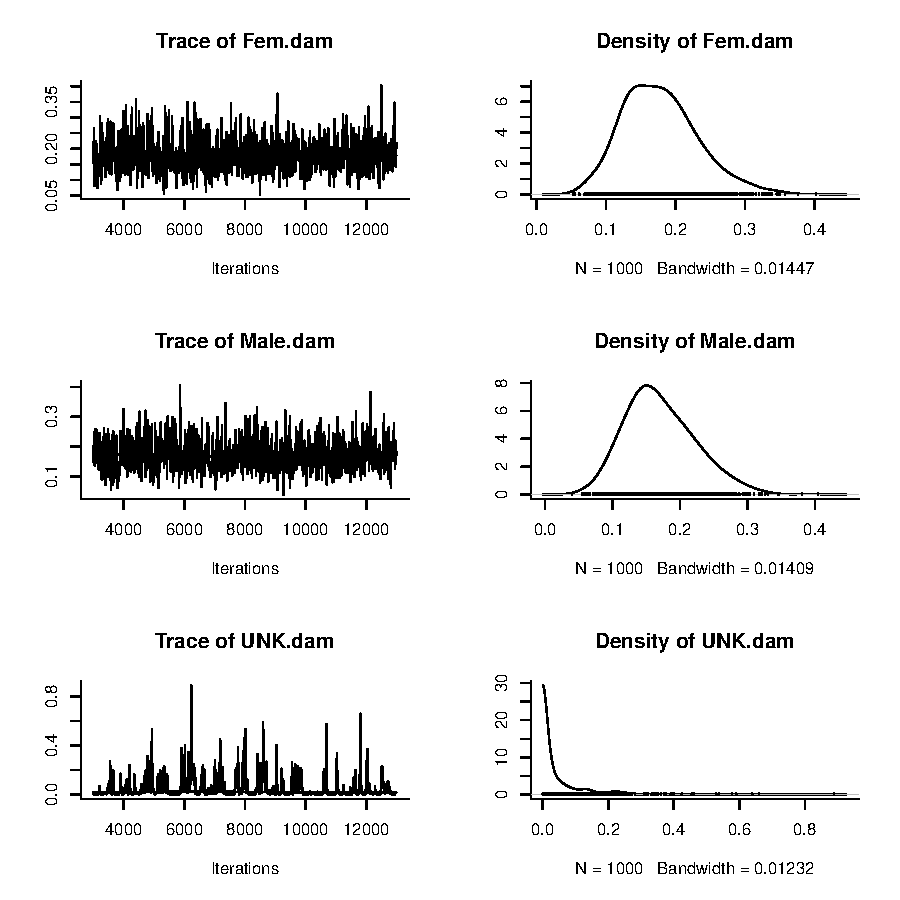
\includegraphics{Lecture3-018}
\end{center}
\caption{MCMC summary plot for the sex-specific dam variance components from model \texttt{m3a.3}. The number of chicks with unknown (\texttt{UNK}) sex is low, with very little replication within dams. The posterior distribution for the \texttt{UNK} variance component is dominated by the prior which has a marginal distribution of \texttt{V=1} and \texttt{nu=0.002}.}
\label{BTidh-fig}
\end{figure}

The sex specific variances for males and females look pretty similar, but the sex-specific variance for birds with unknown sex is not behaving well. This is not that surprising given that there are only 47 birds with unknown sex and these tend to be thinly spread across dams. This variance component is likely to be dominated by the prior, but for now we'll leave the model as it is and come back to some possible alternative solutions later.\\

We can extract the marginal means for each variance and place them into a matrix:

\begin{Schunk}
\begin{Sinput}
> Vdam.3 <- diag(colMeans(m3a.3$VCV)[1:3])
> colnames(Vdam.3) <- colnames(m3a.3$VCV)[1:3]
> Vdam.3
\end{Sinput}
\begin{Soutput}
     sexFem.dam sexMale.dam sexUNK.dam
[1,]  0.1757593   0.0000000 0.00000000
[2,]  0.0000000   0.1717858 0.00000000
[3,]  0.0000000   0.0000000 0.06184668
\end{Soutput}
\end{Schunk}

Note, that they are in general less than the marginal mean of the dam variance in model \texttt{m3a.1} (0.224)  where a sex interaction was not fitted.  Because the dam effects are assumed to be multivariate normal we can plot an ellipsoid that completely represents their distribution (you can rotate the figure in R):

\begin{Schunk}
\begin{Sinput}
> plotsubspace(Vdam.3, axes.lab = TRUE)
\end{Sinput}
\end{Schunk}

If we had measured the offspring of a lot of dams, and for each dam we had measured a very large number of offspring of each sex, then we could calculate the average tarsus lengths within a nest for males, females and unknowns separately. If we produced a scatter plot of these means the data would have the same shape as this ellipsoid and 95\% of the data would lie inside.

\begin{figure}[!h]
\begin{center}
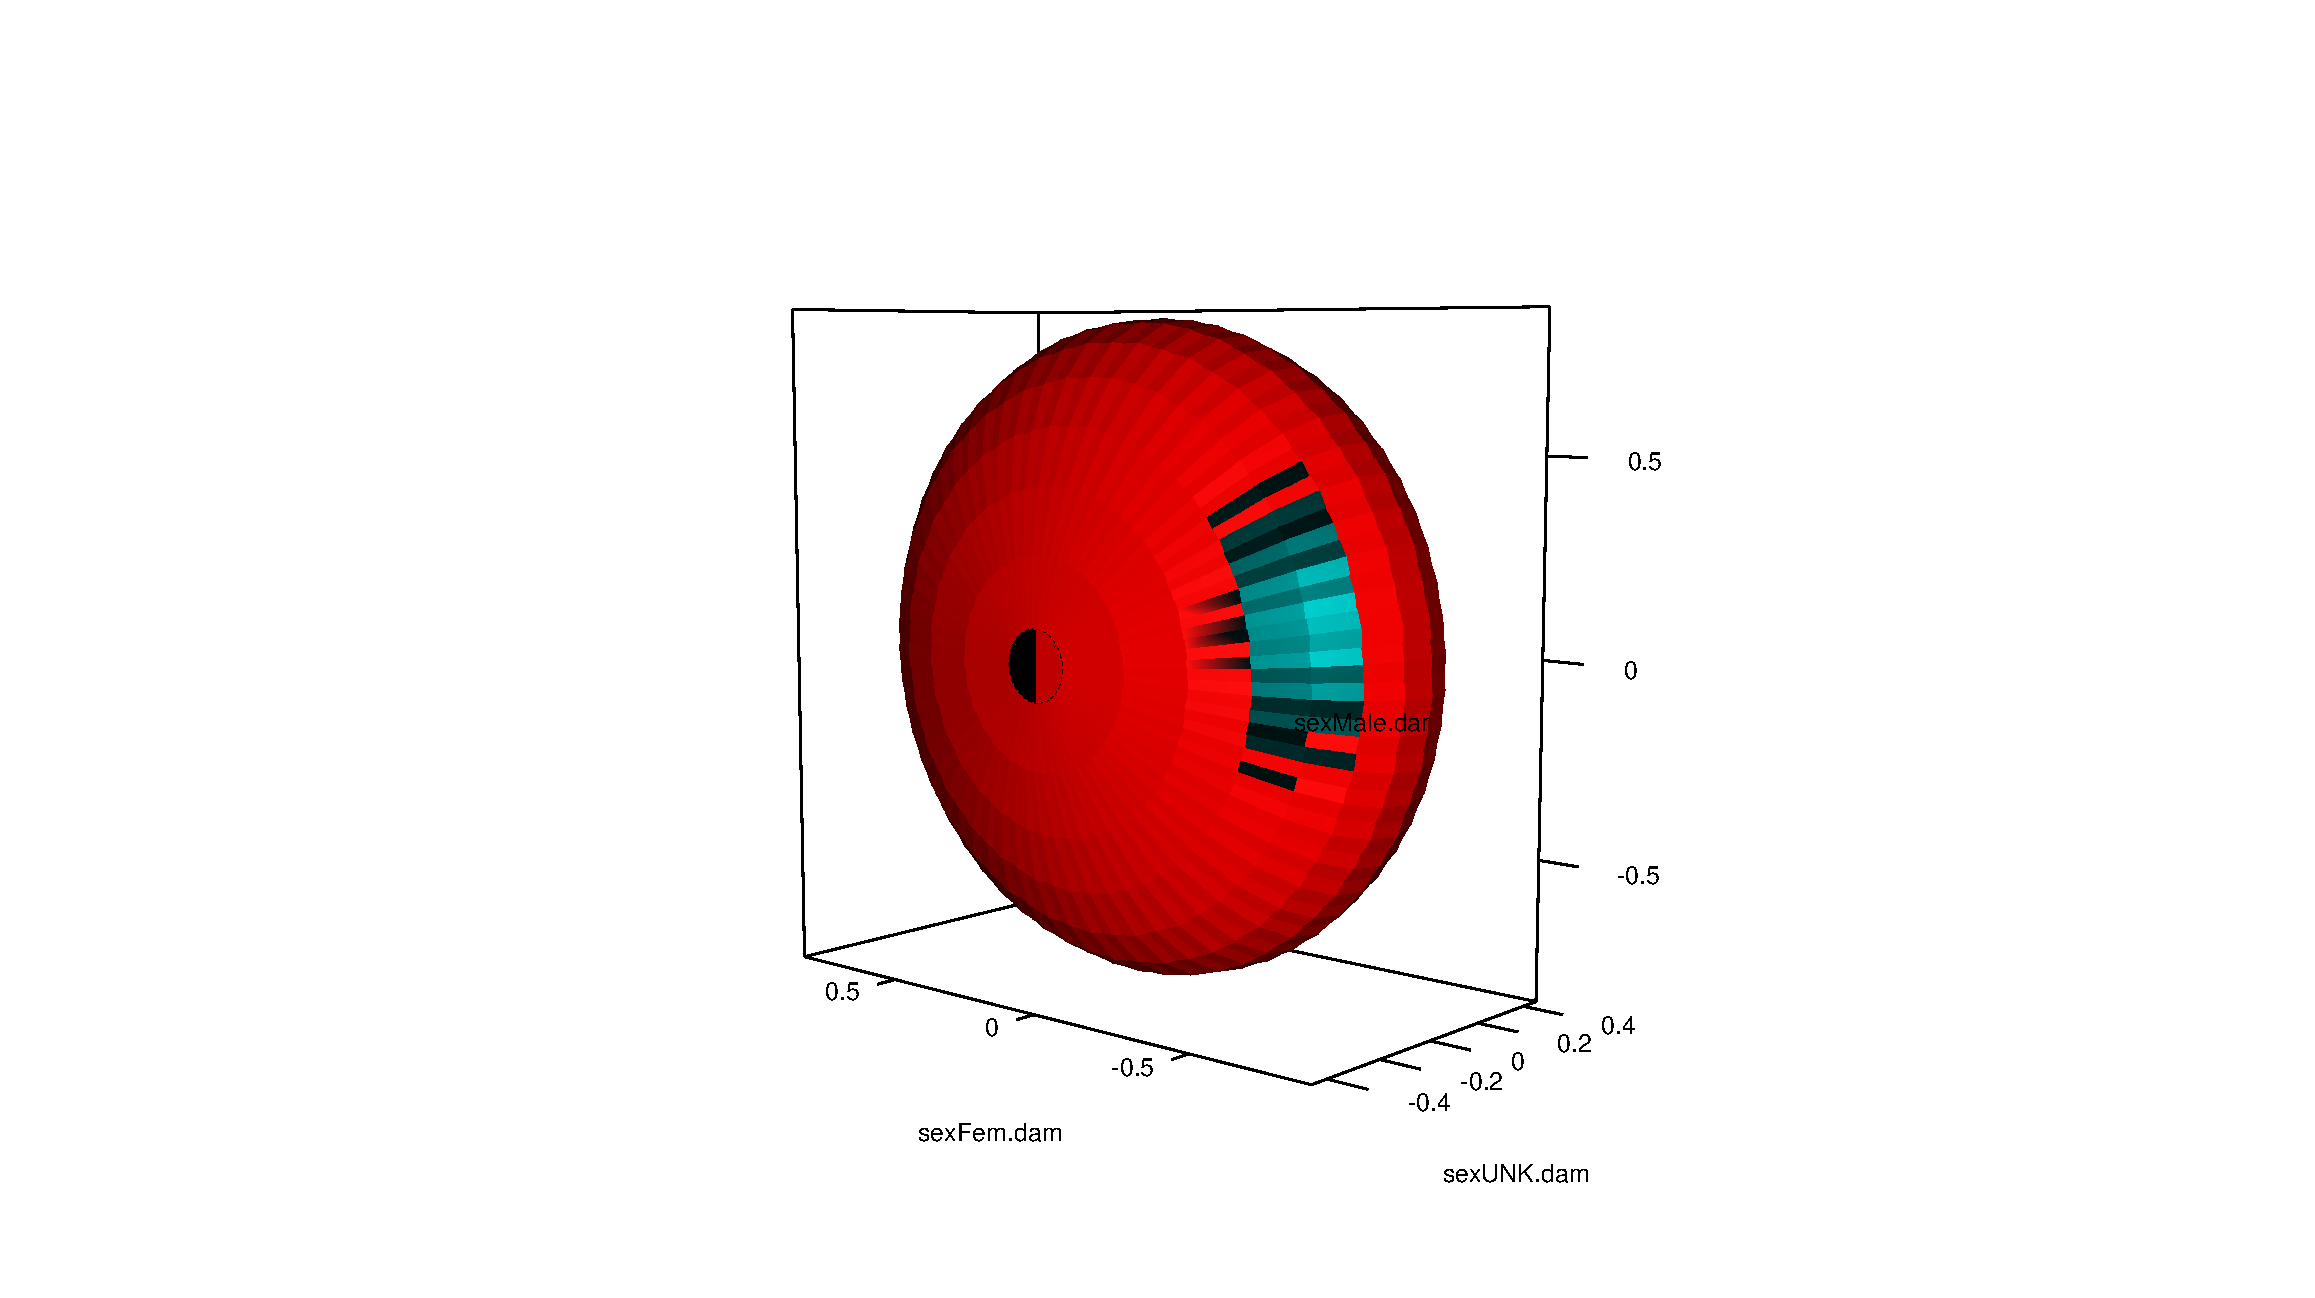
\includegraphics{rgl1.pdf}
\end{center}
\caption{Ellipsoid that circumscribes 95\% of the expected dam effects as estimated in model \texttt{m3a.3}. This can be thought of as a scatter plot of the dam effects between each sex, if the dam effects could be directly measured.  Because the covariances of the dam effects between the sexes were set to zero the axes of the ellipsoids are all parallel to the figure axes.}
\label{rgl1-fig}
\end{figure}

\section{\texttt{us} Variance Structure}

The oddity of the model, and the meaning of the off-diagonal zeros, should become apparent. We have assumed that the different sexes with in a nest are independent. If we plotted the average tarsus lengths for males against the average tarsus lengths for females for each dam this model implies we should see no relationship. We can relax this assumption using the \texttt{us} function which estimates the matrix: 

\begin{displaymath}
{\bf V}_{{\color{red} \texttt{dam}}}=
\left[
\begin{array}{ccc}
\sigma^{2}_{\color{blue}\texttt{Female}}&\sigma_{\color{blue}\texttt{Female}, \texttt{Male}}&\sigma_{\color{blue}\texttt{Female}, \texttt{UNK}}\\
\sigma_{\color{blue}\texttt{Female}, \texttt{Male}}&\sigma^{2}_{\color{blue}\texttt{Male}}&\sigma_{\color{blue}\texttt{Male}, \texttt{UNK}}\\
\sigma_{\color{blue}\texttt{Female}, \texttt{UNK}}&\sigma_{\color{blue}\texttt{Male}, \texttt{UNK}}&\sigma^{2}_{\color{blue}\texttt{UNK}}\\
\end{array}
\right]
\end{displaymath}

We will now use a prior for the covariance matrix where nu=4 (1 more than the dimension of {\bf V}) and the prior covariance matrix is an diagonal matrix with small variances. This may seem surprising but the motivation is laid out in Section \ref{VCVprior-sec}: 

\begin{Schunk}
\begin{Sinput}
> prior.m3a.4 = list(R = list(V = diag(1), nu = 0.002), 
+     G = list(G1 = list(V = diag(3) * 0.02, nu = 4), 
+         G2 = list(V = 1, nu = 0.002)))
> m3a.4 <- MCMCglmm(tarsus ~ sex, random = ~us(sex):dam + 
+     fosternest, data = BTdata, verbose = FALSE, 
+     prior = prior.m3a.4)
\end{Sinput}
\end{Schunk}

The posterior mean (co)variances for this model show that the covariances are almost the same magnitude as the variances suggesting strong correlations: 

\begin{Schunk}
\begin{Sinput}
> Vdam.4 <- matrix(colMeans(m3a.4$VCV)[1:9], 3, 
+     3)
> colnames(Vdam.4) <- colnames(m3a.4$VCV)[1:3]
> Vdam.4
\end{Sinput}
\begin{Soutput}
     sexFem:sexFem.dam sexMale:sexFem.dam sexUNK:sexFem.dam
[1,]         0.2311007          0.2004611         0.2039762
[2,]         0.2004611          0.2135747         0.1964712
[3,]         0.2039762          0.1964712         0.2424483
\end{Soutput}
\end{Schunk}

The distribution of dam effects in this model looks substantially different (Figure \ref{rgl2-fig}):

\begin{Schunk}
\begin{Sinput}
> plotsubspace(Vdam.4, axes.lab = TRUE, wire.frame = T)
\end{Sinput}
\end{Schunk}

\begin{figure}[!h]
\begin{center}
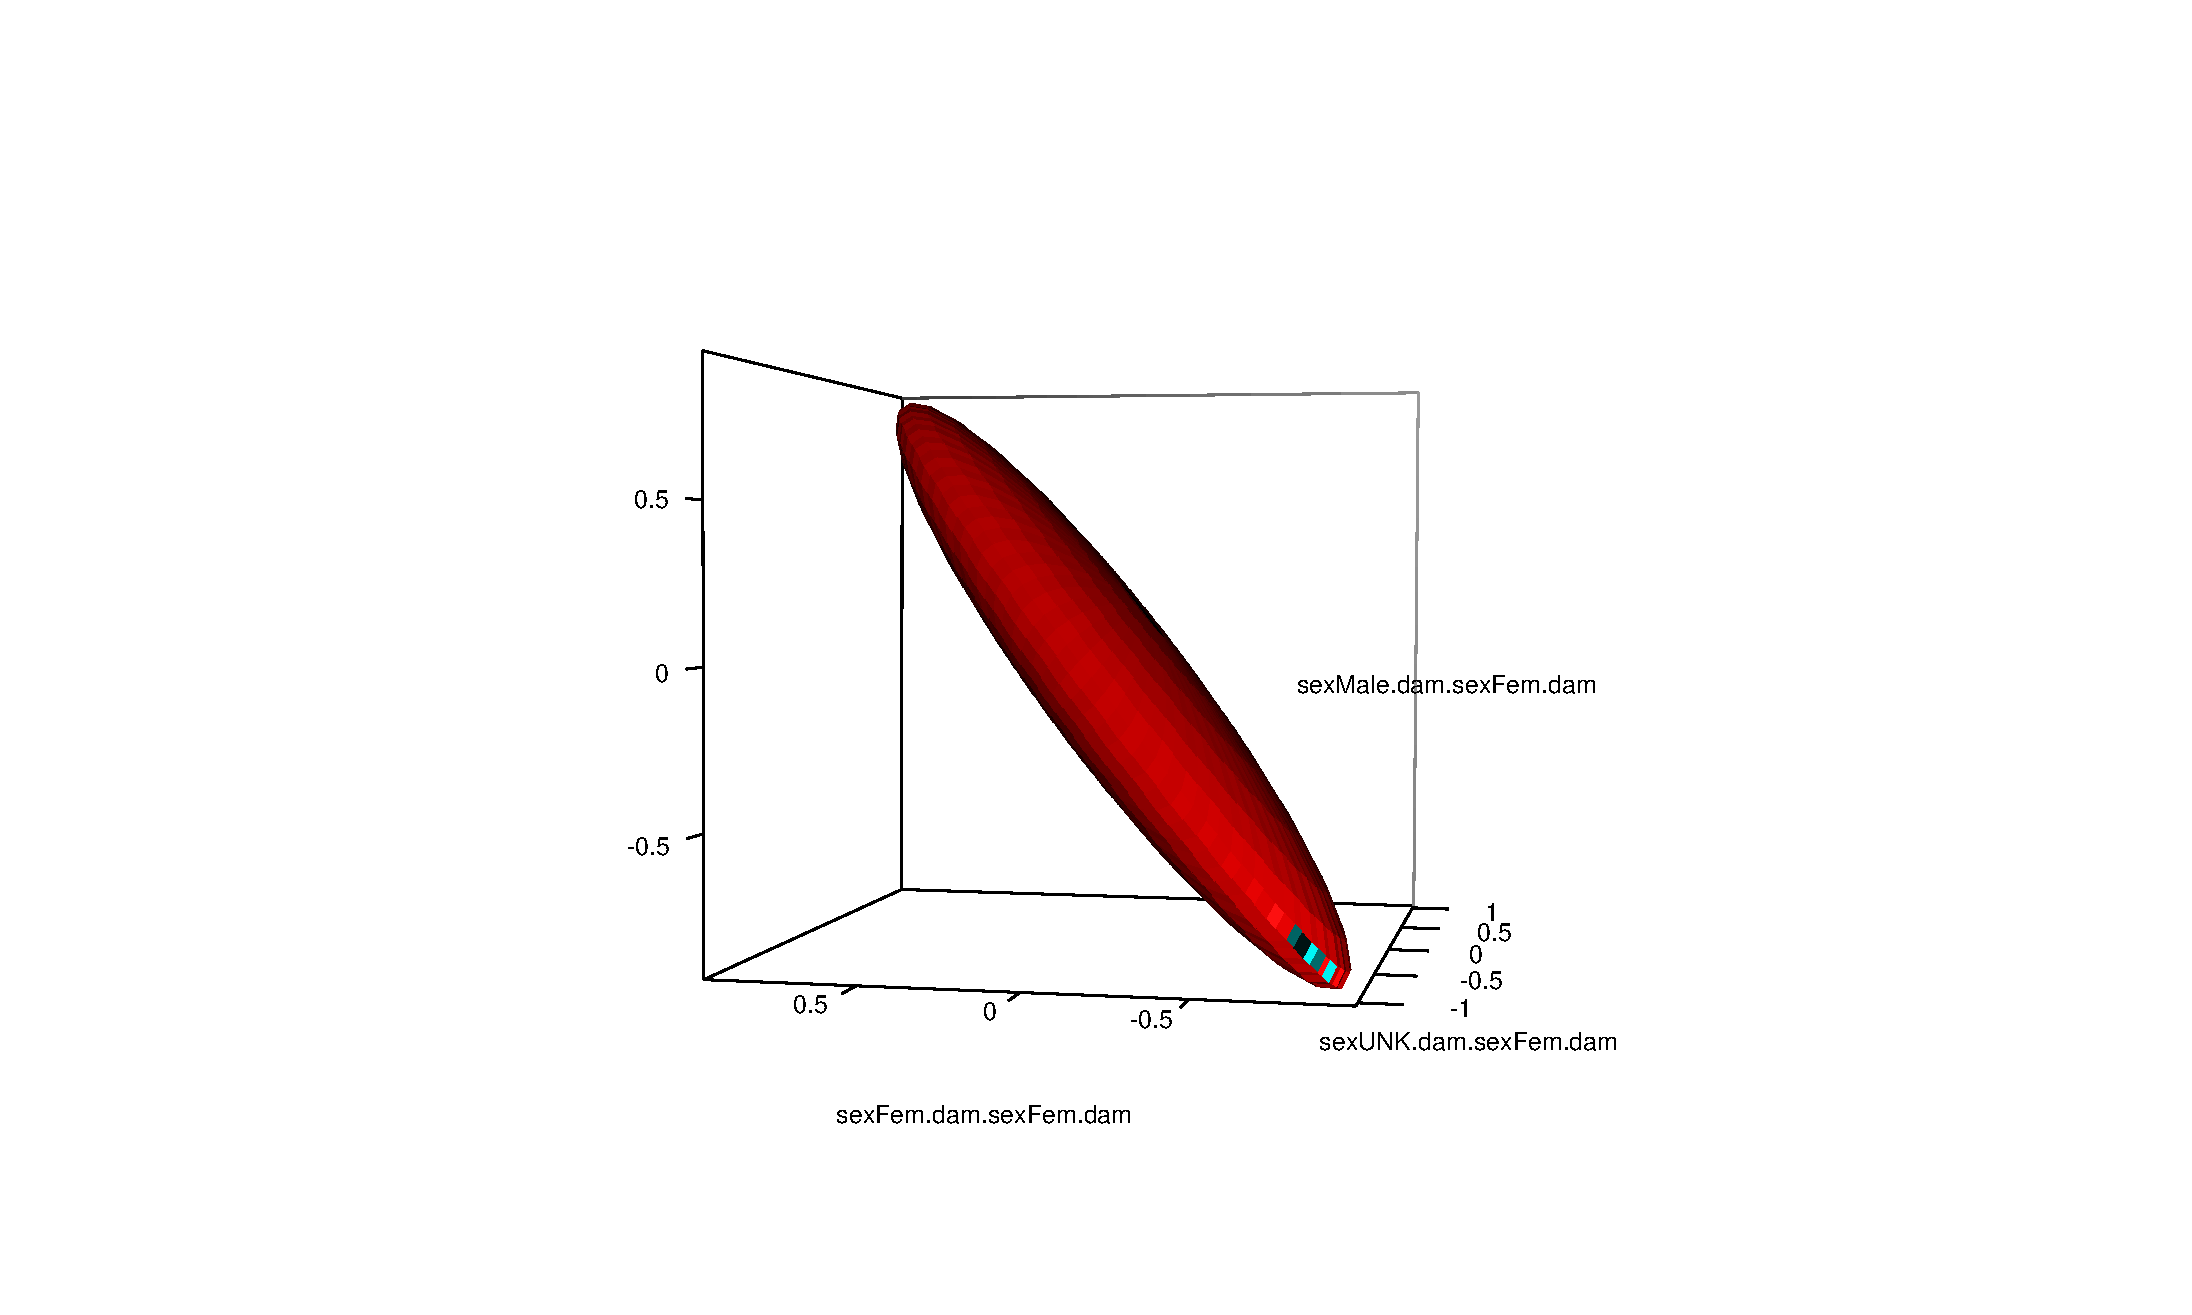
\includegraphics{rgl2.pdf}
\end{center}
\caption{Ellipsoid that circumscribes 95\% of the expected dam effects as estimated in model \texttt{m3a.4}. This can be thought of as a scatter plot of the dam effects between each sex, if the dam effects could be directly measured.  The correlations of the dam effects between the sexes were estimated and found to be close to one, and the sex-specific variances were all roughly equal in magnitude.  Consequently the major axis of the ellipsoid lies at $45^{o}$ to the figure axes.}
\label{rgl2-fig}
\end{figure}


Covariances can be hard to interpret, and I usually find correlations easier to think about. They can also be useful for detecting problems in the chain. In model \texttt{m3a.1} the dam variance for chicks with unknown sex was behaving badly and was getting `trapped' at zero. When fitting a $2\times2$ covariance matrix similar things can happen when correlations are close to -1 and 1, and this may not be obvious from the marginal distribution of the covariances:

\begin{Schunk}
\begin{Sinput}
> plot(posterior.cor(m3a.4$VCV[, 1:9])[, c(2, 3, 
+     7)])
\end{Sinput}
\end{Schunk}

\begin{figure}[!h]
\begin{center}
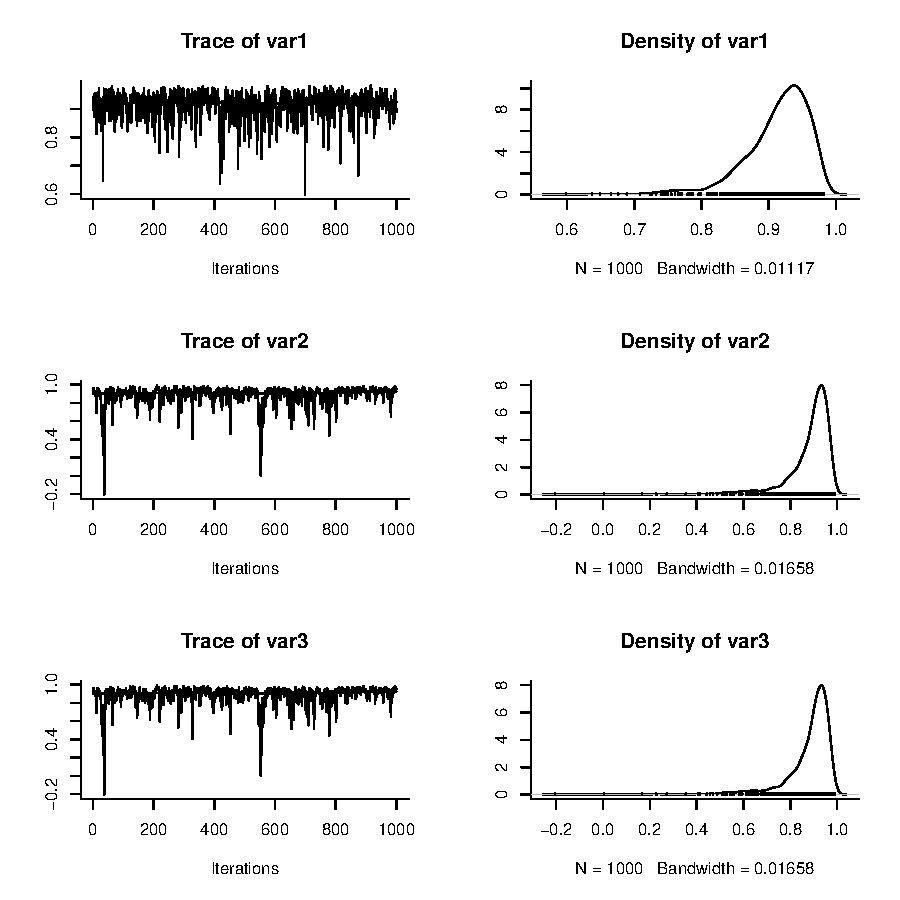
\includegraphics{Lecture3-025}
\end{center}
\caption{MCMC summary plot for the between sex correlations in dam effects from model \texttt{m3a.4}.}
\label{BTcor-fig}
\end{figure}

All the correlations are very close to one, and the variances all pretty equal so we'd probably consider the simpler model. We could try using DIC to compare models, although given the different prior specifications for the two models it is unclear whether this would be meaningful. However, the simpler model does seem to have better support as intuition suggests:

\begin{Schunk}
\begin{Sinput}
> m3a.4$DIC
\end{Sinput}
\begin{Soutput}
[1] 1997.34
\end{Soutput}
\begin{Sinput}
> m3a.1$DIC
\end{Sinput}
\begin{Soutput}
[1] 1991.29
\end{Soutput}
\end{Schunk}

\section{Compound Variance Structures}

There are also ways of specifying models that lie somewhere between the simple model (\texttt{mBT}), where dam effects are assumed to be equivalent across the sexes, and the most complex model (\texttt{mBT2}), where dam effects are allowed to vary across the sexes and covary between the sexes to different degrees. Some alternatives are listed in Table \ref{rspec}.\\

To be completed ....\\

\pagestyle{empty}
\begin{landscape}
%\footnotesize
%\begin{center}
%\begin{longtable}{ccccc}
\begin{table}
\begin{tabular}{ccccc}
\hline
\texttt{lmer} & \texttt{MCMCglmm}/\texttt{asreml}&No. Parameters&Variance&Correlation\\
\hline
\\
\texttt{(1|dam)}&\texttt{dam}&1&
$\left[
\begin{array}{ccc}
V&V&V\\
V&V&V\\
V&V&V\\
\end{array}
\right]$
&
$\left[
\begin{array}{ccc}
{\color{red} 1}&{\color{red} 1}&{\color{red} 1}\\
{\color{red} 1}&{\color{red} 1}&{\color{red} 1}\\
{\color{red} 1}&{\color{red} 1}&{\color{red} 1}\\
\end{array}
\right]$\\
\\
\texttt{(sex-1|dam)}&\texttt{us(sex):dam}&6&
$\left[
\begin{array}{ccc}
V_{1,1}&C_{1,2}&C_{1,3}\\
C_{1,2}&V_{2,2}&C_{2,3}\\
C_{1,3}&C_{2,3}&V_{3,3}\\
\end{array}
\right]$
&
$\left[
\begin{array}{ccc}
{\color{red} 1}&r_{1,2}&r_{1,3}\\
r_{1,2}&{\color{red} 1}&r_{2,3}\\
r_{1,3}&r_{2,3}&{\color{red} 1}\\
\end{array}
\right]$\\
\\
\texttt{(1|sex:dam)}&\texttt{sex:dam}&1&
$\left[
\begin{array}{ccc}
V&{\color{red} 0}&{\color{red} 0}\\
{\color{red} 0}&V&{\color{red} 0}\\
{\color{red} 0}&{\color{red} 0}&V\\
\end{array}
\right]$
&
$\left[
\begin{array}{ccc}
{\color{red} 1}&{\color{red} 0}&{\color{red} 0}\\
{\color{red} 0}&{\color{red} 1}&{\color{red} 0}\\
{\color{red} 0}&{\color{red} 0}&{\color{red} 1}\\
\end{array}
\right]$\\
\\
\texttt{(1|dam)}+\texttt{(1|sex:dam)}&\texttt{dam}+\texttt{sex:dam}&2&
$\left[
\begin{array}{ccc}
V_{1}+V_{2}&V_{1}&V_{1}\\
V_{1}&V_{1}+V_{2}&V_{1}\\
V_{1}&V_{1}&V_{1}+V_{2}\\
\end{array}
\right]$
&
$\left[
\begin{array}{ccc}
{\color{red} 1}&r&r\\
r&{\color{red} 1}&r\\
r&r&{\color{red} 1}\\
\end{array}
\right]$\\
\\
-&\texttt{idh(sex):dam}&3&
$\left[
\begin{array}{ccc}
V_{1,1}&{\color{red} 0}&{\color{red} 0}\\
{\color{red} 0}&V_{2,2}&{\color{red} 0}\\
{\color{red} 0}&{\color{red} 0}&V_{3,3}\\
\end{array}
\right]$
&
$\left[
\begin{array}{ccc}
{\color{red} 1}&{\color{red} 0}&{\color{red} 0}\\
{\color{red} 0}&{\color{red} 1}&{\color{red} 0}\\
{\color{red} 0}&{\color{red} 0}&{\color{red} 1}\\
\end{array}
\right]$\\
%-&\texttt{idh(1+sex):dam}&3&
%$\left[
%\begin{array}{ccc}
%V_{1,1}&V_{1,1}&V_{1,1}\\
%V_{1,1}&V_{1,1}+V_{2,2}&V_{1,1}\\
%V_{1,1}&V_{1,1}&V_{1,1}+V_{3,3}\\
%\end{array}
%\right]$
%&
%$\left[
%\begin{array}{ccc}
%V_{1,1}&\frac{V_{1,1}}{\sqrt{V_{1,1}(V_{1,1}+V_{2,2})}}&\frac{V_{1,1}}{\sqrt{V_{1,1}(V_{1,1}+V_{3,3})}}\\
%\frac{V_{1,1}}{\sqrt{V_{1,1}(V_{1,1}+V_{2,2})}}&V_{1,1}+V_{2,2}&\frac{V_{1,1}}{\sqrt{(V_{1,1}+V_{2,2})(V_{1,1}+V_{3,3})}}\\
%\frac{V_{1,1}}{\sqrt{V_{1,1}(V_{1,1}+V_{3,3})}}&\frac{V_{1,1}}{\sqrt{(V_{1,1}+V_{2,2})(V_{1,1}+V_{3,3})}}&V_{1,1}+V_{3,3}\\
%\end{array}
%\right]$\\
%-&\texttt{us(at.level(sex, 2)+set.level(sex, c(1, 3)):dam}&$\left[
%\begin{array}{ccc}
%V_{1,1}&C_{1,2}&C_{1,3}\\
%C_{1,2}&V_{2,2}&C_{2,3}\\
%C_{1,3}&C_{2,3}&V_{3,3}\\
%\end{array}
%\right]$
%&
%$\left[
%\begin{array}{ccc}
%1&r_{1,2}&r_{1,3}\\
%r_{1,2}&1&r_{2,3}\\
%r_{1,3}&r_{2,3}&1\\
%\end{array}
%\right]$\\
%\\
%-&\texttt{corh(sex):dam}&4&
%$\left[
%\begin{array}{ccc}
%V_{1,1}&r\sqrt{V_{1,1}V_{2,2}}&r\sqrt{V_{1,1}V_{2,2}}\\
%r\sqrt{V_{1,1}V_{2,2}}&V_{2,2}&r\sqrt{V_{2,2}V_{2,3}}\\
%r\sqrt{V_{1,1}V_{3,3}}&r\sqrt{V_{2,2}V_{3,3}}&V_{3,3}\\
%\end{array}
%\right]$
%&
%$\left[
%\begin{array}{ccc}
%{\color{red} 1}&r&r\\
%r&{\color{red} 1}&r\\
%r&r&{\color{red} 1}\\
%\end{array}
%\right]$\\
\\
-&\texttt{corg(sex):dam}&3&
$\left[
\begin{array}{ccc}
{\color{red} 1}&r_{1,2}&r_{1,3}\\
r_{1,2}&{\color{red} 1}&r_{2,3}\\
r_{1,3}&r_{2,3}&{\color{red} 1}\\
\end{array}
\right]$
&
$\left[
\begin{array}{ccc}
{\color{red} 1}&r_{1,2}&r_{1,3}\\
r_{1,2}&{\color{red} 1}&r_{2,3}\\
r_{1,3}&r_{2,3}&{\color{red} 1}\\
\end{array}
\right]$\\
\\
-&\texttt{corgh(sex):dam}&3&
$\left[
\begin{array}{ccc}
{\color{red} V_{1,1}}&r_{1,2}\sqrt{{\color{red} V_{1,1}V_{2,2}}}&r_{1,3}\sqrt{{\color{red} V_{1,1}V_{2,2}}}\\
r_{1,2}\sqrt{{\color{red} V_{1,1}V_{2,2}}}&{\color{red} V_{2,2}}&r_{2,3}\sqrt{{\color{red} V_{2,2}V_{2,3}}}\\
r_{1,3}\sqrt{{\color{red} V_{1,1}V_{3,3}}}&r_{2,3}\sqrt{{\color{red} V_{2,2}V_{3,3}}}&{\color{red} V_{3,3}}\\
\end{array}
\right]$
&
$\left[
\begin{array}{ccc}
{\color{red} 1}&r_{1,2}&r_{1,3}\\
r_{1,2}&{\color{red} 1}&r_{2,3}\\
r_{1,3}&r_{2,3}&{\color{red} 1}\\
\end{array}
\right]$\\
\\
\hline
\end{tabular}
\caption{Different random effect specifications in \texttt{lmer}, \texttt{MCMCglmm} and \texttt{asreml}. \texttt{sex} is a factor with three levels so the resulting matrix is $3\times3$. Continuous variables can also go on the LHS of the pipe, or within the variance structure functions (e.g. \texttt{us},\texttt{idh}). In this case the associated parameters are regression coefficients for which a variance is estimated. For example, if the chicks were of different ages (or we'd measured the same chicks at different ages) we may want to see if the growth rate is more similar for chicks raised by the same mother. \texttt{(1+age|dam)} or \texttt{us(1+age):dam} estimates a $2\times2$ matrix which includes the variance in intercepts (when \texttt{age}=0), the variance in slopes, and the covariance that exists between them. Fixed parameters are in red.}
\label{rspec}
\end{table}
%\end{longtable}
%\end{center}
\end{landscape}
\pagestyle{headings}

\section{Heterogenous Residual Variance}
\label{heter-sec}
To be started... In short - if you've fitted a sex by dam interaction I would always allow the sexes to have different residual variances. Use \texttt{rcov=$\sim$idh(sex):units}.

\section{Contrasts and Covariances}

A general method for seeing what a particular random specification means in terms of the original variables is to realise that 

\begin{equation}
{\bm \Sigma} = {\bf Z}{\bf V}{\bf Z}^{'}
\label{conv-eq}
\end{equation}

where ${\bm \Sigma}$ is the covariance matrix for the original set of variables and ${\bf V}$ the variances associated with the variance structure model. ${\bf Z}$ is the random effect design matrix. Equation \ref{conv-eq} implies:

\begin{equation}
{\bf V} = {\bf Z}^{-1}{\bm \Sigma}({\bf Z}^{'})^{-1}
\end{equation}

or alternatively: 

\begin{equation}
{\bf V} = ({\bf Z}{\bf Z}^{'})^{-}{\bf Z}^{'}{\bm \Sigma}{\bf Z}({\bf Z}^{'}{\bf Z})^{-}
\end{equation}

if ${\bf Z}$ is non-square and/or singular, where \texttt{$^{-}$} is a generalised inverse.\\

 
\section{Priors for Covariance Matrices}
\label{VCVprior-sec}

Priors for covariance matrices are tricky. What maybe non-informative for a covariance may be informative for a correlation and \emph{vice versa}.

\subsection{Priors for \texttt{us} structures}

A useful result is that the marginal distribution of a variance is also inverse - Wishart distributed:

\begin{displaymath}
\sigma^{2}_{1} \sim IW\left(\texttt{nu}^{\ast}\texttt{=nu-dim(V)+1},\ \texttt{V}^{\ast}=\frac{\texttt{nu}}{\texttt{nu}^{\ast}}\texttt{V[1,1]}\right)
\end{displaymath}

using the first variance as an example, and indicating the new parameters with an asterisk.\\

An uninformative prior for the correlations is an improper prior with \texttt{V=diag(dim(V))$\ast$0} and \texttt{nu=dim(V)+1}. For the $3\times3$ sex by dam covariance matrix in model \texttt{m3a.4} we used a proper prior with \texttt{V=diag(3)$\ast$0.02} and \texttt{nu=4} in the hope that this would be relatively uninformative for the correlations. We can plot the marginal density of the variances for this distribution as we did in Chapter \ref{chap1}:

\begin{Schunk}
\begin{Sinput}
> nu.ast <- prior.m3a.4$G$G1$nu - dim(prior.m3a.4$G$G1$V)[1] + 
+     1
> V.ast <- prior.m3a.4$G$G1$V[1, 1] * (prior.m3a.4$G$G1$nu/nu.ast)
> xv <- seq(1e-16, 1, length = 100)
> dv <- MCMCpack::dinvgamma(xv, shape = nu.ast/2, 
+     scale = (nu.ast * V.ast)/2)
> plot(dv ~ xv, type = "l")
\end{Sinput}
\end{Schunk}

\begin{figure}[!h]
\begin{center}
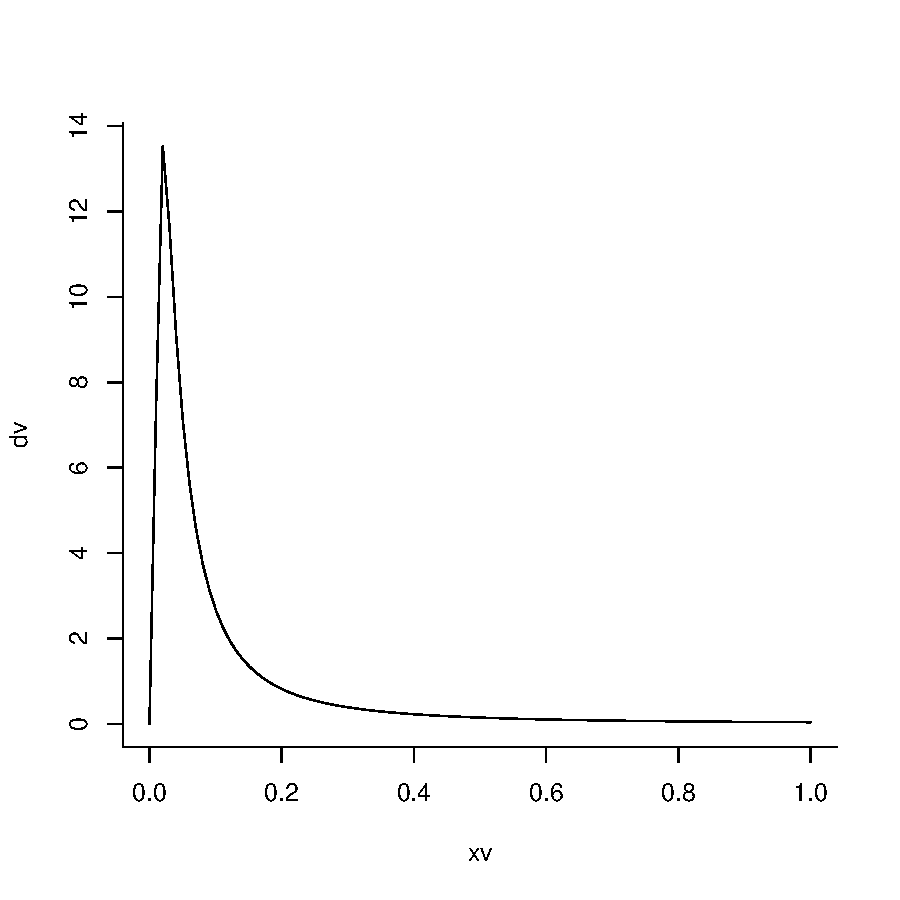
\includegraphics{Lecture3-028}
\end{center}
\caption{Marginal prior distribution of a variance using an inverse Wishart prior for the covariance matrix with \texttt{V=diag(3)*0.02} and \texttt{nu=4}.}
\label{NIc-fig}
\end{figure}


In Chapter \ref{chap2} we saw that a non-informative prior for a variance component was \texttt{V=0} and \texttt{nu=-2}. This result generalises to covariance matrices where the improper prior \texttt{V=diag(dim(V))$\ast$0} and \texttt{nu=dim(V)-3} is non-informative for the variances and covariances. This can be verified for the variances using the results derived above for the marginal distribution:

\begin{displaymath}
\begin{array}{rl}
\sigma^{2}_{1} \sim& IW\left(\texttt{nu}^{\ast}\texttt{=dim(V)-3-dim(V)+1},\ \texttt{V}^{\ast}=\frac{\texttt{nu}}{\texttt{nu}^{\ast}}\texttt{0}\right)\\
               \sim& IW\left(\texttt{nu}^{\ast}\texttt{=-2},\ \texttt{V}^{\ast}=\texttt{0}\right)\\

\end{array}
\end{displaymath}

\subsection{Priors for \texttt{idh} structures}

For \texttt{idh} the diagonal elements of the matrix are independent and each variance is distributed as\footnote{IMPORTANT: In versions $<$ 2.05 priors on each variance of an \texttt{idh} structure were distributed as $IW\left(\texttt{nu}^{\ast}\texttt{=nu-dim(V)+1},\ \texttt{V}^{\ast}=\texttt{V[1,1]}\right)$ but this was a source of confusion and was changed.}:

\begin{displaymath}
\sigma^{2}_{1} \sim IW\left(\texttt{nu}^{\ast}\texttt{=nu},\ \texttt{V}^{\ast}=\texttt{V[1,1]}\right)
\end{displaymath}


\subsection{Priors for \texttt{corg} and \texttt{corgh} structures}

For \texttt{corg} and \texttt{corgh} structures\footnote{In versions $<2.18$ \texttt{cor} fitted what is now a \texttt{corg} structure. The reason for the change is to keep the \texttt{asreml} and  \texttt{MCMCglmm} syntax equivalent. However, the \texttt{corgh} structure in asreml is a reparameterised \texttt{us} structure whereas in \texttt{MCMCglmm} the variances are fixed in the prior.} the diagonals of \texttt{V} define the fixed variances (\texttt{corgh}) or are ignored and the variances set to one (\texttt{corg}). I use the prior specification in \citet{Barnard.2000} where \texttt{nu} controls how much the correlation matrix approaches an identity matrix.  The marginal distribution of individual correlations ($r$) is given by \citet{Barnard.2000}   \citep[and][]{Box.1973}:

\begin{equation}
\begin{array}{lr}
Pr(r) \propto (1-r^{2})^\frac{\texttt{nu-dim(V)-1}}{\texttt{2}}, & |r|<1\\
\end{array}
\end{equation}

and as shown above setting \texttt{nu} =\texttt{dim(V)+1} results in marginal correlations that are uniform on the interval [-1,1].\\

In most cases correlation matrices do not have known form and so cannot be directly Gibbs sampled. \texttt{MCMCglmm} uses a method proposed by \citet{Liu.2006} with the target prior as in \citet{Barnard.2000}.  Generally this algorithm is very efficient as the Metropolis-Hastings acceptance probability only depends on the degree to which the candidate prior  and the target prior (the prior you specify) conflict. The candidate prior is equivalent to the prior  in \citet{Barnard.2000} with \texttt{nu=0} so as long as a diffuse prior is set, mixing is generally not a problem. If  \texttt{nu=0} is set (the default) then the Metropolis-Hastings steps are always accepted resulting in Gibbs sampling. However, a prior of this form puts high density on extreme correlations which can cause problems if the data give support to correlations in this region.\\ 

\label{VCVprior-sec}
\ifalone
\end{document}
\else
\fi


\newif\ifalone
\alonefalse
\newif\iftalk
\talktrue

\ifalone
\documentclass{article}
\usepackage{graphicx}
\usepackage{natbib}
\usepackage{amsfonts}
\usepackage{amssymb}
\usepackage{amsthm}
\usepackage{bm}
\usepackage{Sweave}
\usepackage{lscape}
\usepackage{makeidx}
\usepackage{color}
\usepackage{hyperref}

\let\proglang=\textsf
\newcommand{\pkg}[1]{{\fontseries{b}\selectfont #1}}
  \hypersetup{%
    hyperindex = {true},
    colorlinks = {true},
    linktocpage = {true},
    plainpages = {false},
    linkcolor = {blue},
    citecolor = {blue},
    urlcolor = {red},
    pdfstartview = {Fit},
    pdfpagemode = {UseOutlines},
    pdfview = {XYZ null null null}
  }

\title{Continuous Random Interactions}

\author{Jarrod Hadfield (\texttt{j.hadfield@ed.ac.uk})}
\begin{document}
\maketitle
\else
\chapter{Continuous Random Interactions}
\label{chap4}
\fi


In Lecture \ref{chap3} we saw how we could define a linear model within a variance function and then interact these terms with a random effect. In the example, we did this in order to fit a \texttt{sex} by \texttt{dam} interaction:

\begin{Schunk}
\begin{Soutput}
us(sex):dam
\end{Soutput}
\end{Schunk}

The term entering into the variance function model was categorical, and we saw that by fitting the interaction we were essentially estimating the parameters of the covariance matrix:   

\begin{displaymath}
{\bf V}_{{\color{red} \texttt{dam}}}=
\left[
\begin{array}{ccc}
\sigma^{2}_{\color{blue}\texttt{Female}}&\sigma_{\color{blue}\texttt{Female}, \texttt{Male}}&\sigma_{\color{blue}\texttt{Female}, \texttt{UNK}}\\
\sigma_{\color{blue}\texttt{Female}, \texttt{Male}}&\sigma^{2}_{\color{blue}\texttt{Male}}&\sigma_{\color{blue}\texttt{Male}, \texttt{UNK}}\\
\sigma_{\color{blue}\texttt{Female}, \texttt{UNK}}&\sigma_{\color{blue}\texttt{Male}, \texttt{UNK}}&\sigma^{2}_{\color{blue}\texttt{UNK}}\\
\end{array}
\right]
\end{displaymath}

We are also free to define the variance function model with continuous covariates, or even a mixture of continuous and categorical factors, and the resulting covariance matrix is interpreted in the same way.

\section{Random Regression}

 As an example, we'll use a longitudinal data set on chicken growth (See Figure \ref{ChickWeight-fig}):

\begin{Schunk}
\begin{Sinput}
> data(ChickWeight)
\end{Sinput}
\end{Schunk}

The data consist of body weights (\texttt{weight}) for 50 chicks (\texttt{Chick}) measured up to 12 times over a 3 week period. The variable \texttt{Time} is the number of days since hatching, and \texttt{Diet} is a four level factor indicating the type of protein diet the chicks received.

\begin{Schunk}
\begin{Sinput}
> xyplot(weight ~ Time | Chick, data = ChickWeight)
\end{Sinput}
\end{Schunk}


\begin{figure}[!h]
\begin{center}
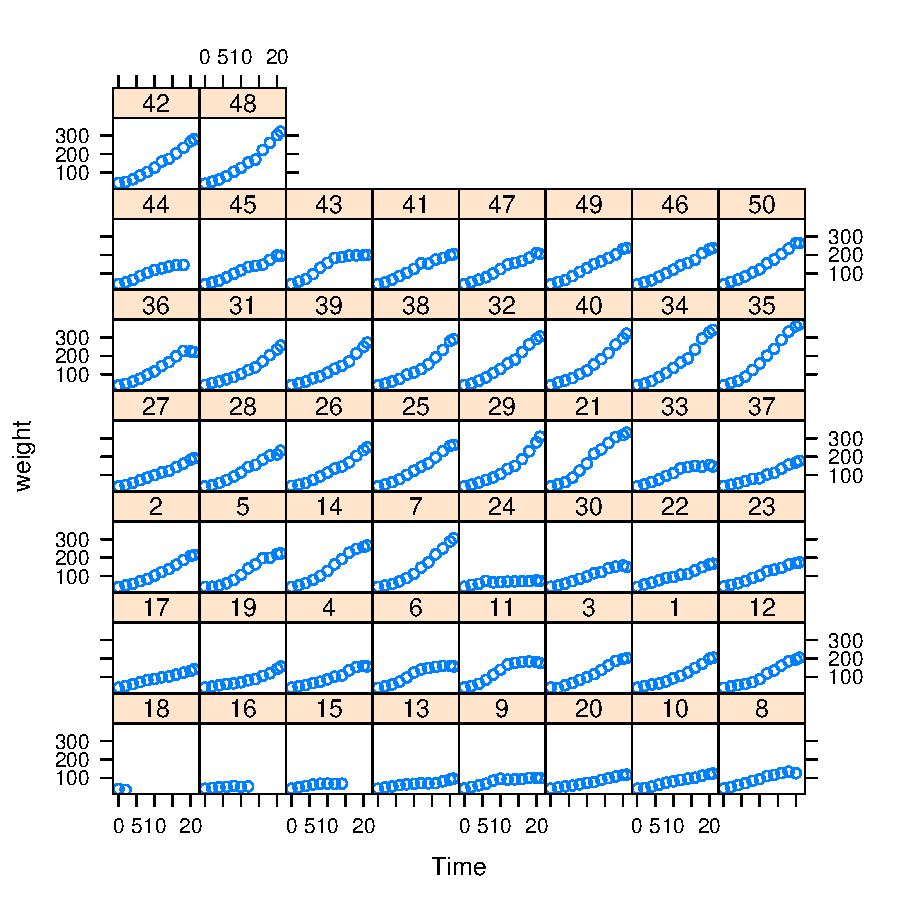
\includegraphics{Lecture4-005}
\end{center}
\caption{Weight data of 50 chicks from hatching until three weeks old.}
\label{ChickWeight-fig}
\end{figure}

Growth curves tend to be sigmoidal and so one of the non-linear growth curves such as the Gompertz or logistic may be a good starting model. However, these can be tricky to use and an alternative is to try and capture the form of the curve using polynomials. We'll start with a quadratic function at the population level and and fit chick as a random term:

\begin{Schunk}
\begin{Sinput}
> prior.m4a.1 <- list(R = list(V = 1e-16, n = -2), G = list(G1 = list(V = 1, 
+     n = 1)))
> m4a.1 <- MCMCglmm(weight ~ Diet + poly(Time, 2, raw = TRUE), 
+     random = ~Chick, data = ChickWeight, verbose = FALSE, pr = TRUE, 
+     prior = prior.m4a.1, saveX = TRUE, saveZ = TRUE)
\end{Sinput}
\end{Schunk}

We've saved the random chick effects so we can plot the predicted growth functions for each bird. For now we will just predict the growth function assuming that all birds were on Diet 1 (the intercept): 

\begin{Schunk}
\begin{Sinput}
> pop.int <- posterior.mode(m4a.1$Sol[, 1])
> pop.slope <- posterior.mode(m4a.1$Sol[, 5])
> pop.quad <- posterior.mode(m4a.1$Sol[, 6])
> chick.int <- posterior.mode(m4a.1$Sol[, c(7:56)])
\end{Sinput}
\end{Schunk}

We need to combine these parameter estimates with the polynomials for \texttt{Time} which are just the sequence $\texttt{Time}^{0}, \texttt{Time}^1, \texttt{Time}^2 \dots$ and so on. We can then plot the population expected population growth curve, and around that the predicted growth curves for each chick (we don't need to bother with $\texttt{Time}^{0}$ since this is always one):

\iftalk
\else

\begin{Schunk}
\begin{Sinput}
> pos.time <- seq(0, 21, length = 100)
> plot(pop.int + pop.slope * I(pos.time^1) + pop.quad * I(pos.time^2) ~ 
+     pos.time, type = "l", lwd = 2, ylim = c(-25, 400))
> for (i in 1:50) {
+     lines(pop.int + chick.int[i] + pop.slope * I(pos.time^1) + 
+         pop.quad * I(pos.time^2) ~ pos.time, col = "red", lty = 2)
+ }
\end{Sinput}
\end{Schunk}
\fi

\begin{figure}[!h]
\begin{center}
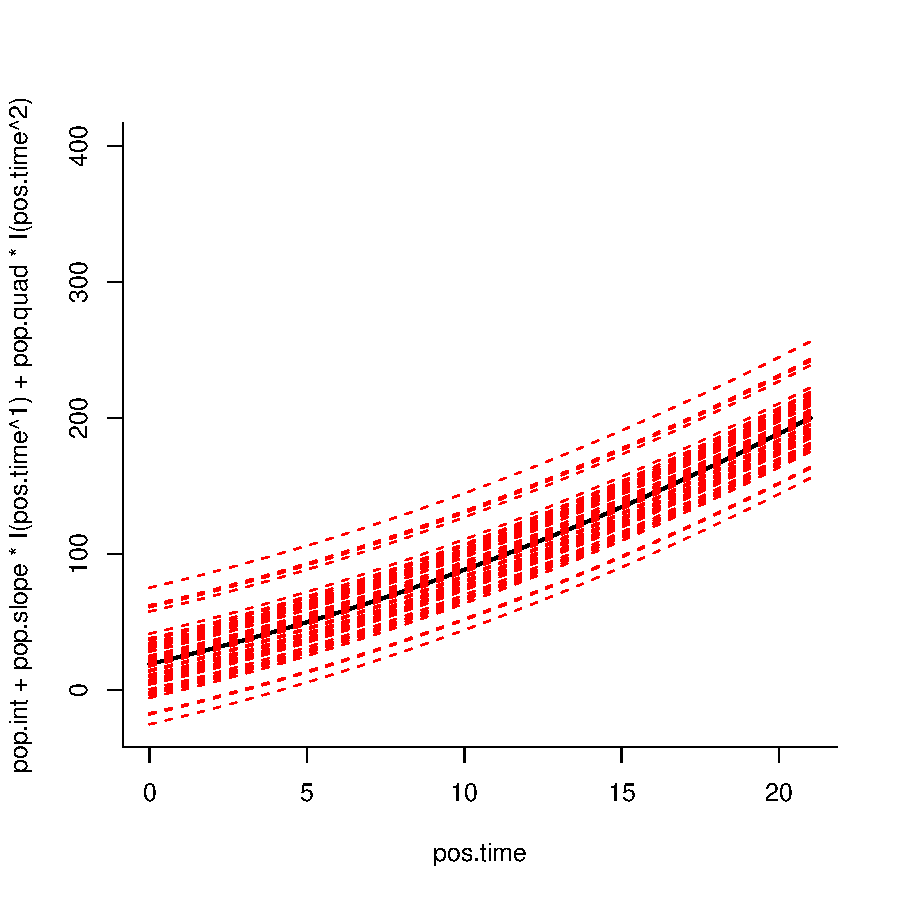
\includegraphics{Lecture4-011}
\end{center}
\caption{Predicted weights of each chick as a function of age. A quadratic population growth curve (black) is fitted with random chick intercepts.}
\label{CWpred.1-fig}
\end{figure}

The population growth curve is slightly convex because of the quadratic term, and the predictions for each chick are parallel to this curve. By fitting chick as a random effect we have allowed variation in the intercept only, and often this is not enough. We can get a feel for how well the model fits the data by overlaying the predictions with actual values. In the call to \texttt{MCMCglmm} we specified \texttt{saveX=TRUE} and \texttt{saveZ=TRUE} indicating that we wanted to save the design matrices. We can combine these matrices into the design matrix ${\bf W}$ and multiply by the parameter vector ${\bm \theta}$ to get the predictions (See Eq. \ref{MM-eq}):

\begin{Schunk}
\begin{Sinput}
> W.1<-cBind(m4a.1$X, m4a.1$Z)  # note X and Z are sparse so use cBind
> prediction.1<-W.1%*%posterior.mode(m4a.1$Sol)
> xyplot(weight+prediction.1@x~Time|Chick, data=ChickWeight)
\end{Sinput}
\end{Schunk}


\begin{figure}[!h]
\begin{center}
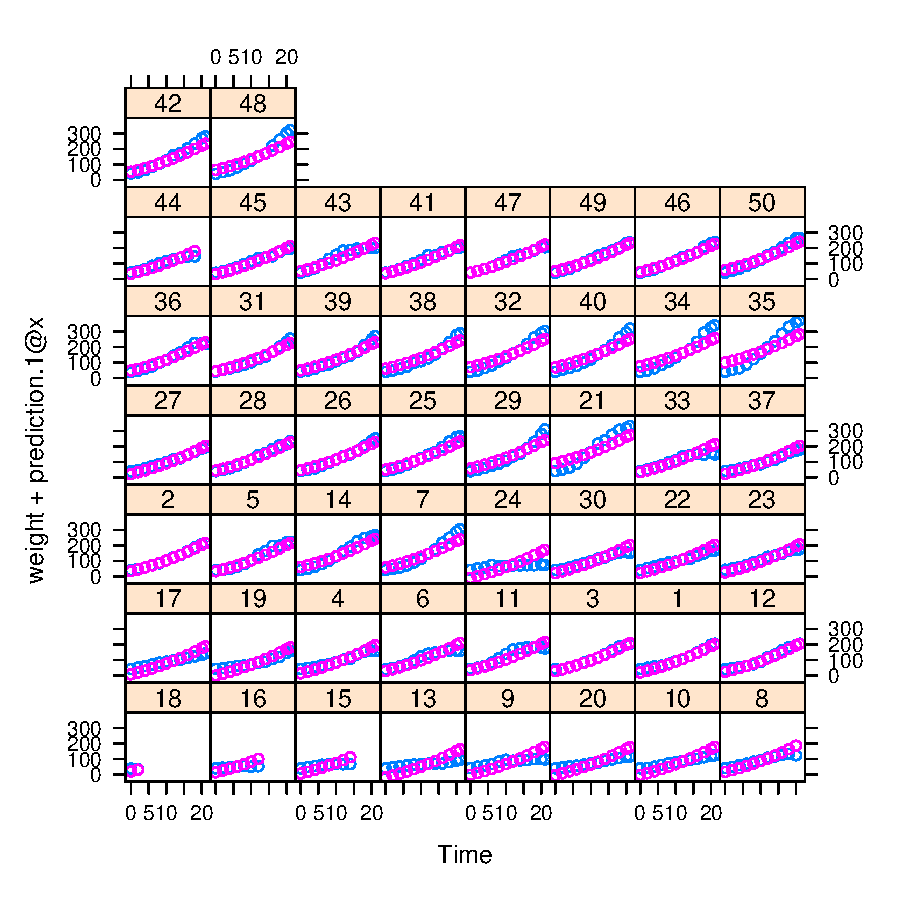
\includegraphics{Lecture4-014}
\end{center}
\caption{Weights of each chick as a function of age in blue, with the predicted weights in purple. A quadratic population growth curve was fitted with random chick intercepts.}
\label{CWpred.1-fig}
\end{figure}

The predictions don't look that bad, but you will notice that for some chicks (e.g. 13,19,34) the slope of the predicted growth seems either to shallow, or too steep. To account for this we can start by fitting \texttt{us(1+time):Chick}. The linear model inside the variance function has two parameters, an intercept (\texttt{1}) and a regression slope associated with \texttt{Time} which define the set of interactions:


\begin{displaymath}
\begin{array}{c|rrrrrc}
&{\color{red} \texttt{Chick1}}&{\color{red} \texttt{Chick2}}&{\color{red} \texttt{Chick3}}&\dots\\
\hline\\
{\color{blue} \texttt{(Intercept)}}&{\color{blue} \texttt{(Intercept)}}.{\color{red} \texttt{Chick1}}&{\color{blue} \texttt{(Intercept)}}.{\color{red} \texttt{Chick2}}&{\color{blue} \texttt{(Intercept)}}.{\color{red} \texttt{Chick3}}&\dots\\
{\color{blue} \texttt{Time}}&{\color{blue} \texttt{Time}}.{\color{red} \texttt{Chick1}}&{\color{blue} \texttt{Time}}.{\color{red} \texttt{Chick2}}&{\color{blue} \texttt{Time}}.{\color{red} \texttt{Chick3}}&\dots\\
\end{array}
\end{displaymath}

Each chick now has an intercept and a slope, and because we have used the \texttt{us} function we are estimating the $2\times2$ matrix:

\begin{displaymath}
{\bf V}_{{\color{red} \texttt{Chick}}}=
\left[
\begin{array}{cc}
\sigma^{2}_{\color{blue}\texttt{(Intercept)}}&\sigma_{\color{blue}\texttt{(Intercept)}, \texttt{Time}}\\
\sigma_{\color{blue}\texttt{(Intercept)}, \texttt{Time}}&\sigma^{2}_{\color{blue} \texttt{Time}}\\
\end{array}
\right]
\end{displaymath}

$\sigma^{2}_{\color{blue}\texttt{(Intercept)}}$ is the amount of variation in intercepts between chicks, and $\sigma^{2}_{\color{blue}\texttt{Time}}$ is the amount of variation in the regression slopes between chicks. If the \texttt{idh} function had been used the covariance would have been set to zero and we could have interpreted variation in intercepts as variation in overall size, and variation in slopes as variation in growth rate.  However, there is often covariance between intercepts and slopes and it is usually a good idea to use the \texttt{us} function and estimate them (see Section \ref{RRcentering}). We shall do so: 

\begin{Schunk}
\begin{Sinput}
> prior.m4a.2 <- list(R = list(V = 1e-16, nu = -2), G = list(G1 = list(V = diag(2), 
+     nu = 2)))
> m4a.2 <- MCMCglmm(weight ~ Diet + poly(Time, 2, raw = TRUE), 
+     random = ~us(1 + Time):Chick, data = ChickWeight, verbose = FALSE, 
+     pr = TRUE, prior = prior.m4a.2, saveX = TRUE, saveZ = TRUE)
\end{Sinput}
\end{Schunk}

The traces look OKish for the chick (co)variance matrices


\begin{figure}[!h]
\begin{center}
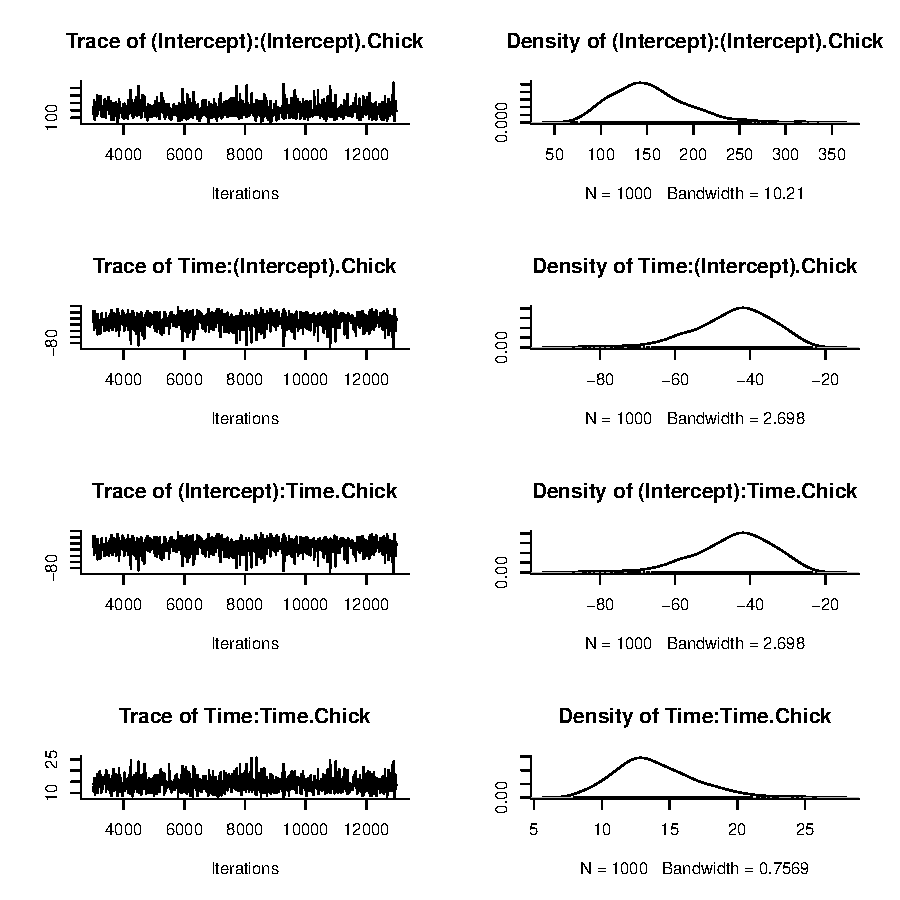
\includegraphics{Lecture4-017}
\end{center}
\caption{MCMC summary plots for the chick covariance components from model \texttt{m4a.2}. The lower and upper plots are the intercept and slope variance components respectively, and the middle two plots are the intercept-slope covariance.}
\label{RR2VCV-fig}
\end{figure}

but notice that the the estimate of intercept-slope correlation is close to the boundary of parameter space (-1):

\begin{Schunk}
\begin{Sinput}
> int.slope.cor <- m4a.2$VCV[, 2]/sqrt(m4a.2$VCV[, 1] * m4a.2$VCV[, 
+     4])
> posterior.mode(int.slope.cor)
\end{Sinput}
\begin{Soutput}
     var1 
-0.970434 
\end{Soutput}
\end{Schunk}

and shows strong autocorrelation

\begin{Schunk}
\begin{Sinput}
> autocorr(int.slope.cor)
\end{Sinput}
\begin{Soutput}
, , 1

               [,1]
Lag 0    1.00000000
Lag 10   0.15240319
Lag 50  -0.01574894
Lag 100  0.02835634
Lag 500  0.02551442
\end{Soutput}
\end{Schunk}
and we should run it for longer in order to sample the posterior adequately. For now we will carry on and obtain the predictions from the model we ran:

\begin{Schunk}
\begin{Sinput}
> W.2 <- cBind(m4a.2$X, m4a.2$Z)
> prediction.2 <- W.2 %*% posterior.mode(m4a.2$Sol)
> xyplot(weight + prediction.2@x ~ Time | Chick, data = ChickWeight)
\end{Sinput}
\end{Schunk}


\begin{figure}[!h]
\begin{center}
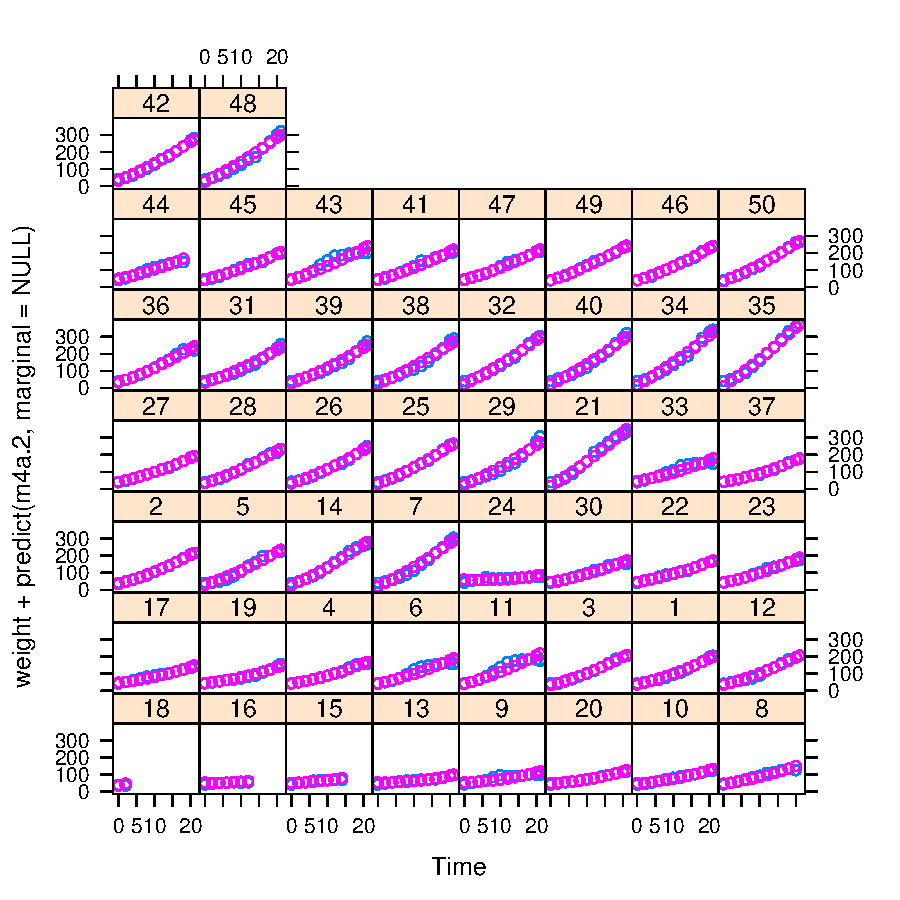
\includegraphics{Lecture4-022}
\end{center}
\caption{Weights of each chick as a function of age in blue, with the predicted weights in purple. A quadratic population growth curve was fitted with a first order random regression for chicks (i.e. a random intercept-slope model).}
\label{CWpred.2-fig}
\end{figure}

and we can see that the fit is much better (See Figure \ref{CWpred.2-fig}). In theory we could fit higher order random regressions (data and prior permitting) and use something like DIC to choose which is the best compromise between the fit of the model to the data and how many effective parameters were fitted. For example we could go from the $1^{st}$ order random regression to a $2^{nd}$ order model: 

\begin{Schunk}
\begin{Sinput}
> prior.m4a.3 <- list(R = list(V = 1, n = 0.002), G = list(G1 = list(V = diag(3), 
+     n = 3)))
> m4a.3 <- MCMCglmm(weight ~ Diet + poly(Time, 2, raw = TRUE), 
+     random = ~us(1 + poly(Time, 2, raw = TRUE)):Chick, data = ChickWeight, 
+     verbose = FALSE, pr = TRUE, prior = prior.m4a.3, saveX = TRUE, 
+     saveZ = TRUE)
\end{Sinput}
\end{Schunk}

and obtain the $3\times3$ covariance matrix:

\begin{displaymath}
{\bf V}_{{\color{red} \texttt{Chick}}}=
\left[
\begin{array}{ccc}
\sigma^{2}_{\color{blue}\texttt{(Intercept)}}&\sigma_{\color{blue}\texttt{(Intercept)}, \texttt{Time}}&\sigma_{\color{blue}\texttt{(Intercept)}, \texttt{Time$^{2}$}}\\
\sigma_{\color{blue}\texttt{(Intercept)}, \texttt{Time}}&\sigma^{2}_{\color{blue} \texttt{Time}}&\sigma_{\color{blue}\texttt{Time}, \texttt{Time$^{2}$}}\\
\sigma_{\color{blue}\texttt{(Intercept)}, \texttt{Time$^2$}}&\sigma_{\color{blue}\texttt{Time}, \texttt{Time$^{2}$}}&\sigma^{2}_{\color{blue} \texttt{Time$^2$}}\\
\end{array}
\right]
\end{displaymath}

The model predicts the chick weights to an even better degree  (See Figure \ref{CWpred.3-fig})

\begin{Schunk}
\begin{Sinput}
> W.3 <- cBind(m4a.3$X, m4a.3$Z)
> prediction.3 <- W.3 %*% posterior.mode(m4a.3$Sol)
> xyplot(weight + prediction.3@x ~ Time | Chick, data = ChickWeight)
\end{Sinput}
\end{Schunk}


\begin{figure}[!h]
\begin{center}
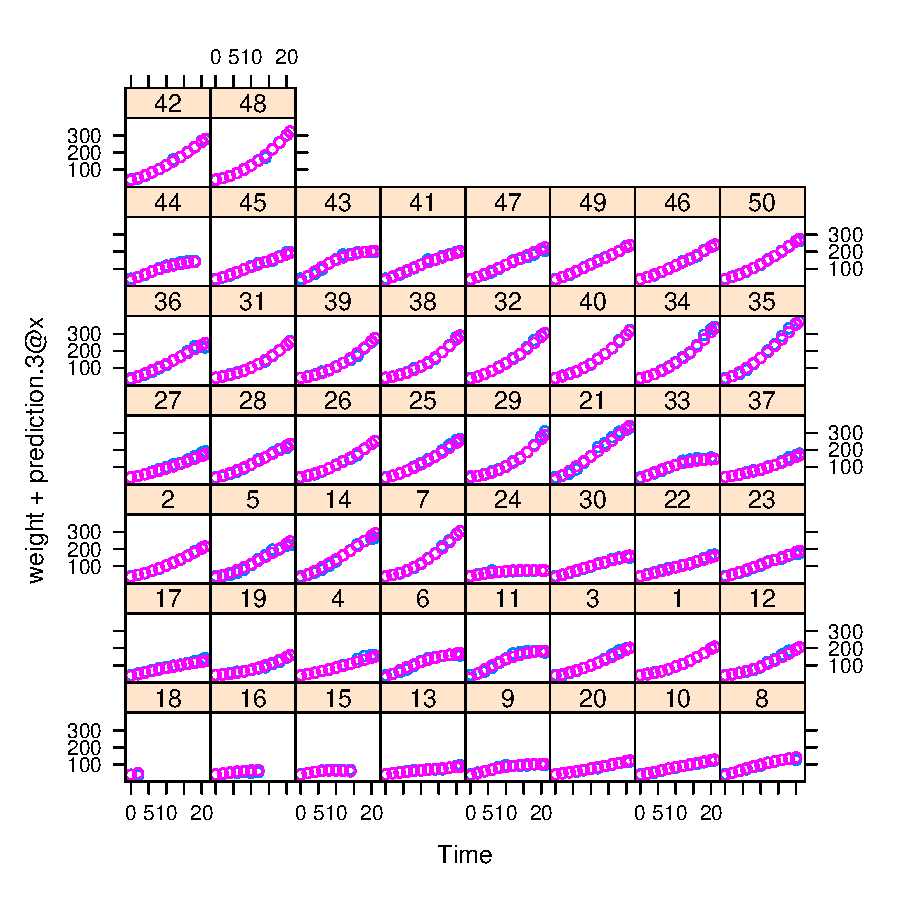
\includegraphics{Lecture4-026}
\end{center}
\caption{Weights of each chick as a function of age in blue, with the predicted weights in purple. A quadratic population growth curve was fitted with a second order random regression for chicks (i.e. a random intercept-slope-quadratic model).}
\label{CWpred.3-fig}
\end{figure}

and the DIC has gone down, suggesting that the model is better:

\begin{Schunk}
\begin{Sinput}
> m4a.1$DIC
\end{Sinput}
\begin{Soutput}
[1] 5525.705
\end{Soutput}
\begin{Sinput}
> m4a.2$DIC
\end{Sinput}
\begin{Soutput}
[1] 4544.647
\end{Soutput}
\begin{Sinput}
> m4a.3$DIC
\end{Sinput}
\begin{Soutput}
[1] 3932.791
\end{Soutput}
\end{Schunk}

It is worth seeing whether using an AIC measure using REML also suggests the highest order model is the better model. 

\begin{Schunk}
\begin{Sinput}
> library(lme4, warn.conflicts = FALSE)
> m5a.1.REML <- lmer(weight ~ Diet + poly(Time, 2, raw = TRUE) + 
+     (1 | Chick), data = ChickWeight)
> summary(m5a.1.REML)@AICtab[1]
\end{Sinput}
\begin{Soutput}
      AIC
 5578.963
\end{Soutput}
\begin{Sinput}
> m5a.2.REML <- lmer(weight ~ Diet + poly(Time, 2, raw = TRUE) + 
+     (poly(Time, 1, raw = TRUE) | Chick), data = ChickWeight)
> summary(m5a.2.REML)@AICtab[1]
\end{Sinput}
\begin{Soutput}
      AIC
 4732.387
\end{Soutput}
\begin{Sinput}
> m5a.3.REML <- lmer(weight ~ Diet + poly(Time, 2, raw = TRUE) + 
+     (poly(Time, 2, raw = TRUE) | Chick), data = ChickWeight)
> summary(m5a.3.REML)@AICtab[1]
\end{Sinput}
\begin{Soutput}
      AIC
 4274.606
\end{Soutput}
\begin{Sinput}
> detach(package:lme4)
\end{Sinput}
\end{Schunk}

\section{Expected Variances and Covariances}

Random regression models make strong assumptions about how the variance should change as a function of the predictor variable. Imagine that the intercept variance was zero, such that all regressions give the same prediction when \texttt{Time}=0. Imagine also that there was variance for slope, the predictions would look something like this:

\begin{Schunk}
\begin{Sinput}
> slope <- rnorm(30)
> plot(0, type = "n", xlim = c(-1, 1), ylim = c(-3, 3), ylab = "y", 
+     xlab = "Time")
> for (i in 1:30) {
+     lines(c(-1, 1), c(-slope[i], slope[i]))
+ }
\end{Sinput}
\end{Schunk}

\begin{figure}[!h]
\begin{center}
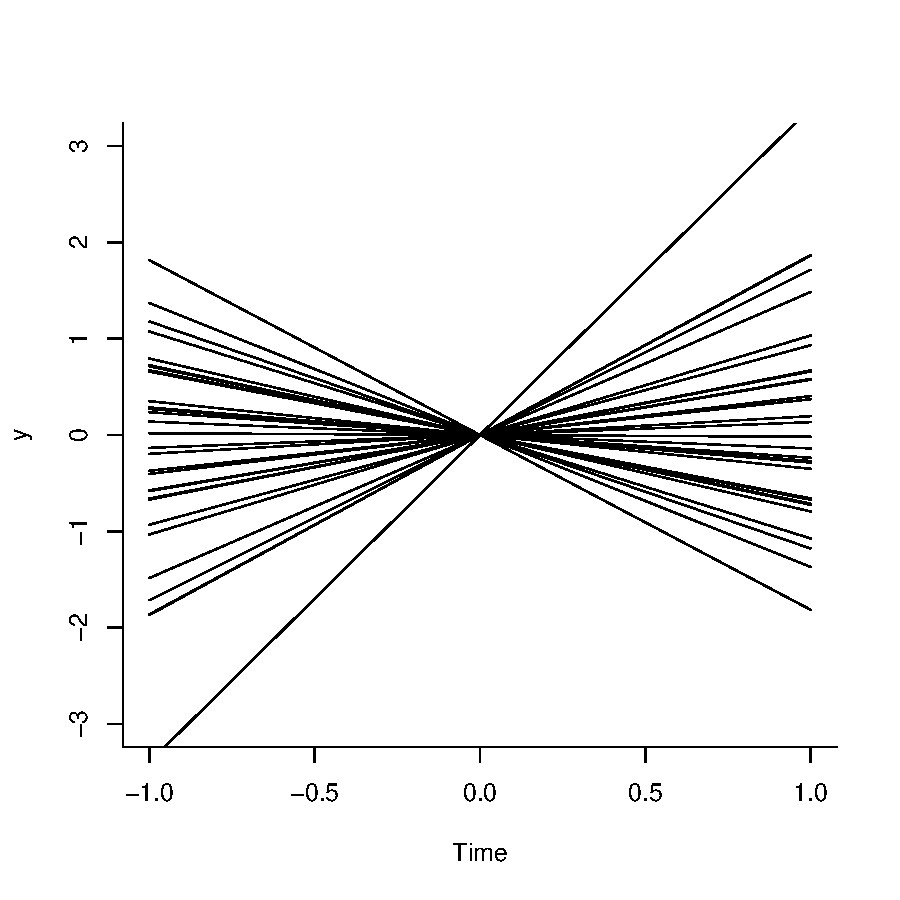
\includegraphics{Lecture4-030}
\end{center}
\caption{Hypothetical regression lines where the variance in slopes is one but the variance in intercepts is zero. The expected variance of y is a quadratic function of Time, being zero when Time=0, and increasing with positive or negative values.}
\label{RRtoy-fig}
\end{figure}


with the variance increasing at extreme values of \texttt{Time} and being zero at \texttt{Time}=0.  For an intercept-slope model such as this the expected variance is quadratic in the predictor, and for a intercept-slope-quadratic model the variance is cubic in the predictor. Generally the expected variance can be obtained using:

\begin{displaymath}
VAR[y] = \textrm{diag}({\bf Z}{\bf V}{\bf Z}^{'})
\label{RRvar-eq}
\end{displaymath}
  
and we can use this to predict the change in variance as a function of \texttt{Time} for the three models:


\begin{Schunk}
\begin{Sinput}
> pos.time <- seq(0, 21, length = 100)
> polynomial <- leg(pos.time, 2, normalized = FALSE)
> beta.1 <- c(posterior.mode(m4a.1$Sol[, 1]), posterior.mode(m4a.1$Sol[, 
+     5]), posterior.mode(m4a.1$Sol[, 6]))
> beta.2 <- c(posterior.mode(m4a.2$Sol[, 1]), posterior.mode(m4a.2$Sol[, 
+     5]), posterior.mode(m4a.2$Sol[, 6]))
> beta.3 <- c(posterior.mode(m4a.3$Sol[, 1]), posterior.mode(m4a.3$Sol[, 
+     5]), posterior.mode(m4a.3$Sol[, 6]))
> VCV.1 <- matrix(posterior.mode(m4a.1$VCV)[1], 1, 1)
> VCV.2 <- matrix(posterior.mode(m4a.2$VCV)[1:(2^2)], 2, 2)
> VCV.3 <- matrix(posterior.mode(m4a.3$VCV)[1:(3^2)], 3, 3)
> units.1 <- posterior.mode(m4a.1$VCV)[2]
> units.2 <- posterior.mode(m4a.2$VCV)[5]
> units.3 <- posterior.mode(m4a.3$VCV)[10]
\end{Sinput}
\end{Schunk}

\iftalk
\begin{Schunk}
\begin{Sinput}
> plot(weight ~ Time, data = ChickWeight, cex.lab = 1.5)
> mu.1 <- polynomial %*% beta.1
> sd.1 <- sqrt(units.1 + diag(polynomial[, 1, drop = FALSE] %*% 
+     VCV.1 %*% t(polynomial[, 1, drop = FALSE])))
> lines(mu.1 ~ pos.time, lwd = 2)
> lines(I(mu.1 + 1.96 * sd.1) ~ pos.time, lty = 2, lwd = 2)
> lines(I(mu.1 - 1.96 * sd.1) ~ pos.time, lty = 2, lwd = 2)
\end{Sinput}
\end{Schunk}
\else
\begin{Schunk}
\begin{Sinput}
> plot(weight ~ Time, data = ChickWeight)
> mu.1 <- polynomial %*% beta.1
> sd.1 <- sqrt(units.1 + diag(polynomial[, 1, drop = FALSE] %*% 
+     VCV.1 %*% t(polynomial[, 1, drop = FALSE])))
> lines(mu.1 ~ pos.time)
> lines(I(mu.1 + 1.96 * sd.1) ~ pos.time, lty = 2)
> lines(I(mu.1 - 1.96 * sd.1) ~ pos.time, lty = 2)
\end{Sinput}
\end{Schunk}
\fi

\begin{figure}[!h]
\begin{center}
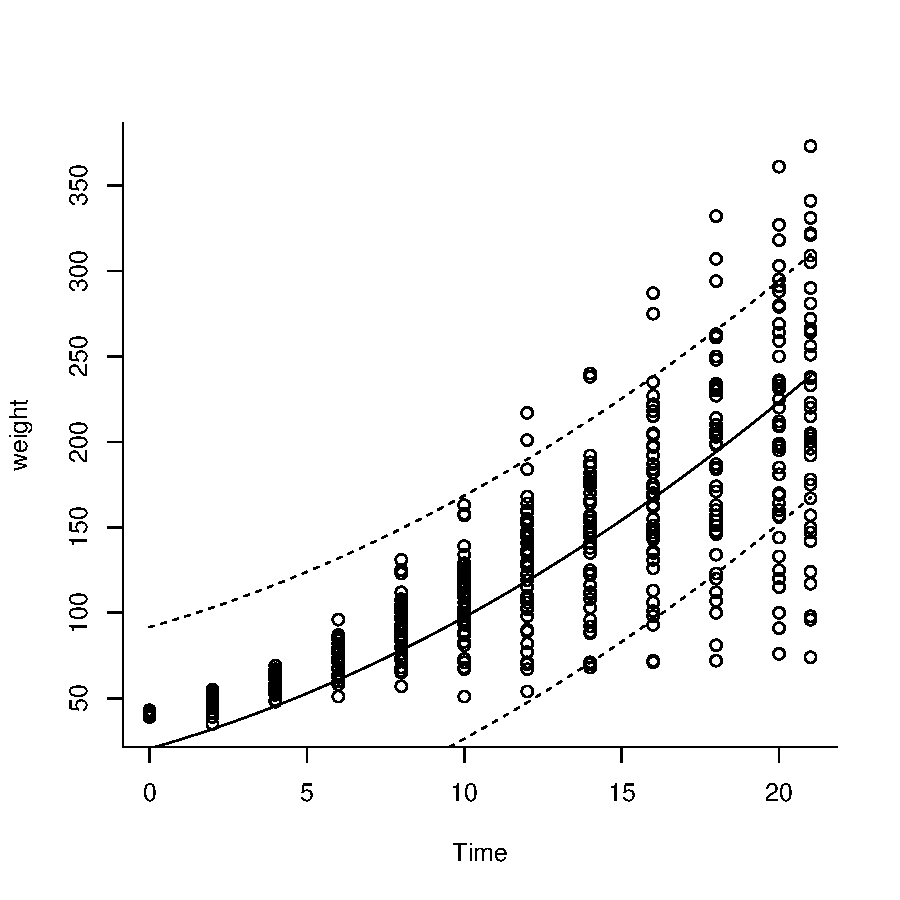
\includegraphics{Lecture4-034}
\end{center}
\caption{Chick weights plotted as a function of time. 95\% of the data are expected to fall within the dashed lines assuming the model with random intercepts is the correct model, and the diet treatments have small effects.}
\label{VCVpred.1-fig}
\end{figure}

The simple model, without a slope term has constant variance across the range, and is clearly inconsistent with the data. The second model on the other hand

\iftalk
\begin{Schunk}
\begin{Sinput}
> plot(weight ~ Time, data = ChickWeight, cex.lab = 1.5)
> mu.2 <- polynomial %*% beta.2
> sd.2 <- sqrt(units.2 + diag(polynomial[, 1:2, drop = FALSE] %*% 
+     VCV.2 %*% t(polynomial[, 1:2, drop = FALSE])))
> lines(mu.2 ~ pos.time, lwd = 2)
> lines(I(mu.2 + 1.96 * sd.2) ~ pos.time, lty = 2, lwd = 2)
> lines(I(mu.2 - 1.96 * sd.2) ~ pos.time, lty = 2, lwd = 2)
\end{Sinput}
\end{Schunk}
\else
\begin{Schunk}
\begin{Sinput}
> plot(weight ~ Time, data = ChickWeight)
> mu.2 <- polynomial %*% beta.2
> sd.2 <- sqrt(units.2 + diag(polynomial[, 1:2, drop = FALSE] %*% 
+     VCV.2 %*% t(polynomial[, 1:2, drop = FALSE])))
> lines(mu.2 ~ pos.time)
> lines(I(mu.2 + 1.96 * sd.2) ~ pos.time, lty = 2)
> lines(I(mu.2 - 1.96 * sd.2) ~ pos.time, lty = 2)
\end{Sinput}
\end{Schunk}
\fi

\begin{figure}[!h]
\begin{center}
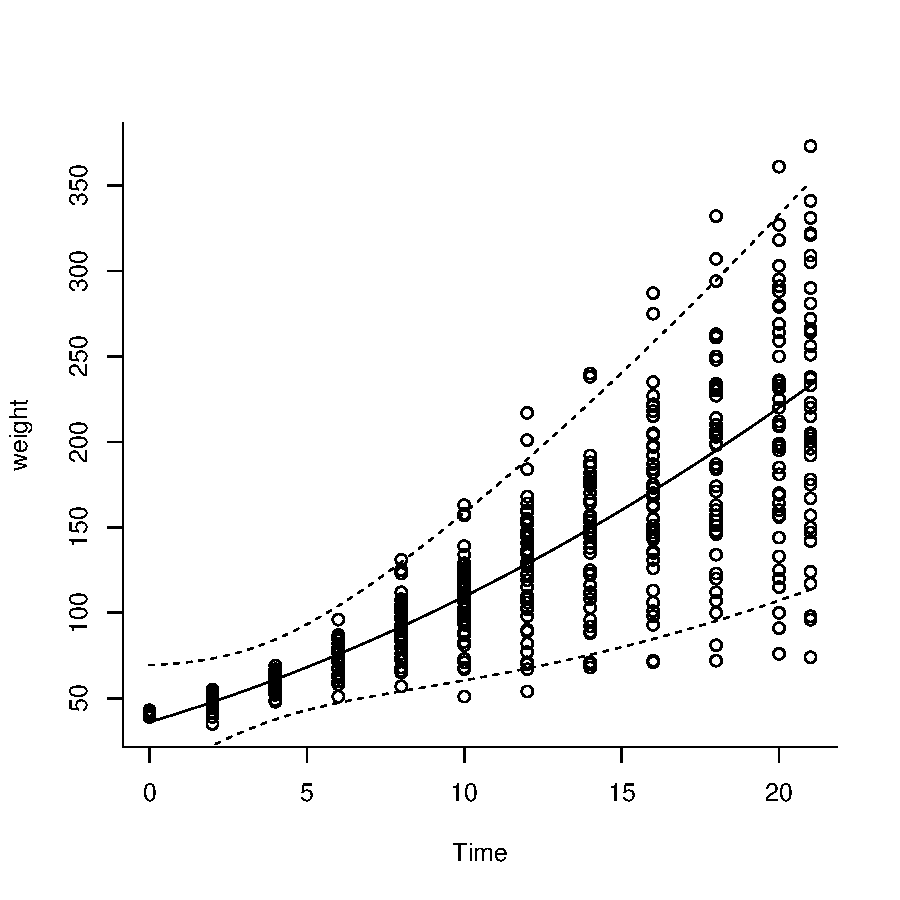
\includegraphics{Lecture4-037}
\end{center}
\caption{Chick weights plotted as a function of time. 95\% of the data are expected to fall within the dashed lines assuming the model with random intercepts and slopes is the correct model, and the diet treatments have small effects.}
\label{VCVpred.2-fig}
\end{figure}

has an expected variance structure very close to that observed. The highest order model, which was the best using information criteria such as AIC an DIC, also does badly: 

\iftalk
\begin{Schunk}
\begin{Sinput}
> plot(weight ~ Time, data = ChickWeight, ylim = c(-150, 600), 
+     cex.lab = 1.5)
> mu.3 <- polynomial %*% beta.3
> sd.3 <- sqrt(units.3 + diag(polynomial[, 1:3, drop = FALSE] %*% 
+     VCV.3 %*% t(polynomial[, 1:3, drop = FALSE])))
> lines(mu.3 ~ pos.time, lwd = 2)
> lines(I(mu.3 + 1.96 * sd.3) ~ pos.time, lty = 2, lwd = 2)
> lines(I(mu.3 - 1.96 * sd.3) ~ pos.time, lty = 2, lwd = 2)
\end{Sinput}
\end{Schunk}
\else
\begin{Schunk}
\begin{Sinput}
> plot(weight ~ Time, data = ChickWeight, ylim = c(-150, 600))
> mu.3 <- polynomial %*% beta.3
> sd.3 <- sqrt(units.3 + diag(polynomial[, 1:3, drop = FALSE] %*% 
+     VCV.3 %*% t(polynomial[, 1:3, drop = FALSE])))
> lines(mu.3 ~ pos.time)
> lines(I(mu.3 + 1.96 * sd.3) ~ pos.time, lty = 2)
> lines(I(mu.3 - 1.96 * sd.3) ~ pos.time, lty = 2)
\end{Sinput}
\end{Schunk}
\fi

\begin{figure}[!h]
\begin{center}
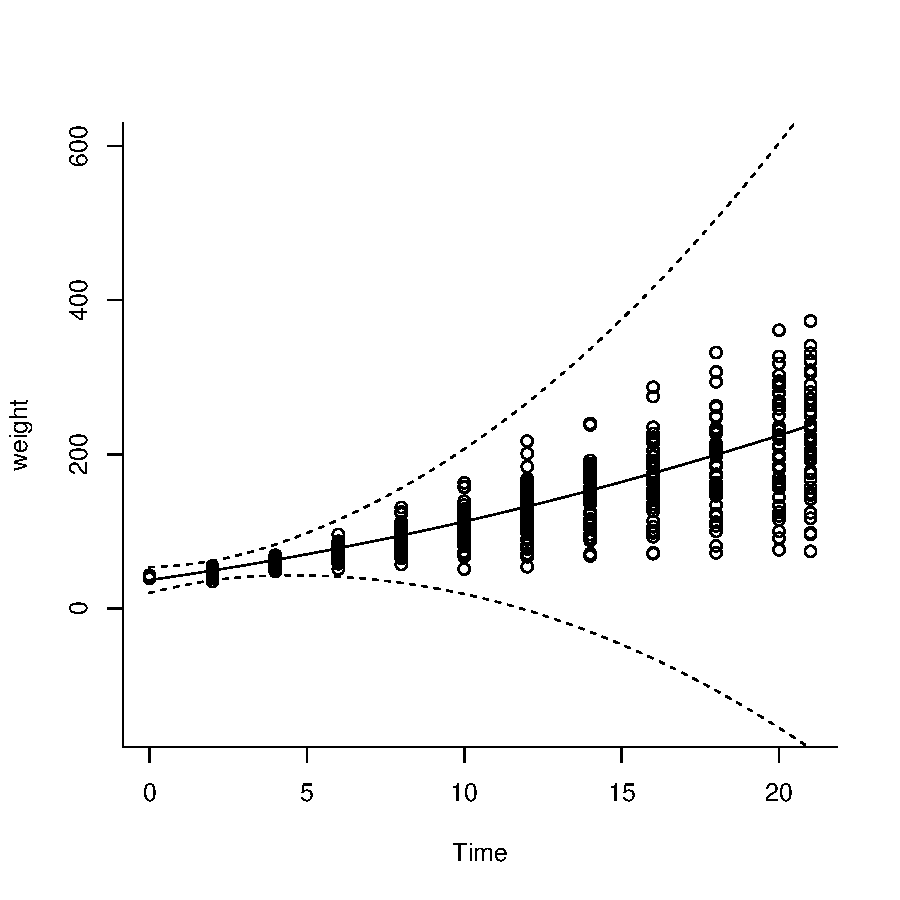
\includegraphics{Lecture4-040}
\end{center}
\caption{Chick weights plotted as a function of time. 95\% of the data are expected to fall within the dashed lines assuming the model with random intercepts, slopes and quadratic effects is the correct model, and the diet treatments have small effects.}
\label{VCVpred.3-fig}
\end{figure}

In general, I would not draw conclusions about changes in variance from random regression models \citep{Pletcher.1999a}.

\section{\texttt{us} versus \texttt{idh} and mean centring}
\label{RRcentering}
bad 
reparametersitaion

\begin{Schunk}
\begin{Sinput}
> prior.m4b.1 <- list(R = list(V = 1e-16, nu = -2), G = list(G1 = list(V = diag(2), 
+     nu = 2)))
> m4b.1 <- MCMCglmm(weight ~ Diet + poly(Time, 2, raw = TRUE), 
+     random = ~us(1 + I(Time - 3)):Chick, data = ChickWeight, 
+     verbose = FALSE, pr = TRUE, prior = prior.m4b.1, saveX = TRUE, 
+     saveZ = TRUE)
\end{Sinput}
\end{Schunk}

\section{Meta-analysis}

Random intercept-slope models implicitly assume that the variance changes as a quadratic function of the predictor. This can be used to our advantage because it allows us to fit meta-analytic models. In meta-analysis the data are usually some standardised statistic which has been estimated with different levels of measurement error. If we wanted to know the expected value of these statistics we would want to weight our answer to those measurements made with smallest amount of error.  If we assume that measurement error around the true value is normally distributed then we could assume the model:


\begin{equation}
y_{i} = \beta_{1} + m_{i} +e _{i}
\end{equation} 
 
where $\beta_{1}$ is the expected value, $m_{i}$ is some deviation due to measurement error, and $e_{i}$ is the deviation of the statistic from the global intercept not due to measurement error. Some types of meta-analysis presume $e_{i}$ does not exist and that the only variation between studies is due to measurement error. This is not realistic, I think.  Often, standard errors are reported in the literature, and these can be viewed as an approximation to the expected standard deviation of the measurement error. If we put the standard errors for each statistic as a column in the data frame (and call it \texttt{SE}) then the random term \texttt{idh(SE):units} defines a diagonal matrix with the standard errors on the diagonal. Using results from Equation \ref{RRvar-eq}


\begin{equation}
\begin{array}{rl}
\textrm{VAR}[{\bf m}] =& {\bf Z}{\bf V}{\bf Z}^{'}\\ 
               =& {\bf Z}\sigma^{2}_{m}{\bf I}{\bf Z}^{'}\\ 
               =& \sigma^{2}_{m}{\bf Z}{\bf Z}^{'}\\                               
\end{array}
\end{equation} 

fixing $\sigma^{2}_{m}=1$ in the prior, the expected variance in the measurement errors are therefore the standard errors squared (the sampling variance) and all measurement errors are assumed to be independent of each other. The random regression therefore fits a random effect meta-analysis.   

\ifalone
\bibliographystyle{jss}
\bibliography{JarLib}
\end{document}
\else
\fi


\newif\ifalone
\alonefalse
\newif\iftalk
\talkfalse

\ifalone
\documentclass{article}
\usepackage{graphicx}
\usepackage{natbib}
\usepackage{amsfonts}
\usepackage{amssymb}
\usepackage{amsthm}
\usepackage{bm}
\usepackage{Sweave}
\usepackage{lscape}
\usepackage{makeidx}
\usepackage{color}
\title{Multi-response models}

\author{Jarrod Hadfield (\texttt{j.hadfield@ed.ac.uk})}
\begin{document}
\maketitle
\else
\chapter{Multi-response models}
\label{chap5}
\fi



So far we have only fitted models to a single response variable.  Multi-response models are not that widely used, except perhaps in quantitative genetics, and deserve wider use. They allow some of the assumptions of single response models to be relaxed and can be an effective way of dealing with missing data problems. 

\section{Relaxing the univariate assumptions of causality}

Imagine we knew how much money 200 people had spent on their holiday and on their car in each of four years, and we want to know whether a relationship exists between the two.  A simple correlation would be one possibility, but then how do we control for the repeated measures? An often used solution to this problem is to choose one variable as the response (lets say the amount spent on a car) and have the other variable as a fixed covariate (the amount spent on a holiday).  The choice is essentially arbitrary, highlighting the belief that any relationship between the two types of spending maybe in part due to unmeasured variables, rather than being completely causal.\\

In practice does this matter? Lets imagine there was only one unmeasured variable: disposable income. There are repeatable differences between individuals in their disposable income, but also some variation within individuals across the four years.  Likewise, people vary in what proportion of their disposable income they are willing to spend on a holiday versus a car, but this also changes from year to year.  We can simulate some toy data to get a feel for the issues: 

\begin{Schunk}
\begin{Sinput}
> id<-gl(200,4)                  # 200 people recorded four times                      
> av_wealth<-rlnorm(200, 0, 1)               
> ac_wealth<-av_wealth[id]+rlnorm(800, 0, 1) 
> # expected disposable incomes + some year to year variation
> 
> av_ratio<-rbeta(200,10,10)                 
> ac_ratio<-rbeta(800, 2*(av_ratio[id]), 2*(1-av_ratio[id])) 
> # expected proportion spent on car + some year to year variation
> 
> y.car<-(ac_wealth*ac_ratio)^0.25     # disposable income * proportion spent on car
> y.hol<-(ac_wealth*(1-ac_ratio))^0.25 # disposable income * proportion spent on holiday                              
> Spending<-data.frame(y.hol=y.hol, y.car=y.car, id=id)
\end{Sinput}
\end{Schunk}

A simple regression suggests the two types of spending are negatively related but the association is weak with the $R^{2}=$ 0.019.

\begin{Schunk}
\begin{Sinput}
> summary(lm(y.car ~ y.hol, data = Spending))
\end{Sinput}
\begin{Soutput}
Call:
lm(formula = y.car ~ y.hol, data = Spending)

Residuals:
     Min       1Q   Median       3Q      Max 
-0.83788 -0.20558  0.00682  0.20223  1.06269 

Coefficients:
            Estimate Std. Error t value Pr(>|t|)    
(Intercept)  1.11888    0.03641  30.732  < 2e-16 ***
y.hol       -0.13460    0.03409  -3.949 8.55e-05 ***
---
Signif. codes:  0 '***' 0.001 '**' 0.01 '*' 0.05 '.' 0.1 ' ' 1 

Residual standard error: 0.2951 on 798 degrees of freedom
Multiple R-squared: 0.01917,	Adjusted R-squared: 0.01794 
F-statistic: 15.59 on 1 and 798 DF,  p-value: 8.548e-05 
\end{Soutput}
\end{Schunk}

With \texttt{id} added as a random term to deal with the the repeated measures, a similar conclusion is reached although the estimate is more negative:

\iftalk
\else
\fi

\begin{Schunk}
\begin{Sinput}
> m5a.1 <- MCMCglmm(y.car ~ y.hol, random = ~id, data = Spending, 
+     verbose = FALSE)
> summary(m5a.1$Sol[, "y.hol"])
\end{Sinput}
\begin{Soutput}
Iterations = 3001:12991
Thinning interval = 10 
Number of chains = 1 
Sample size per chain = 1000 

1. Empirical mean and standard deviation for each variable,
   plus standard error of the mean:

          Mean             SD       Naive SE Time-series SE 
    -0.1917098      0.0352772      0.0011156      0.0009755 

2. Quantiles for each variable:

   2.5%     25%     50%     75%   97.5% 
-0.2594 -0.2147 -0.1917 -0.1686 -0.1222 
\end{Soutput}
\end{Schunk}

 We may be inclined to stop there, but lets proceed with a multi-response model of the problem. The two responses are passed as a matrix using \texttt{cbind()}, and the rows of this matrix are indexed by the reserved variable {\color{red} \texttt{units}}, and the columns by the reserved variable \texttt{\color{blue} \texttt{trait}}.\\ 

It is useful to think of a new data frame where the response variables have been stacked column-wise and the other predictors duplicated accordingly. Below is the original data frame on the left (\texttt{Spending}) and the stacked data frame on the right:\\  

\begin{displaymath}
\begin{array}{cc}
\begin{array}{cccc}
&{\color{blue} \texttt{y.hol}}&{\color{blue} \texttt{y.car}}&\texttt{id}\\
{\color{red} \texttt{1}}&\texttt{1.037390}&\texttt{1.282006}&\texttt{1}\\
{\color{red} \texttt{2}}&\texttt{1.303637}&\texttt{0.648759}&\texttt{1}\\
\vdots&\vdots&\vdots\\
{\color{red} \texttt{800}}&\texttt{0.603167}&\texttt{0.964838}&\texttt{200}\\
\end{array}&
\Longrightarrow
\begin{array}{ccccc}
&\texttt{y}&{\color{blue} \texttt{trait}}&\texttt{id}&{\color{red} \texttt{units}}\\
1&\texttt{1.037390}&{\color{blue} \texttt{y.hol}}&\texttt{1}&{\color{red} \texttt{1}}\\
2&\texttt{1.303637}&{\color{blue} \texttt{y.hol}}&\texttt{1}&{\color{red} \texttt{2}}\\
\vdots&\vdots&\vdots&\vdots\\
800&\texttt{0.603167}&{\color{blue} \texttt{y.hol}}&\texttt{200}&{\color{red} \texttt{800}}\\
801&\texttt{1.282006}&{\color{blue} \texttt{y.car}}&\texttt{1}&{\color{red} \texttt{1}}\\
802&\texttt{0.648759}&{\color{blue} \texttt{y.car}}&\texttt{1}&{\color{red} \texttt{2}}\\
\vdots&\vdots&\vdots&\vdots\\
1600&\texttt{0.964838}&{\color{blue} \texttt{y.car}}&\texttt{200}&{\color{red} \texttt{800}}\\
\end{array}
\end{array}
\end{displaymath}

From this we can see that fitting a multi-response model is a direct extension to how we fitted models with categorical random interactions \ref{chap3}:

\begin{Schunk}
\begin{Sinput}
> m5a.2 <- MCMCglmm(cbind(y.hol, y.car) ~ trait - 1, random = ~us(trait):id, 
+     rcov = ~us(trait):units, data = Spending, family = c("gaussian", 
+         "gaussian"), verbose = FALSE)
\end{Sinput}
\end{Schunk}

We have fitted the fixed effect \texttt{trait} so that the two types of spending can have different intercepts. I usually suppress the intercept (\texttt{-1}) for these types of models so the second coefficient is not the difference between the intercept for the first level of \texttt{trait} (\texttt{y.hol}) and the second level (\texttt{y.car}) but the actual trait specific intercepts. In other words the design matrix for the fixed effects has the form:

\begin{displaymath}
\begin{array}{rl}
\left[
\begin{array}{cc}
\texttt{trait[1]=="y.hol"}&\texttt{trait[1]=="y.car"}\\
\texttt{trait[2]=="y.hol"}&\texttt{trait[2]=="y.car"}\\
\vdots&\vdots\\
\texttt{trait[800]=="y.hol"}&\texttt{trait[800]=="y.car"}\\
\texttt{trait[801]=="y.hol"}&\texttt{trait[801]=="y.car"}\\
\texttt{trait[802]=="y.hol"}&\texttt{trait[802]=="y.car"}\\
\vdots&\vdots\\
\texttt{trait[1600]=="y.hol"}&\texttt{trait[1600]=="y.car"}\\
\end{array}
\right]
=&
\left[
\begin{array}{cc}
1&0\\
1&0\\
\vdots&\vdots\\
1&0\\
0&1\\
0&1\\
\vdots&\vdots\\
0&1\\
\end{array}
\right]\\
\end{array}
\end{displaymath}

A $2\times2$ covariance matrix is estimated for the random term where the diagonal elements are the variance in consistent individual effects for each type of spending. The off-diagonal is the covariance between these effects which if positive suggests that people that consistently spend more on their holidays consistently spend more on their cars. A $2\times2$ residual covariance matrix is also fitted. In Section \ref{heter-sec}  we fitted heterogeneous error models using \texttt{idh():units} which made sense in this case because each level of \texttt{unit} was specific to a particular datum and so any covariances could not be estimated.   In multi-response models this is not the case because both traits have often been measured on the same observational unit and so the covariance can be measured. In the context of this example a positive covariance would indicate that in those years an individual spent a lot on their car they also spent a lot on their holiday.\\

A univariate regression is defined as the covariance between the response and the predictor divided by the variance in the predictor. We can therefore estimate a regression coefficient for these two levels of random variation, and compare them with the regression coefficient we obtained in the simpler model:
 
\begin{Schunk}
\begin{Sinput}
> id.regression <- m5a.2$VCV[, 2]/m5a.2$VCV[, 1]
> units.regression <- m5a.2$VCV[, 6]/m5a.2$VCV[, 5]
> plot(mcmc.list(m5a.1$Sol[, "y.hol"], id.regression, units.regression), 
+     density = FALSE)
\end{Sinput}
\end{Schunk}

The regression coefficients (see Figure \ref{asUV-fig})differ substantially at the within individual (green) and between individual (red) levels, and neither is entirely consistent with the regression coefficient from the univariate model (black). The process by which we generated the data gives rise to this phenomenon - large variation between individuals in their disposable income means that people who are able to spend a lot on their holiday can also afford to spend a lot on their holidays (hence a positive covariation between \texttt{id} effects). However, a person that spent a large proportion of their disposable income in a particular year on a holiday, must have less to spend that year on a car (hence a negative residual (within year) covariation). \\    



\iftalk
\else
\fi


\begin{figure}[!h]
\begin{center}
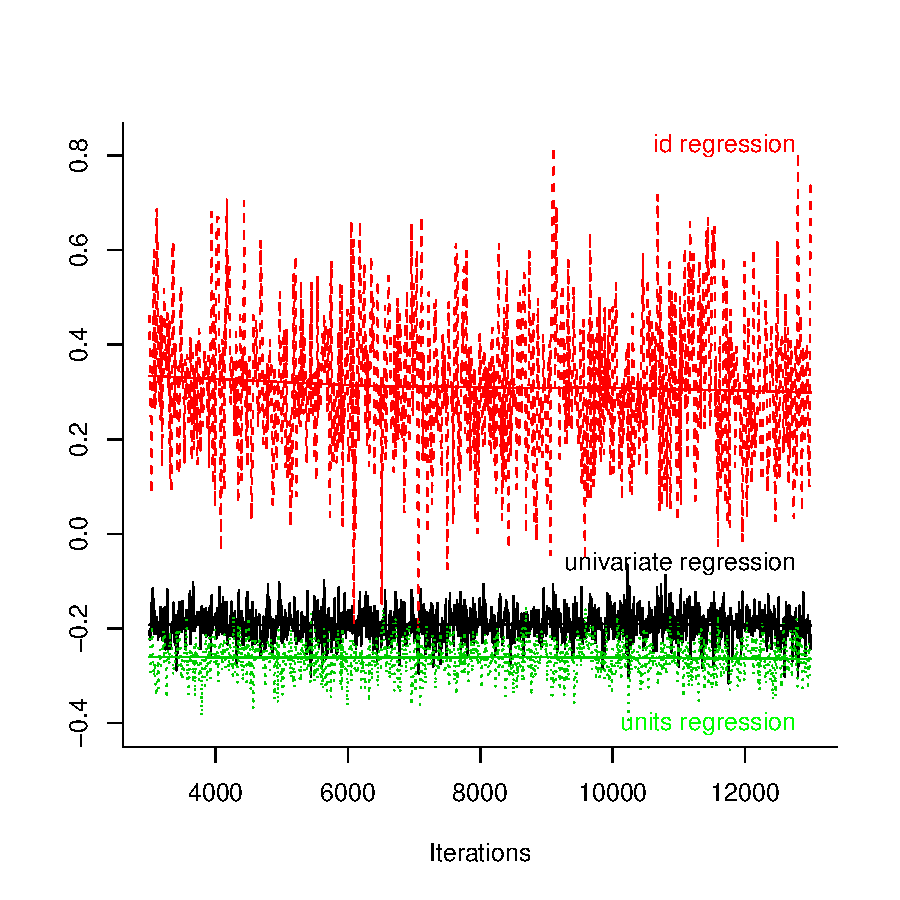
\includegraphics{Lecture5-011}
\end{center}
\caption{MCMC summary plot of the coefficient from a regression of car spending on holiday spending in black. The red and green traces are from a model where the regression coefficient is estimated at two levels: within an individual (green) and across individuals (red). The relationship between the two types of spending is in part mediating by a third unmeasured variable, disposable income.}
\label{asUV-fig}
\end{figure}

When fitting the simpler univariate model we make the assumption that the effect of spending money on a car directly effects how much you spend on a holiday. If this relationship was purely causal then all regression coefficients would have the same expectation, and the simpler model would be justified.\\

For example, we could set up a simpler model where two thirds of the variation in holiday expenditure is due to between individual differences, and holiday expenditure directly affects how much an individual will spend on their car (using a regression coefficient of -0.3). The variation in car expenditure not caused by holiday expenditure is also due to individual differences, but in this case they only explain a third of the variance.  

\begin{Schunk}
\begin{Sinput}
> Spending$y.hol2 <- rnorm(200, 0, sqrt(2))[Spending$id] + rnorm(800, 
+     0, sqrt(1))
> Spending$y.car2 <- Spending$y.hol2 * -0.3 + rnorm(200, 0, sqrt(1))[Spending$id] + 
+     rnorm(800, 0, sqrt(2))
\end{Sinput}
\end{Schunk}

We can fit the univariate and multivariate models to these data, and compare the regression coefficients as we did before. Figure \ref{MVvUV2-fig} shows that the regression coefficients are all very similar and a value of -0.3 has a reasonably high posterior probability. However, it should be noted that the posterior standard deviation is smaller in the simpler model because the more strict assumptions have allowed us to pool information across the two levels to get a more precise answer.   


\iftalk
\else
\fi
\begin{figure}[!h]
\begin{center}
\includegraphics{Lecture5-016}
\end{center}
\caption{MCMC summary plot of the coefficient from a regression of car spending on holiday spending in black. The red and green traces are from a model where the regression coefficient is estimated at two levels: within an individual (green) and across individuals (red). In this model the relationship between the two types of spending is causal and the regression coefficients have the same expectation. However, the posterior standard deviation from the simple regression is smaller because information from the two different levels is pooled.}
\label{MVvUV2-fig}
\end{figure}

\section{Multinomial Models}

Multinomial models are difficult - both to fit and interpret.  This is particularly true when each unit of observation only has a single realisation from the multinomial. In these instances the data can be expressed as a single vector of factors, and the family argument can be specified as \texttt{categorical}.  To illustrate, using a very simple example, we'll use data collected on 666 Soay sheep from the island of Hirta in the St. Kilda archipelago \citep[][Table A2.5]{Clutton-Brock.2004}. 


\begin{Schunk}
\begin{Sinput}
> data(SShorns)
> head(SShorns)
\end{Sinput}
\begin{Soutput}
  id    horn    sex
1  1 scurred female
2  2 scurred female
3  3 scurred female
4  4 scurred female
5  5  polled female
6  6  polled female
\end{Soutput}
\end{Schunk}

The sex and horn morph were recorded for each individual, giving the contingency table:  

\begin{Schunk}
\begin{Sinput}
> Ctable <- table(SShorns$horn, SShorns$sex)
> Ctable
\end{Sinput}
\begin{Soutput}
          female male
  normal      83  352
  polled      65    0
  scurred     96   70
\end{Soutput}
\end{Schunk}

and we'll see if the frequencies of the three \texttt{horn} types differ, and if the trait is sex dependent. The usual way to do this would be to use a Chi square test, and to address the first question we could add the counts of the two sexes: 

\begin{Schunk}
\begin{Sinput}
> chisq.test(rowSums(Ctable))
\end{Sinput}
\begin{Soutput}
	Chi-squared test for given probabilities

data:  rowSums(Ctable) 
X-squared = 329.5225, df = 2, p-value < 2.2e-16
\end{Soutput}
\end{Schunk}

which strongly suggests the three morphs differ in frequency. We could then ask whether the frequencies differ by sex:

\begin{Schunk}
\begin{Sinput}
> chisq.test(Ctable)
\end{Sinput}
\begin{Soutput}
	Pearson's Chi-squared test

data:  Ctable 
X-squared = 202.2962, df = 2, p-value < 2.2e-16
\end{Soutput}
\end{Schunk}

which again they do, which is not that surprising since the trait is partly sex limited, with males not expressing the polled phenotype.\\

If there were only two horn types, polled and normal for example, then we could have considered transforming the data into the binary variable \emph{polled or not?} and analysing using a glm with sex as a predictor. In doing this we have reduced the dimension of the data from $J=2$ categories to a single ($J-1=1$) contrast. The motivation for the dimension reduction is obvious; if being a male increased the probability of expressing normal horns by 10\%, it must by necessity reduce the probability of expressing polled horn type by 10\%, because an individual cannot express both horn types  simultaneously.  The dimension reduction essentially constrains the probability of expressing either horn type to unity:\\

\begin{equation}
Pr(\texttt{horn[i]}=\textrm{normal})+Pr(\texttt{horn[i]}=\textrm{polled}) = 1
\end{equation}

These concepts can be directly translated into situations with more than two categories where the unit sum constraint has the general form:

\begin{equation}
\sum_{k=1}^{J}Pr(y_{i}=k)=1 
\end{equation}

 For binary data we designated one category to be the success (polled) and one category to be the failure (normal) which we will call the baseline category.  The latent variable in this case was the log-odds ratio  of succeeding versus failing:

\begin{equation}
 l_{i} = \textrm{log}\left(\frac{Pr(\texttt{horn[i]}=\textrm{polled})}{Pr(\texttt{horn[i]}=\textrm{normal})}\right) = \textrm{logit}\left(Pr(\texttt{horn[i]}=\textrm{polled})\right)
\end{equation}

With more than two categories we need to have $J-1$ latent variables, which in the original horn type example are:

\begin{equation}
l_{i,\textrm{polled}} = \textrm{log}\left(\frac{Pr(\texttt{horn[i]}=\textrm{polled})}{Pr(\texttt{horn[i]}=\textrm{normal})}\right)
\end{equation}

and 

\begin{equation}
l_{i,\textrm{scurred}} = \textrm{log}\left(\frac{Pr(\texttt{horn[i]}=\textrm{scurred})}{Pr(\texttt{horn[i]}=\textrm{normal})}\right)
\end{equation}


The two latent variables are indexed as \texttt{trait}, and the unit of observation ($i$) as \texttt{units}, as in multi-response models. As with binary models the residual variance is not identified, and can be set to any arbitrary value. For reasons that will become clearer later I like to work with the residual covariance matrix $\frac{1}{J}({\bf I}+{\bf J})$ where  ${\bf I}$ and ${\bf J}$ are $J-1$ dimensional identity and unit matrices, respectively.

To start we will try a simple model with an intercept:\\

\begin{Schunk}
\begin{Sinput}
> IJ <- (1/3) * (diag(2) + matrix(1, 2, 2))
> prior = list(R = list(V = IJ, fix = 1))
> m5c.1 <- MCMCglmm(horn ~ trait - 1, rcov = ~us(trait):units, 
+     prior = prior, data = SShorns, family = "categorical", verbose = FALSE)
\end{Sinput}
\end{Schunk}

The posterior distribution for the intercepts is shown in Figure \ref{MN1}, and the model clearly needs to be run for longer. However...\\


\begin{figure}[!h]
\begin{center}
\includegraphics{Lecture5-024}
\end{center}
\caption{Posterior distribution of fixed effects from model \texttt{m5c.1}: a simple multinomial logit model with intercepts only}
\label{MN1}
\end{figure}



The problem can also be represented using the contrast matrix ${\bf \Delta}$ \citep{Bunch.1991}:

\begin{equation}
{\bm \Delta}=
\left[
\begin{array}{c c}
-1&-1\\
1&0\\
0&1\\
\end{array}
\right]
\end{equation}

where the rows correspond to the factor levels (\texttt{normal}, \texttt{polled} and \texttt{scurred}) and the columns to the two latent variables. For example column one corresponds to $l_{i,\textrm{polled}}$ which on the log scale is $Pr(\texttt{horn[i]}=\textrm{polled}) - Pr(\texttt{horn[i]}=\textrm{normal})$.\\

\begin{equation}
\textrm{exp}\left(({\bm \Delta}{\bm \Delta}^{'})^{-1}{\bm \Delta}{\bf l}_{i}\right) \propto E\left[\begin{array}{c} Pr(\texttt{horn[i]}=\textrm{normal})\\ Pr(\texttt{horn[i]}=\textrm{polled})\\ Pr(\texttt{horn[i]}=\textrm{scurred}) \end{array} \right]
\end{equation}

The residual and any random effect covariance matrices are for estimability purposes estimated on the $J-1$ space with  ${\bm V}={\bm \Delta}^{'}\tilde{\bf V}{\bm \Delta}$ where $\tilde{\bf V}$ is the covariance matrix estimated on the $J-1$ space. To illustrate, we will rescale the intercepts as if the residual covariance matrix was zero (see Sections and \label{pred-sec} \label{cat-sec}) and predict the expected probability for each horn type:

\begin{Schunk}
\begin{Sinput}
> Delta <- cbind(c(-1, 1, 0), c(-1, 0, 1))
> c2 <- (16 * sqrt(3)/(15 * pi))^2
> D <- ginv(Delta %*% t(Delta)) %*% Delta
> Int <- t(apply(m5c.1$Sol, 1, function(x) {
+     D %*% (x/sqrt(1 + c2 * diag(IJ)))
+ }))
> summary(mcmc(exp(Int)/rowSums(exp(Int))))
\end{Sinput}
\begin{Soutput}
Iterations = 1:1000
Thinning interval = 1 
Number of chains = 1 
Sample size per chain = 1000 

1. Empirical mean and standard deviation for each variable,
   plus standard error of the mean:

        Mean      SD  Naive SE Time-series SE
[1,] 0.65499 0.01636 0.0005173       0.001416
[2,] 0.09898 0.01090 0.0003447       0.001307
[3,] 0.24603 0.01552 0.0004909       0.001508

2. Quantiles for each variable:

        2.5%     25%     50%    75%  97.5%
var1 0.62219 0.64459 0.65481 0.6658 0.6876
var2 0.08047 0.09158 0.09833 0.1056 0.1231
var3 0.21566 0.23502 0.24585 0.2568 0.2760
\end{Soutput}
\end{Schunk}

which agrees well with those observed:

\begin{Schunk}
\begin{Sinput}
> prop.table(rowSums(Ctable))
\end{Sinput}
\begin{Soutput}
   normal    polled   scurred 
0.6531532 0.0975976 0.2492492 
\end{Soutput}
\end{Schunk}

To test for the effects of sex specific expression we can also fit a model with a sex effect:

\begin{Schunk}
\begin{Sinput}
> m5c.2 <- MCMCglmm(horn ~ trait + sex - 1, rcov = ~us(trait):units, 
+     data = SShorns, family = "categorical", prior = prior, verbose = FALSE)
\end{Sinput}
\end{Schunk}

In this case we have not interacted sex with trait, and so we are estimating the difference between the sexes in their expression of normal and polled+scurred jointly. The posterior distribution is plotted in Figure \ref{MN2} and clearly shows that males are more likely to express the normal horn phenotype than females.


\begin{figure}[!h]
\begin{center}
\includegraphics{Lecture5-029}
\end{center}
\caption{Posterior distribution of fixed effects from model \texttt{m5c.2} in which a main effect of sex was included}
\label{MN2}
\end{figure}

A more general model would be to fit estimate separate probabilities for each cell, but the contingency table indicates that one cell (polled males) has zero counts which will cause extreme separation problems. We could choose to have a better prior for the fixed effects, that is close to being flat for the two-way (i.e. polled vs scurred, normal vs.scurred \& polled vs. normal) marginal probabilities within each sex:

\begin{Schunk}
\begin{Sinput}
> prior$B = list(mu = rep(0, 4), V = kronecker(IJ, diag(2)) * (1.7 + 
+     pi^2/3))
> m5c.3 <- MCMCglmm(horn ~ at.level(sex, 1):trait + at.level(sex, 
+     2):trait - 1, rcov = ~us(trait):units, data = SShorns, family = "categorical", 
+     prior = prior, verbose = FALSE)
\end{Sinput}
\end{Schunk}

The female specific probabilities appear reasonable:

\begin{Schunk}
\begin{Sinput}
> Int <- t(apply(m5c.3$Sol[, 1:2], 1, function(x) {
+     D %*% (x/sqrt(1 + c2 * diag(IJ)))
+ }))
> summary(mcmc(exp(Int)/rowSums(exp(Int))))
\end{Sinput}
\begin{Soutput}
Iterations = 1:1000
Thinning interval = 1 
Number of chains = 1 
Sample size per chain = 1000 

1. Empirical mean and standard deviation for each variable,
   plus standard error of the mean:

       Mean      SD  Naive SE Time-series SE
[1,] 0.3513 0.03044 0.0009626       0.002997
[2,] 0.2595 0.02691 0.0008511       0.002388
[3,] 0.3892 0.02879 0.0009105       0.003235

2. Quantiles for each variable:

       2.5%    25%    50%    75%  97.5%
var1 0.2958 0.3297 0.3513 0.3724 0.4097
var2 0.2103 0.2405 0.2588 0.2775 0.3132
var3 0.3362 0.3697 0.3884 0.4079 0.4440
\end{Soutput}
\end{Schunk}

compared to the observed frequencies:

\begin{Schunk}
\begin{Sinput}
> prop.table(Ctable[, 1])
\end{Sinput}
\begin{Soutput}
   normal    polled   scurred 
0.3401639 0.2663934 0.3934426 
\end{Soutput}
\end{Schunk}

as do the male probabilities:

\begin{Schunk}
\begin{Sinput}
> Int <- t(apply(cbind(m5c.3$Sol[, 3:4]), 1, function(x) {
+     D %*% (x/sqrt(1 + c2 * diag(IJ)))
+ }))
> summary(mcmc(exp(Int)/rowSums(exp(Int))))
\end{Sinput}
\begin{Soutput}
Iterations = 1:1000
Thinning interval = 1 
Number of chains = 1 
Sample size per chain = 1000 

1. Empirical mean and standard deviation for each variable,
   plus standard error of the mean:

         Mean       SD  Naive SE Time-series SE
[1,] 0.826652 0.017969 0.0005682      0.0021322
[2,] 0.006973 0.003691 0.0001167      0.0004824
[3,] 0.166374 0.018085 0.0005719      0.0021722

2. Quantiles for each variable:

         2.5%      25%      50%      75%   97.5%
var1 0.787082 0.816109 0.827407 0.838409 0.86170
var2 0.002533 0.004268 0.005882 0.008674 0.01600
var3 0.131223 0.154416 0.165888 0.177355 0.20649
\end{Soutput}
\end{Schunk}

compared to the observed frequencies:

\begin{Schunk}
\begin{Sinput}
> prop.table(Ctable[, 2])
\end{Sinput}
\begin{Soutput}
   normal    polled   scurred 
0.8341232 0.0000000 0.1658768 
\end{Soutput}
\end{Schunk}


\section{Zero-inflated Models}

Each datum in a zero-inflated model is associated with two latent variables. The first latent variable is associated with the named distribution and the second latent variable is associated with zero inflation. I'll work through a zero-inflated Poisson (ZIP) model to make things clearer. As the name suggests, a ZIP distribution is a Poisson distribution with extra zero's. The observed zeros are modelled as a mixture distribution of zero's originating form the Poisson process and zero's arising through zero-inflation. It is the probability (on the logit scale) that a zero is from the zero-inflation process that we aim to model with the second latent variable. The likelihood has the form:

\begin{equation} 
\begin{array}{rl}
Pr(y | y=0) =& \texttt{plogis}(l_{2})+\texttt{plogis}(-l_{2})\ast \texttt{dpois}(0, \texttt{exp}(l_{1}))\\
Pr(y | y>0) =& \texttt{plogis}(-l_{2})\ast \texttt{dpois}(y, \texttt{exp}(l_{1}))\\
\end{array}
\end{equation}


{\bf pscl} fits zero-inflated models very well through the \texttt{zeroinfl} function, and I strongly recommend using it if you do not want to fit random effects. To illustrate the syntax for fitting ZIP models in MCMCglmm I will take one of their examples:   

\begin{Schunk}
\begin{Sinput}
> data("bioChemists", package = "pscl")
> head(bioChemists)
\end{Sinput}
\begin{Soutput}
  art   fem     mar kid5  phd ment
1   0   Men Married    0 2.52    7
2   0 Women  Single    0 2.05    6
3   0 Women  Single    0 3.75    6
4   0   Men Married    1 1.18    3
5   0 Women  Single    0 3.75   26
6   0 Women Married    2 3.59    2
\end{Soutput}
\end{Schunk}

\texttt{art} is the response variable - the number of papers published by a Ph.D student - and the remaining variables are to be fitted as fixed effects.  Naively, we may expect zero-inflation to be a problem given  30\% of the data are zeros, and based on the global mean we only expect around 18\%.

\begin{Schunk}
\begin{Sinput}
> table(bioChemists$art == 0)
\end{Sinput}
\begin{Soutput}
FALSE  TRUE 
  640   275 
\end{Soutput}
\begin{Sinput}
> ppois(0, mean(bioChemists$art))
\end{Sinput}
\begin{Soutput}
[1] 0.1839859
\end{Soutput}
\end{Schunk}

As with binary models we do not observe any residual variance for the zero-inflated process, and in addition the residual covariance between the zero-inflation and the Poisson process cannot be estimated because both processes cannot be observed in a single data point. To deal with this I've fixed the residual variance for the zero-inflation at 1, and the covariance is set to zero using the idh structure. Setting \texttt{V=diag(2)} and \texttt{nu=0.002}\footnote{Earlier versions of the CourseNotes had \texttt{nu=1.002}. In versions $<$2.05 the marginal prior of a variance associated with an \texttt{idh} structure was inverse-Wishart with $\texttt{nu}^{\ast}=\texttt{nu}-1$ where $\texttt{nu}^{\ast}$ is the marginal degree of belief. In versions $>=$2.05 I changed this so that $\texttt{nu}^{\ast}=\texttt{nu}$ as it was leading to confusion.} we have the inverse-gamma prior with \texttt{shape=scale=0.001} for the residual component of the Poisson process which captures over-dispersion:

\begin{Schunk}
\begin{Sinput}
> prior.m5d.1 = list(R = list(V = diag(2), nu = 0.002, fix = 2))
> m5d.1 <- MCMCglmm(art ~ trait - 1 + at.level(trait, 1):fem + 
+     at.level(trait, 1):mar + at.level(trait, 1):kid5 + at.level(trait, 
+     1):phd + at.level(trait, 1):ment, rcov = ~idh(trait):units, 
+     data = bioChemists, prior = prior.m5d.1, family = "zipoisson", 
+     verbose = FALSE)
\end{Sinput}
\end{Schunk}

As is often the case the parameters of the zero-inflation model mixes poorly (See Figure \ref{ZIP}) especially when compared to equivalent hurdle models (See Section \ref{Hurdle}). Poor mixing is often associated with distributions that may \emph{not} be zero-inflated but instead over-dispersed.\\  


\begin{figure}[!h]
\begin{center}
\includegraphics{Lecture5-039}
\end{center}
\caption{Posterior distribution of fixed effects from model \texttt{m5d.1} in which trait 1 (\texttt{art}) is the Poisson process and trait 2 (\texttt{zi.art}) is the zero-inflation.}
\label{ZIP}
\end{figure}

The model would have to be run for (much) longer to say something concrete about the level of zero-inflation but my guess would be it's not a big issue, given the probability is probably quite small:

\begin{Schunk}
\begin{Sinput}
> quantile(plogis(m5d.1$Sol[, 2]/sqrt(1 + c2)))
\end{Sinput}
\begin{Soutput}
         0%         25%         50%         75%        100% 
0.002621302 0.006396358 0.008289576 0.010693291 0.016856108 
\end{Soutput}
\end{Schunk}

\subsection{Posterior predictive checks}

Another useful check is to fit the standard Poisson model and use posterior predictive checks to see how many zero's you would expect under the simple model:

\begin{Schunk}
\begin{Sinput}
> prior.m5d.2 = list(R = list(V = diag(1), nu = 0.002))
> m5d.2 <- MCMCglmm(art ~ fem + mar + kid5 + phd + ment, data = bioChemists, 
+     prior = prior.m5d.2, family = "poisson", saveX = TRUE, verbose = FALSE)
> nz <- 1:1000
> oz <- sum(bioChemists$art == 0)
> for (i in 1:1000) {
+     pred.l <- rnorm(915, (m5d.2$X %*% m5d.2$Sol[i, ])@x, sqrt(m5d.2$VCV[i]))
+     nz[i] <- sum(rpois(915, exp(pred.l)) == 0)
+ }
\end{Sinput}
\end{Schunk}

Figure \ref{PPZIP}  shows a histogram of the posterior predictive distribution of zero's from the model (\texttt{nz}) compared to the observed number of zeros (\texttt{oz}). The simpler model seems to be consistent with the data, suggesting that a ZIP model may not be required.


\begin{figure}[!h]
\begin{center}
\includegraphics{Lecture5-043}
\end{center}
\caption{Posterior predictive distribution of zeros from model \texttt{m5d.2} with the observed number in red.}
\label{PPZIP}
\end{figure}

\section{Hurdle Models}
\label{Hurdle}

Hurdle models are very similar to zero-inflated models but they can be used to model zero-deflation as well as zero-inflation and seem to have much better mixing properties.  As in ZIP models each datum in the hurdle model is associated with two latent variables. However, whereas in a ZIP model the first latent variable is the mean parameter of a Poisson distribution the equivalent latent variable in the hurdle model is the mean parameter of a zero-truncated Possion distribution (i.e. a Poisson distribution without the zeros  observed). In addition the second latent variable in a ZIP model is the probability that an observed zero is due to zero-inflation rather than the Poisson process. In hurdle models the second latent variable is simply the probability (on the logit scale) that the response variable is zero or not. The likelihood is:

\begin{equation} 
\begin{array}{rl}
Pr(y | y=0) =& \texttt{plogis}(l_{2})\\
Pr(y | y>0) =& \texttt{plogis}(-l_{2})\ast \texttt{dpois}(y, \texttt{exp}(l_{1}))/(1-\texttt{ppois}(0, \texttt{exp}(l_{1})))\\
\end{array}
\end{equation}

 To illustrate, we will refit the ZIP model (\texttt{m5d.1}) as a hurdle-Poisson model.

\begin{Schunk}
\begin{Sinput}
> m5d.3 <- MCMCglmm(art ~ trait - 1 + at.level(trait, 1):fem + 
+     at.level(trait, 1):mar + at.level(trait, 1):kid5 + at.level(trait, 
+     1):phd + at.level(trait, 1):ment, rcov = ~idh(trait):units, 
+     data = bioChemists, prior = prior.m5d.1, family = "hupoisson", 
+     verbose = FALSE)
\end{Sinput}
\end{Schunk}

Plotting the Markov chain for the equivalent parameters that were plotted for the ZIP model shows that the mixing properties are much better (compare Figure \ref{ZIP} with Figure \ref{HU}).


\begin{figure}[!h]
\begin{center}
\includegraphics{Lecture5-046}
\end{center}
\caption{Posterior distribution of fixed effects from model \texttt{m5d.3} in which trait 1 (\texttt{art}) is the zero-truncated Poisson process and trait 2 (\texttt{hu.art}) is the binary trait zero or non-zero.}
\label{HU}
\end{figure}

The interpretation of the model is slightly different. Fitting just an intercept in the hurdle model implies that the proportion of zeros observed across different combinations of those fixed effects fitted for the Poisson process is constant. Our 95\% credible intervals for this proportion is (See section \ref{pred-sec}):

\begin{Schunk}
\begin{Sinput}
> c2 <- (16 * sqrt(3)/(15 * pi))^2
> HPDinterval(plogis(m5d.3$Sol[, 2]/sqrt(1 + c2)))
\end{Sinput}
\begin{Soutput}
         lower     upper
var1 0.2639715 0.3228268
attr(,"Probability")
[1] 0.95
\end{Soutput}
\end{Schunk}

and we can compare this to the predicted number of zero's from the Poisson process if it had not been zero-truncated:

\begin{Schunk}
\begin{Sinput}
> HPDinterval(ppois(0, exp(m5d.3$Sol[, 1] + 0.5 * m5d.3$VCV[, 1])))
\end{Sinput}
\begin{Soutput}
         lower     upper
var1 0.1416241 0.3596839
attr(,"Probability")
[1] 0.95
\end{Soutput}
\end{Schunk}

The credible intervals largely overlap, strongly suggesting a standard Poisson model would be adequate. However, our prediction for the number of zero's that would arise form a non-truncated Poisson process only involved the intercept term. This prediction therefore pertains to the number of articles published by single women with no young children who obtained their Ph.D's from departments scoring zero for prestige (\texttt{phd}) and whose mentors had published nothing in the previous 3 years.  Our equivalent prediction for men is a little lower 

\begin{Schunk}
\begin{Sinput}
> HPDinterval(ppois(0, exp(m5d.3$Sol[, 1] + m5d.3$Sol[, 3] + 0.5 * 
+     m5d.3$VCV[, 1])))
\end{Sinput}
\begin{Soutput}
         lower     upper
var1 0.0939242 0.2982136
attr(,"Probability")
[1] 0.95
\end{Soutput}
\end{Schunk}

suggesting that perhaps the number of zero's is greater than we expected for this group. However, this may just be a consequence of us fixing the proportion of zero's to be constant across these groups. We can relax this assumption by fitting a separate term for the proportion of zeros for men:

\begin{Schunk}
\begin{Sinput}
> m5d.4 <- MCMCglmm(art ~ trait - 1 + at.level(trait, 1:2):fem + 
+     at.level(trait, 1):mar + at.level(trait, 1):kid5 + at.level(trait, 
+     1):phd + at.level(trait, 1):ment, rcov = ~idh(trait):units, 
+     data = bioChemists, prior = prior.m5d.1, family = "hupoisson", 
+     verbose = FALSE)
\end{Sinput}
\end{Schunk}

which reveals that although this proportion is expected to be (slightly) smaller: 


\begin{Schunk}
\begin{Sinput}
> HPDinterval(plogis((m5d.4$Sol[, 2] + m5d.4$Sol[, 4])/sqrt(1 + 
+     c2)))
\end{Sinput}
\begin{Soutput}
         lower     upper
var1 0.2310072 0.3085805
attr(,"Probability")
[1] 0.95
\end{Soutput}
\end{Schunk}


the proportion of zeros expected for men is probably still less than what we expect from a non-truncated Poisson process for which the estimates have changed very little:

\begin{Schunk}
\begin{Sinput}
> HPDinterval(ppois(0, exp(m5d.4$Sol[, 1] + m5d.4$Sol[, 3] + 0.5 * 
+     m5d.4$VCV[, 1])))
\end{Sinput}
\begin{Soutput}
          lower     upper
var1 0.08556727 0.2451435
attr(,"Probability")
[1] 0.95
\end{Soutput}
\end{Schunk}


This highlights one of the disadvantages of hurdle models. If explanatory variables have been fitted that affect the expectation of the Poisson process than this implies that the proportion of zero's observed will also vary across these same explanatory variables, even in the absence of zero-inflation. It may then be necessary to fit an equally complicated model for both processes even though a single parameter would suffice in a ZIP model. However, in the absence of zero-inflation the intercept of the zero-inflation process in a ZIP model is $-\infty$ on the logit scale causing numerical and inferential problems. An alternative model are zero-altered models. 

\section{Zero-altered Models}
\label{ZAP}

Zero-altered Poisson (ZAP) models are identical to Poisson-hurdle models except a complementary log-log link is used instead of the logit link when modeling the proportion of zeros. However for reasons that will become clearer below, the zero-altered process (\texttt{za}) is predicting non-zeros as opposed to the ZIP and hurdle-Poisson models where it is the number of zeros.  The likelihood is:

\begin{equation} 
\begin{array}{rl}
Pr(y | y=0) =& 1-\texttt{pexp}(\texttt{exp}(l_{2}))\\
Pr(y | y>0) =& \texttt{pexp}(\texttt{exp}(l_{2}))\ast \texttt{dpois}(y, \texttt{exp}(l_{1}))/(1-\texttt{ppois}(0, \texttt{exp}(l_{1})))\\
\end{array}
\end{equation}

since the inverse of the complementary log-log transformation is the distribution function of the extreme value (log-exponential) distribution.\\

It happens that $\texttt{ppois}(0,\texttt{exp}(l)) = \texttt{dpois}(0,\texttt{exp}(l)) = 1-\texttt{pexp}(\texttt{exp}(l))$ so that if $l = l_{1} = l_{2}$ then the likelihood reduces to:

\begin{equation} 
\begin{array}{rl}
Pr(y | y=0) =& \texttt{dpois}(0,\texttt{exp}(l))\\
Pr(y | y>0) =& \texttt{dpois}(y, \texttt{exp}(l))\\
\end{array}
\end{equation}

which is equivalent to a standard Poisson model.\\

We can then test for zero-flation by constraining the over-dispersion to be the same for both process using a \texttt{trait} by \texttt{units} interaction in the R-structure, and by setting up the contrasts so that the zero-altered regression coefficients are expressed as differences from the Poisson regression coefficients. When this difference is zero the variable causes no zero-flation, when it is negative it causes zero-inflation and when it is positive it causes zero-deflation:
  
\begin{Schunk}
\begin{Sinput}
> m5d.5 <- MCMCglmm(art ~ trait + trait:(fem + mar + kid5 + phd + 
+     ment), rcov = ~trait:units, data = bioChemists, family = "zapoisson", 
+     verbose = FALSE)
> summary(m5d.5)
\end{Sinput}
\begin{Soutput}
 Iterations = 12991
 Thinning interval  = 3001
 Sample size  = 1000 

 DIC: 3040.044 

 R-structure:  ~trait:units

            post.mean l-95% CI u-95% CI eff.samp
trait:units    0.3513   0.2556   0.4511    64.04

 Location effects: art ~ trait + trait:(fem + mar + kid5 + phd + ment) 

                       post.mean  l-95% CI  u-95% CI eff.samp  pMCMC    
(Intercept)             0.369879  0.067267  0.690729    362.9  0.018 *  
traitza_art            -0.599152 -1.194254 -0.068890    200.4  0.030 *  
traitart:femWomen      -0.198237 -0.376178 -0.044519    300.0  0.008 ** 
traitza_art:femWomen   -0.148079 -0.387571  0.053130    216.0  0.172    
traitart:marMarried     0.082681 -0.090349  0.273456    305.8  0.356    
traitza_art:marMarried  0.236665 -0.012941  0.484367    191.3  0.066 .  
traitart:kid5          -0.129367 -0.262294  0.007003    111.3  0.052 .  
traitza_art:kid5       -0.196143 -0.359391 -0.046256    238.4  0.012 *  
traitart:phd            0.007502 -0.072980  0.095214    350.4  0.846    
traitza_art:phd         0.029532 -0.088120  0.135599    197.5  0.560    
traitart:ment           0.019675  0.012432  0.026540    386.9 <0.001 ***
traitza_art:ment        0.047845  0.035106  0.062712    112.5 <0.001 ***
---
Signif. codes:  0 '***' 0.001 '**' 0.01 '*' 0.05 '.' 0.1 ' ' 1 
\end{Soutput}
\end{Schunk}

we can see from this that having kids causes `significant' zero-inflation and the more papers a mentor produces, the more zero-deflation (or conversely the less papers a mentor produces, the more zero-inflation).

\ifalone
\end{document}
\else
\fi


\newif\ifalone
\alonefalse
\ifalone
\documentclass{article}
\usepackage{graphicx}
\usepackage{natbib}
\usepackage{amsfonts}
\usepackage{amssymb}
\usepackage{amsthm}
\usepackage{bm}
\usepackage{Sweave}
\usepackage{lscape}
\usepackage{makeidx}


\title{Pedigrees and Phylogenies}

\author{Jarrod Hadfield (\texttt{j.hadfield@ed.ac.uk})}
\begin{document}
\maketitle
\else
\chapter{Pedigrees and Phylogenies}
\label{chap6}
\fi
\begin{Schunk}
\begin{Sinput}
> library(kinship)
\end{Sinput}
\end{Schunk}



Pedigrees and phylogenies are similar things: they are both ways of representing shared ancestry. Under a quantitative genetic model of inheritance, or a Brownian motion model of evolution, GLMM's can be readily extended to model the similarities that exist between the phenotypes of related individuals or taxa.  In the context of quantitative genetics these models are known as `animal' models \citep{Henderson.1976}, and in the context of the comparative method these models are known as phylogenetic mixed models \citep{Lynch.1991}. The two models are almost identical, and are relatively minor modifications to the basic mixed model \citep{Hadfield.2010b}. 


\section{Pedigree and phylogeny formats}

\subsection{Pedigrees}

\texttt{MCMCglmm} handles pedigrees stored in 3-column tabular form, with each row representing a single individual. The first column should contain the unique identifier of the individual, and columns 2 and 3 should be the unique identifiers of the individual's parents. Parents must appear before their offspring in the table. I usually have the dam (mother) in the first column and the sire (father) in the third. I prefer the words dam and sire because if I subscript things with $m$ and $f$ I can never remember whether I mean male and female, or mother and father. In hermaphrodite systems the same individual may appear in both columns, even within the same row if an individual was produced through selfing.  This is not a problem, but \texttt{MCMCglmm} will issue a warning in case hermaphrodites are not present and a data entry mistake has been made. Impossible pedigrees (for example individual's that give birth to their own mother) are a problem and \texttt{MCMCglmm} will issue an error, hopefully with an appropriate message, when impossibilities are detected.\\

If the parent(s) of an individual are unknown then a missing value (\texttt{NA}) should be assigned in the relevant column. All individuals appearing as dams or sires need to have their own record, even if both of their parents are unknown. Often the number of individuals in a pedigree will be greater than the number of individuals for which phenotypic data exist. \texttt{MCMCglmm} can handle this, as long as all the individuals appearing in the data frame passed to \texttt{data} also appear in the pedigree.\\
   
To illustrate, we can load a pedigree for a population of blue tits and display the pedigree for the nuclear family that has individuals \texttt{"R187920"} and \texttt{"R187921"} as parents:

\begin{Schunk}
\begin{Sinput}
> data(BTped)
> Nped <- BTped[which(apply(BTped, 1, function(x) {
+     any(x == "R187920" | x == "R187921")
+ })), ]
> Nped
\end{Sinput}
\begin{Soutput}
      animal     dam    sire
66   R187920    <NA>    <NA>
172  R187921    <NA>    <NA>
325  R187726 R187920 R187921
411  R187724 R187920 R187921
503  R187723 R187920 R187921
838  R187613 R187920 R187921
932  R187612 R187920 R187921
1030 R187609 R187920 R187921
\end{Soutput}
\end{Schunk}

Both parents form part of what is known as the base population - they are outbred and unrelated to anybody else in the pedigree.\\

\texttt{MCMCglmm} and \texttt{MasterBayes} have several pedigree manipulation functions. (\texttt{MasterBayes::orderPed})  orders a pedigree so parents appear before their offspring, (\texttt{MasterBayes::insertPed}) inserts records for individuals that only appear as parents (or a vector of specified individuals).  When the number of individuals with phenotypic data is less than the number of individuals in the pedigree it is sometimes possible to remove uninformative individuals from the pedigree and thus reduce the computation time. This is known as pruning the pedigree and is implemented in the  \texttt{MCMCglmm} function \texttt{prunePed}. A vector of measured individuals is specified in the argument \texttt{keep} and specifying \texttt{make.base=TRUE} implements the most complete pruning. Note,  \texttt{make.base=FALSE} is the default argument so you'll need to explicitly specify \texttt{TRUE} in the call to  \texttt{prunePed}. Michael Morrissey's \texttt{pedantics} package, and the \texttt{kinship} package also have many other useful pedigree orientated functions. In fact, the \texttt{orderPed} function in \texttt{MasterBayes} is built around functions provided by  \texttt{kinship}.\\

\subsection{Phylogenies}

Phylogenies can be expressed in tabular form, although only two columns are required because each species only has a single parent. In general however,  phylogenies are not expressed in this form presumably because it is hard to traverse phylogenies (and pedigrees) backwards in time when they are stored this way. For phylogenetic mixed models we generally only need to traverse phylogenies forward in time (if at all) but I have stuck with convention and used the \texttt{phylo} class from the \texttt{ape} package to store phylogenies.  As with pedigrees, all species appearing in the data frame passed to \texttt{data} need to appear in the phylogeny. Typically, this will only include species at the tips of the phylogeny and so the measured species should appear in the \texttt{tip.label} element of the phylo object. An error message will be issued if this is not the case. Data may also exist for ancestral species, or even for species present at the tips but measured many generations before. It is possible to include these data as long as the phylogeny has labelled internal nodes. If nodes are unlabeled then  \texttt{MCMCglmm}  names them internally using the default arguments of   \texttt{makeNodeLabel} from \texttt{ape}.\\ 

To illustrate, lets take the phylogeny of bird families included in the \texttt{ape} package, and extract the phylogeny in tabular form for the Paridae (Tits), Certhiidae (Treecreepers), Gruidae (Cranes) and the Struthionidae (Ostriches):

\begin{Schunk}
\begin{Sinput}
> data("bird.families")
> bird.families <- makeNodeLabel(bird.families)
> some.families <- c("Certhiidae", "Paridae", "Gruidae", "Struthionidae")
> Nphylo <- drop.tip(bird.families, setdiff(bird.families$tip.label, 
+     some.families))
> INphylo <- inverseA(Nphylo)
> INphylo$pedigree
\end{Sinput}
\begin{Soutput}
     node.names                  
[1,] "Node58"        NA        NA
[2,] "Node122"       "Node58"  NA
[3,] "Struthionidae" NA        NA
[4,] "Gruidae"       "Node58"  NA
[5,] "Certhiidae"    "Node122" NA
[6,] "Paridae"       "Node122" NA
\end{Soutput}
\end{Schunk}




\begin{figure}[!h]
\begin{center}
\includegraphics{Lecture6-006}
\end{center}
\caption{A phylogeny of bird families from \citet{Sibley.1990} The families in red are the Tits (Paridae), Treecreepers (Certhiidae),  Cranes (Gruidae)  and the Ostriches (Struthionidae) from top to bottom. Blue tits are in the Paridae, and the word pedigree comes from the french for crane's foot.}
\label{bird.families-fig}
\end{figure}

The full phylogeny, with these families and their connecting notes displayed, is shown in Figure \ref{bird.families-fig}. You will notice that \texttt{Node1} - the root - does not appear in the phylogeny in tabular form. This is because the root is equivalent to the base population in a pedigree analysis, an issue which we will come back to later. Another piece of information that seems to be lacking in the tabular form is the branch length information. Branch lengths are equivalent to inbreeding coefficients in a pedigree. As with pedigrees the inbreeding coefficients are calculated by \texttt{inverseA}:

\begin{Schunk}
\begin{Sinput}
> INphylo$inbreeding
\end{Sinput}
\begin{Soutput}
[1] 0.2285714 0.3857143 1.0000000 0.7714286 0.3857143 0.3857143
\end{Soutput}
\end{Schunk}

You will notice that the Struthionidae have an inbreeding coefficient of 1 because we used the default \texttt{scale=TRUE} in the call to \texttt{inverseA}.  Only ultrametric trees can be scaled in \texttt{MCMCglmm} and in this case the sum of the inbreeding coefficients connecting the root to a terminal node is one. To take the Paridae as an example:

\begin{Schunk}
\begin{Sinput}
> sum(INphylo$inbreeding[which(INphylo$pedigree[, 1] %in% c("Paridae", 
+     "Node122", "Node58"))])
\end{Sinput}
\begin{Soutput}
[1] 1
\end{Soutput}
\end{Schunk}

The inbreeding coefficients for the members of the blue tit nuclear family are of course all zero:

\begin{Schunk}
\begin{Sinput}
> inverseA(Nped)$inbreeding
\end{Sinput}
\begin{Soutput}
[1] 0 0 0 0 0 0 0 0
\end{Soutput}
\end{Schunk}

\section{The animal model and the phylogenetic mixed model}

The structure of pedigrees and phylogenies can be expressed in terms of the relatedness matrix  ${\bf A}$. This matrix is symmetric, square, and has dimensions equal to the number of individuals in the pedigree (or the number of taxa in the phylogeny). For pedigrees, element $A_{i,j}$ is twice the probability that an allele drawn from individual $i$ is identical by descent to an allele in individual $j$.  For phylogenies, element $A_{i,j}$ is the amount of time that elapsed (since the common ancestor of all sampled taxa) before the speciation event that resulted in taxa $i$ and $j$. Simple, but perhaps slow, recursive methods exist for calculating  ${\bf A}$ in both cases:

\begin{Schunk}
\begin{Sinput}
> Aped <- 2 * kinship::kinship(Nped[, 1], Nped[, 2], Nped[, 3])
> Aped
\end{Sinput}
\begin{Soutput}
        R187920 R187921 R187726 R187724 R187723 R187613 R187612 R187609
R187920     1.0     0.0     0.5     0.5     0.5     0.5     0.5     0.5
R187921     0.0     1.0     0.5     0.5     0.5     0.5     0.5     0.5
R187726     0.5     0.5     1.0     0.5     0.5     0.5     0.5     0.5
R187724     0.5     0.5     0.5     1.0     0.5     0.5     0.5     0.5
R187723     0.5     0.5     0.5     0.5     1.0     0.5     0.5     0.5
R187613     0.5     0.5     0.5     0.5     0.5     1.0     0.5     0.5
R187612     0.5     0.5     0.5     0.5     0.5     0.5     1.0     0.5
R187609     0.5     0.5     0.5     0.5     0.5     0.5     0.5     1.0
\end{Soutput}
\end{Schunk}

\begin{Schunk}
\begin{Sinput}
> Aphylo <- vcv.phylo(Nphylo, cor = T)
> Aphylo
\end{Sinput}
\begin{Soutput}
              Struthionidae   Gruidae Certhiidae   Paridae
Struthionidae             1 0.0000000  0.0000000 0.0000000
Gruidae                   0 1.0000000  0.2285714 0.2285714
Certhiidae                0 0.2285714  1.0000000 0.6142857
Paridae                   0 0.2285714  0.6142857 1.0000000
\end{Soutput}
\end{Schunk}

Note that specifying \texttt{cor=T} is equivalent to scaling the tree as we did in the argument to \texttt{inverseA}.\\

In fact, all of the mixed models we fitted in earlier sections also used an ${\bf A}$ matrix, but in those cases the matrix was an identity matrix (i.e. ${\bf A}={\bf I}$) and we didn't have to worry about it. Let's reconsider the Blue tit model \texttt{m3a.1} from Section \ref{chap3} where we were interested in estimating \texttt{sex} effects for \texttt{tarsus} length together with the amount of variance explained by genetic mother (\texttt{dam}) and  foster mother  (\texttt{fosternest}):

\begin{Schunk}
\begin{Sinput}
> m3a.1 <- MCMCglmm(tarsus ~ sex, random = ~dam + fosternest, data = BTdata, 
+     verbose = FALSE)
\end{Sinput}
\end{Schunk}

All individuals that contributed to that analysis are from a single generation and appear in \texttt{BTped} together with their parents. However, individuals in the parental generation do not have tarsus length measurements so they do not have their own records in \texttt{BTdata}.\\

The model can be expressed as:

\begin{equation}
{\bf y}  = {\bf X}{\bm \beta}+{\bf Z}_{1}{\bf u}_{1}+{\bf Z}_{2}{\bf u}_{2}+{\bf e}
\end{equation}

where the design matrices contain information relating each individual to a  \texttt{sex} (${\bf X}$) a  \texttt{dam} (${\bf Z}_{1}$) and a \texttt{fosternest}(${\bf Z}_{2}$). The associated parameter vectors (${\bm \beta}$, ${\bf u}_{1}$ and ${\bf u}_{2}$) are the effects of each \texttt{sex}, \texttt{mother} and \texttt{fosternest} on \texttt{tarsus} length, and ${\bf e}$ is the vector of residuals.\\

In the model, the $u$'s are treated as random so we estimate their variance instead of fixing it in the prior at some (large) value, as we did with the $\beta$'s.  We can be a little more explicit about what this means:

\begin{equation}
{\bf u}_{1}  \sim N({\bf 0},\ {\bf I}\sigma^{2}_{1})
\end{equation}

where $\sim$ stands for `is distributed as' and $N$ a (multivariate) normal distribution. The distribution has two sets of parameters; a vector of means and a covariance matrix. We assume the random effects are deviations around the fixed effect part of the model and so they have a prior expectation  of zero. The (co)variance matrix of the random effects is ${\bf I}\sigma^{2}_{1}$ where $\sigma^{2}_{1}$ is the variance component to be estimated.  The use of the identity matrix makes two things explicit. First, because all off-diagonal elements of an identity matrix are zero we are assuming that all \texttt{dam} effects are independent (no covariance exists between any two \texttt{dam} effects). Second, all diagonal elements of an identity matrix are 1 implying that the range of possible values the dam effect \emph{could} take is equivalent for every \texttt{dam}, this range being governed by the magnitude of the variance component.\\

Since \texttt{dam}'s have very little interaction with the subset of offspring that were moved to a \texttt{fosternest}), we may be willing to assume that any similarity that exists between the tarsus lengths of this susbset and the subset  that remained at home must be due to genetic effects. Although not strictly true we can assume that individuals that shared the same dam also shared the same sire, and so share around 50\% of their genes.\\

to be completed ...\\    


\ifalone
\end{document}
\else
\fi


\newif\ifalone
\alonefalse
\ifalone
\documentclass{article}
\usepackage{graphicx}
\usepackage{natbib}
\usepackage{amsfonts}
\usepackage{amssymb}
\usepackage{amsthm}
\usepackage{bm}
\usepackage{Sweave}
\usepackage{lscape}
\usepackage{makeidx}
\usepackage{hyperref}

\let\proglang=\textsf
\newcommand{\pkg}[1]{{\fontseries{b}\selectfont #1}}
  \hypersetup{%
    hyperindex = {true},
    colorlinks = {true},
    linktocpage = {true},
    plainpages = {false},
    linkcolor = {blue},
    citecolor = {blue},
    urlcolor = {red},
    pdfstartview = {Fit},
    pdfpagemode = {UseOutlines},
    pdfview = {XYZ null null null}
  }

\title{Technical Details}
\author{Jarrod Hadfield (\texttt{j.hadfield@ed.ac.uk})}

\begin{document}
\maketitle
\else
\chapter{Technical Details}
\label{chap7}
\fi




\section{Model Form}
The probability of the $i^{th}$ data point is represented by:

\begin{equation}
f_{i}(y_{i} | l_{i})
\label{pyl-Eq}
\end{equation}

where $f_{i}$ is the probability density function associated with $y_{i}$. For example, if $y_{i}$ was assumed to be Poisson distributed and we used the canonical log link function, then Equation \ref{pyl-Eq} would have the form:

\begin{equation}
f_{P}\left(y_{i} | \lambda = \textrm{exp}(l_{i})\right)
\label{pyl2-Eq}
\end{equation}

where $\lambda$ is the canonical parameter of the Poisson denisty function $p_{F}$. Table \ref{Dist-tab} has a full list of supported distributions and link functions.\\

\begin{landscape}
\begin{table}
\begin{center}
\small
\begin{tabular}{cccrl}
\hline
Distribution   &    No. Data       &         No. latent        &  Density & function \\
   type        &      columns      &           columns            &          &           \\   
\hline\\
   \texttt{"gaussian"}        &  1  &   1  &         $Pr(y) =$&$f_{N}({\bf w}{\bm \theta},\sigma^{2}_{e})$\\   
&&&&\\
   \texttt{"poisson"}        &  1  &   1 &               $Pr(y) =$&$ f_{P}(\textrm{exp}(l))$\\   
&&&&\\
   \texttt{"categorical"}        &  1  &   $J$-1  &     $Pr(y=k | k\neq1) =$&$ \frac{\textrm{exp}(l_{k})}{1+\sum^{J-1}_{j=1}\textrm{exp}(l_{j})}$ \\   
           &   &     &                                  $Pr(y=1) =$&$ \frac{\textrm{exp}(1)}{1+\sum^{J-1}_{j=1}\textrm{exp}(l_{j})}$ \\   
&&&&\\
   \texttt{"multinomial$J$"}  &  $J$    &  $J$-1  &     $Pr(y_{k}=n_{k}| k\neq J) =$&$ \left(\frac{\textrm{exp}(l_{k})}{1+\sum^{J-1}_{j=1}\textrm{exp}(l_{j})}\right)^{n_{k}}$ \\   
    &      &   &     $Pr(y_{k}=n_{k} | k=J) =$&$ \left(\frac{\textrm{exp}(1)}{1+\sum^{J-1}_{j=1}\textrm{exp}(l_{j})}\right)^{n_{k}}$ \\   
&&&&\\ 
   \texttt{"ordinal"}  &  1    &  1     &              $Pr(y=k) =$&$ F_{N}(\gamma_{k} | l,1)-F_{N}(\gamma_{k-1} | l,1)$ \\   
&&&&\\
   \texttt{"exponential"}         &  1  &   1  &         $Pr(y)=$&$ f_{E}(\textrm{exp}(-l))$\\      
&&&&\\
   \texttt{"cengaussian"}        &  2 &   1  &        $Pr(y_{1}>y>y_{2}) =$&$ F_{N}(y_{2} | {\bf w}{\bm \theta},\sigma^{2}_{e})-F_{N}( y_{1} | {\bf w}{\bm \theta},\sigma^{2}_{e})$\\
&&&&\\
   \texttt{"cenpoisson"}        &  2  &   1  &        $Pr(y_{1}>y>y_{2}) =$&$ F_{P}(y_{2} | l)-F_{P}(y_{1} | l)$\\
&&&&\\
   \texttt{"cenexponential"}     &2    &  1  &          $Pr(y_{1}>y>y_{2}) =$&$ F_{E}(y_{2} | l)-F_{E}(y_{1} | l)$\\  
&&&&\\  
   \texttt{"zipoisson"}        &  1  &   2  &     $Pr(y=0) =$&$ \frac{\textrm{exp}(l_{2})}{1+\textrm{exp}(l_{2})}+\left(1-\frac{\textrm{exp}(l_{2})}{1+\textrm{exp}(l_{2})}\right)f_{P}(y|\textrm{exp}(l_{1}))$\\     
                                              &    &       & $Pr(y | y>0) =$&$ \left(1-\frac{\textrm{exp}(l_{2})}{1+\textrm{exp}(l_{2})}\right)f_{P}(y |\textrm{exp}(l_{1}))$\\      
&&&&\\
\hline\\
\end{tabular}
\caption{Distribution types that can fitted using \texttt{MCMCglmm}.  The prefix \texttt{"zi"} stands for zero-inflated, and the prefix \texttt{"cen"} standards for censored where $y_{1}$  and $y_{2}$ are the upper and lower bounds for the unobserved datum $y$. $J$ stands for the number of categories in the multinomial/categorical distributions and this must be specified in the family argument for the multinomial distribution. The density function is for a single datum in a univariate model with ${\bf w}$ being a row vector of ${\bf W}$.  $f$ and $F$ are the density and distribution functions for the subscripted distribution ($N$=Normal, $P$=Poisson, $E$=Exponential). The $J-1$ $\gamma$'s in the ordinal models are the cutpoints, with $\gamma_{1}$ set to zero.\label{dist-tab}}
\end{center}
\end{table}
\end{landscape}

The vector of latent variables follow the linear model

\begin{equation}
{\bf l}  = {\bf X}{\bm \beta}+{\bf Z}{\bf u}+{\bf e}
\label{l-Eq}
\end{equation}
 
where ${\bf X}$ is a design matrix relating fixed predictors to the data, and ${\bf Z}$ is a design matrix relating random predictors to the data.  These predictors have associated parameter vectors ${\bm \beta}$ and ${\bf u}$, and ${\bf e}$ is a vector of residuals.  In the Poisson case these residuals deal with any over-dispersion in the data after accounting for fixed and random sources of variation.\\

The location effects (${\bm \beta}$ and ${\bf u}$), and the residuals (${\bf e}$) are assumed to come from a multivariate normal distribution:

\begin{equation}
\left[
\begin{array}{c}
{\bm \beta}\\
{\bf u}\\
{\bf e}
\end{array}
\right]
 \sim N\left(
\left[
\begin{array}{c}
{\bm \beta}_{0}\\
{\bf 0}\\
{\bf 0}\\
\end{array}
\right]
, 
\left[
\begin{array}{ccc}
{\bf B}&{\bf 0}&{\bf 0}\\
{\bf 0}&{\bf G}&{\bf 0}\\
{\bf 0}&{\bf 0}&{\bf R}\\
\end{array}
\right]
\right)
\label{V-Eq}
\end{equation}

where ${\bm \beta}_{0}$ is a vector of prior means for the fixed effects with prior (co)variance ${\bf B}$, and ${\bf G}$ and ${\bf R}$ are the expected (co)variances of the random effects and residuals respectively.  The zero off-diagonal matrices imply \emph{a priori} independence between fixed effects, random effects, and residuals.  Generally, ${\bf G}$ and ${\bf R}$ are large square matrices with dimensions equal to the number of random effects or residuals. Typically they are unknown, and must be estimated from the data, usually by assuming they are structured in a way that they can be parameterised by few parameters. Below we will focus on the structure of ${\bf G}$, but the same logic can be applied to ${\bf R}$.\\ 

At its most general, {\bf MCMCglmm} allows variance structures of the form:

\begin{equation}
{\bf G}= \left({\bf V}_{1}\otimes{\bf A}_{1}\right) \oplus \left({\bf V}_{2}\otimes{\bf A}_{2}\right) \oplus \ldots
\label{G3-Eq}
\end{equation}

where the parameter (co)variance matrices (${\bf V}$) are usually low-dimensional and are to be estimated, and the structured matrices (${\bf A}$) are usually high dimensional and treated as known.

\section{MCMC Sampling Schemes}
\label{MCMC-app}

\subsection[Updating the latent variables]{Updating the latent variables ${\bf l}$}

The conditional density of $l$ is given by:

\begin{equation}
Pr(l_{i}| {\bf y}, {\bm \theta}, {\bf R}, {\bf G}) \propto  f_{i}(y_{i} | l_{i})f_{N}(e_{i}|{\bf r}_{i}{\bf R}_{/i}^{-1}{\bf e}_{/i}, r_{i}-{\bf r}_{i}{\bf R}_{/i}^{-1}{\bf r}^{'}_{i})
\label{pcl-Eq}
\end{equation}

where $f_{N}$ indicates a Multivariate normal density with specified mean vector and covariance matrix.  Equation \ref{pcl-Eq} is the probability of the data point $y_{i}$ with linear predictor $l_{i}$ on the link scale for distribution $f_{i}$, multiplied by the probability of the linear predictor residual. The linear predictor residual follows a conditional normal distribution where the conditioning is on the residuals associated with data points other than $i$. Vectors and matrices with the row and/or column associated with $i$ removed are denoted $/i$.  In practice, this conditional distribution only involves other residuals which are expected to show some form of residual covariation, as defined by the ${\bf R}$ structure.  Because of this we actually update latent variables in blocks, where the block is defined as groups of residuals which are expected to be correlated:

\begin{equation}
Pr({\bf l}_{j}|{\bf y}, {\bm \theta}, {\bf R}, {\bf G}) \propto   \prod_{i \in j}{p}_{i}({y}_{i} | l_{i})f_{N}({\bf e}_{j}|{\bf 0}, {\bf R}_{j})
\label{pcl2-Eq}
\end{equation}

where $j$ indexes blocks of latent variables that have non-zero residual covariances.  A special case arises for multi-parameter distributions in which each parameter is  associated with a linear predictor. For example, in the zero-inflated Poisson two linear predictors are used to model the same data point, one to predict zero-inflation, and one to predict the Poisson variable. In this case the two linear predictors are updated in a single block even when the residual covariance between them is set to zero, because the first probability in Equation \ref{pcl2-Eq} cannot be factored:

\begin{equation}
Pr({\bf l}_{j}|{\bf y}, {\bm \theta}, {\bf R}, {\bf G}) \propto    {p}_{i}({y}_{i} | {\bf l}_{j})f_{N}({\bf e}_{j}|{\bf 0}, {\bf R}_{j})
\label{pcl3-Eq}
\end{equation}

We use adaptive methods during the burn-in phase to determine an efficient multivariate normal proposal distribution entered at the previous value of ${\bf l}_{j}$ with covariance matrix $m{\bf M}$. For computational efficiency we use the same ${\bf M}$ for each block $j$, where ${\bf M}$ is the average posterior (co)variance of ${\bf l}_{j}$ within blocks and is updated each iteration of the burn-in period  \citet{Haario.2001}. The scalar $m$ is chosen using the method of \citet{Ovaskainen.2008} so that the proportion of successful jumps is optimal, with a rate of 0.44 when ${\bf l}_{j}$ is a scalar declining to 0.23 when ${\bf l}_{j}$ is high dimensional \citep{Gelman.2004}.\\

For the standard linear mixed model with a Gaussian response and identity link, $Pr({l}_{i}={y}_{i}|{\bf y}, {\bm \theta}, {\bf R}, {\bf G})$ is always unity and so the Metropolis-Hastings steps are always omitted.  When the latent variables within a block $j$ are associated with missing data then their conditional distribution is multivariate normal and can be  Gibbs sampled directly:

\begin{equation}
Pr({\bf l}_{j}|{\bf y}, {\bm \theta}, {\bf R}, {\bf G}) \sim  N({\bf X}_{j}{\bm \beta}+{\bf Z}_{j}{\bf u}, {\bf R}_{j})
\label{pcl4-Eq}
\end{equation}

where design matrices subscripted by $j$ are the rows of the original design matrices associated with the latent variables in block $j$.   
  
\subsection[Updating the location vector]{Updating the location vector ${\bm \theta} =  \left[{\bm \beta}^{'}\; {\bf u}^{'}\right]^{'}$}

\citet{Garcia-Cortes.2001} provide a method for sampling ${\bm \theta}$ as a complete block that involves solving the sparse linear system:

\begin{equation}
\tilde{\bm \theta} = {\bf C}^{-1}{\bf W}^{'}{\bf R}^{-1}({\bf l} - {\bf W}{\bm \theta}_{\star}-{\bf e}_{\star})
\label{sMME-Eq}
\end{equation}

where ${\bf C}$ is the mixed model coefficient matrix:

\begin{equation}
{\bf C} = {\bf W}^{'}{\bf R}^{-1}{\bf W}+
\left[
\begin{array}{c c}
{\bf B}^{-1}&{\bf 0}\\
{\bf 0}&{\bf G}^{-1}\\
\end{array}
\right]
\end{equation}

and ${\bf W} = \left[{\bf X}\; {\bf Z}\right]$, and ${\bf B}$ is the prior (co)variance matrix for the fixed effects.\\

${\bm \theta}_{\star}$ and ${\bf e}_{\star}$ are random draws from the multivariate normal distributions:

\begin{equation}
{\bm \theta}_{\star} \sim N\left(
\left[
\begin{array}{c}
{\bm \beta_{0}}\\
{\bf 0}\\
\end{array}
\right]
,
\left[
\begin{array}{c c}
{\bf B}&{\bf 0}\\
{\bf 0}&{\bf G}\\
\end{array}
\right]
\right)
\end{equation}

and 

\begin{equation}
{\bf e}_{\star} \sim N\left({\bf W}{\bm \theta}_{\star},{\bf R}\right)
\end{equation}

$\tilde{\bm  \theta} + {\bm \theta}_{\star}$ gives a realisation from the required probability distribution:

\begin{equation}
Pr({\bm \theta} | {\bf l}, {\bf W}, {\bf R}, {\bf G})
\end{equation}

Equation \ref{sMME-Eq} is solved using Cholesky factorisation. Because ${\bf C}$ is sparse and the pattern of non-zero elements fixed, an initial symbolic Cholesky factorisation of ${\bf P}{\bf C}{\bf P}^{'}$ is preformed where ${\bf P}$ is a fill-reducing permutation matrix  \citep{Davis.2006}. Numerical factorisation must be performed each iteration but the fill-reducing permutation (found via a minimum degree ordering of ${\bf C}+{\bf C}^{'}$) reduces the computational burden dramatically compared to a direct factorisation of ${\bf C}$  \citep{Davis.2006}.\\

Forming the inverse of the variance structures is usually simpler because they can be expressed as a series of direct sums and Kronecker products:

\begin{equation}
{\bf G}= \left({\bf V}_{1}\otimes{\bf A}_{1}\right) \oplus \left({\bf V}_{2}\otimes{\bf A}_{2}\right) \oplus \ldots
\label{G3-Eq}
\end{equation}

and the inverse of such a structure has the form 

\begin{equation}
{\bf G}^{-1} = \left({\bf V}^{-1}_{1}\otimes{\bf A}^{-1}_{1}\right) \oplus \left({\bf V}^{-1}_{2}\otimes{\bf A}^{-1}_{2}\right) \oplus \ldots\\
\end{equation}

which involves inverting the parameter (co)variance matrices (${\bf V}$), which are usually of low dimension, and inverting ${\bf A}$. For many problems ${\bf A}$ is actually an identity matrix and so inversion is not required.  When ${\bf A}$ is a relationship matrix associated with a pedigree, \citet{Henderson.1976, Meuwissen.1992} give efficient recursive algorithms for obtaining the inverse, and \citet{Hadfield.2010b} derive a similar procedure for phylogenies.
 
\subsection[Updating the variance structures]{Updating the variance structures ${\bf G}$ and ${\bf R}$}

Components of the direct sum used to construct the desired variance structures are conditionally independent.  The sum of squares matrix associated with each component term has the form:

\begin{equation}
{\bf S} = {\bf U}^{'}{\bf A}^{-1}{\bf U}
\end{equation}

where ${\bf U}$ is a matrix of random effects where each column is associated with the relevant row/column of ${\bf V}$ and each row associated with the relevant row/column of ${\bf A}$. The parameter (co)variance matrix can then be sampled from the inverse Wishart distribution:


\begin{equation}
{\bf V} \sim IW(({\bf S}_{p}+{\bf S})^{-1},\ n_{p}+n)
\label{pIW-Eq}
\end{equation}

where $n$ is the number of rows in ${\bf U}$, and ${\bf S}_{p}$ and $n_{p}$ are the prior sum of squares and prior degree's of freedom, respectively.\\

In some models, some elements of a parameter (co)variance matrix cannot be estimated from the data and all the information comes from the prior. In these cases it can be advantageous to fix these elements at some value and \citet{Korsgaard.1999} provide a strategy for sampling from a conditional inverse-Wishart distribution which is appropriate when the rows/columns of the parameter matrix can be permuted so that the conditioning occurs on some diagonal sub-matrix. When this is not possible Metropolis-Hastings updates can be made. 

\subsection{Ordinal Models}

For ordinal models it is necessary to update the cutpoints which define the bin boundaries for latent variables associated with each category of the outcome.  To achieve good mixing we used the method developed by \citep{Cowles.1996} that allows the latent variables and cutpoints to be updated simultaneously using a Hastings-with-Gibbs update.


\subsection{Deviance and DIC}

The deviance $D$ is defined as:

\begin{equation}
D = -2\textrm{log}(\Pr({\bf y} | {\bm \Omega}))
\end{equation}

where ${\bm \Omega}$ is some parameter set of the model.  The deviance can be calculated in different ways depending on what is in `focus', and MCMCglmm calculates this probability for the lowest level of the hierarchy \citep{Spiegelhalter.2002}. For Gaussian response variables the likelihood is the density:

\begin{equation}
f_{N}({\bf y} | {\bf X}{\bm \beta}+{\bf Z}{\bf u},\ {\bf R}) 
\end{equation}

where ${\bm \Omega} = \left\{{\bm \theta},\ {\bf R}\right\}$ but for other response variables variables it is the product:

\begin{equation}
\prod_{i}f_{i}(y_{i} | l_{i})
\label{LLikL}
\end{equation}

with ${\bm \Omega} = {\bf l}$.\\

For multivariate models with mixtures of Gaussian and non-Gaussian data (including missing values) the likelihood of the Gaussian data is the density of ${\bf y}_{g}$ in the conditional density:

\begin{equation}
f_{N}\left({\bf y}_{g} | {\bf X}_{g}{\bm \beta}+{\bf Z}_{g}{\bf u}+{\bf R}_{g,l}{\bf R}^{-1}_{l,l}({\bf l}-{\bf X}_{l}{\bm \beta}-{\bf Z}_{l}{\bf u}),\ {\bf R}_{g,g}-{\bf R}_{g,l}{\bf R}^{-1}_{l,l}{\bf R}_{l,g}\right) 
\end{equation}

where the subscripts $g$ and $l$ denote rows of the data vector/design matrices that pertain to Gaussian data, and non-Gaussian data respectively. Subscripts on the ${\bf R}$-structure index both rows and columns. The likelihood of the non-Gaussian data are identical to Equation \ref{LLikL} giving the complete parameter set ${\bm \Omega} = \left\{{\bm \theta}_{g}, {\bf R}, {\bf l} \right\}$.\\

The deviance is calculated at each iteration if \texttt{DIC=TRUE} and stored each \texttt{thin}$^{th}$ iteration after burn-in.  The mean deviance ($\bar{D}$) is calculated over all iterations, as is the mean of the latent variables (${\bf l}$) the ${\bf R}$-structure and the vector of predictors (${\bf X}{\bm \beta}+{\bf Z}{\bf u}$).  The deviance is calculated at the mean estimate of the parameters ($D(\bar{\bm \Omega})$) and the deviance information criterion calculated as:

\begin{equation}
\textrm{DIC} = 2\bar{D}-D(\bar{\bm \Omega})
\end{equation}

\ifalone
\bibliographystyle{JSS}
\bibliography{JarLib}
\end{document}
\else
\fi


\newif\ifalone
\alonefalse
\ifalone
\documentclass{article}
\usepackage{graphicx}
\usepackage{natbib}
\usepackage{amsfonts}
\usepackage{amssymb}
\usepackage{amsthm}
\usepackage{bm}
\usepackage{Sweave}
\usepackage{lscape}
\usepackage{makeidx}

\title{Parameter Expansion}
\author{Jarrod Hadfield (\texttt{j.hadfield@ed.ac.uk})}

\begin{document}
\maketitle
\else
\chapter{Parameter Expansion}
\label{secPX}
\fi


As the covariance matrix approaches a singularity the mixing of the chain becomes notoriously slow. This problem is often encountered in single-response models when a variance component is small and the chain becomes stuck at values close to zero.  Similar problems occur for the EM algorithm and \citep{Liu.1998} introduced parameter expansion to speed up the rate of convergence. The idea was quickly applied to Gibbs sampling problems \citet{Liu.1999} and has now been extensively used to develop more efficient mixed-model samplers \citep[e.g.][]{vanDyk.2001, Gelman.2008b, Browne.2009}.\\

The columns of the design matrix (${\bf W}$) can be multiplied by the non-identified working parameters ${\bm \alpha} = \left[1,\ \alpha_{1},\ \alpha_{2},\ \dots \alpha_{k}\right]^{'}$:

\begin{equation} 
{\bf W}_{\alpha} = \left[{\bf X}\ {\bf Z}_{1}\alpha_{1}\ {\bf Z}_{2}\alpha_{2}\ \dots\ {\bf Z}_{k}\alpha_{k}\right]
\label{wstar}
\end{equation}

where the indices denote submatrices of ${\bf Z}$ which pertain to effects associated with the same variance component. Replacing  ${\bf W}$ with ${\bf W}_{\alpha}$ we can sample the new location effects  ${\bm \theta}_{\alpha}$ as described above, and rescale them to obtain ${\bm \theta}$:

\begin{equation} 
{\bm \theta} = ({\bf I}_{\beta}\oplus_{i=1}^{k}{\bf I}_{u_{i}}\ \alpha_{i}){\bm \theta}_{\alpha}
\end{equation}

where the identity matrices are of dimension equal to the length of the subscripted parameter vectors.\\ 


Likewise, the (co)variance matrices can be rescaled by the set of $\alpha$'s associated with the variances of a particular variance structure component (${\bm \alpha}_{\mathcal{V}}$):

\begin{equation} 
{\bf V} = Diag({\bm \alpha}_{\mathcal{V}}){\bf V}_{\alpha}Diag({\bm \alpha}_{\mathcal{V}})
\end{equation} 


The working parameters are not identifiable in the likelihood, but do have a proper conditional distribution. Defining the $n\times k+1$ design matrix ${\bf X}_{\alpha}$ with each column equal to the submatrices in Equation \ref{wstar} postmultiplied by the relevant subvectors of ${\bm \theta}_{\alpha}$, we can see that ${\bm \alpha}$ is a vector of regression coefficients: 

\begin{equation}
\begin{array}{rl}
\bf{l} =& {\bf X}_{\alpha}{\bm \alpha}+\bf{e}\\
\end{array}
\end{equation}

and so the methods described above can be used to update them. 

\subsection{Variances close to zero}

To use parameter exapnsion in \texttt{MCMCglmm} it is necessary to specify a prior covariance matrix for ${\bm \alpha}$ which is non-null. In section \ref{secPX-p} I discuss what this prior means in the context of posterior inference but for now we will specify two models, one parameter expanded and the other not. To illustrate I will fit a model that estimates the between mother variation in offsping sex ratio using parameter expansions:

\begin{Schunk}
\begin{Sinput}
> BTdata$sex[which(BTdata$sex == "UNK")] <- NA
> BTdata$sex <- gdata::drop.levels(BTdata$sex)
> prior1b = list(R = list(V = 1, fix = 1), G = list(G1 = list(V = 1, 
+     nu = 1, alpha.mu = 0, alpha.V = 1000)))
> m7b.1 <- MCMCglmm(sex ~ 1, random = ~dam, data = BTdata, family = "categorical", 
+     prior = prior1b, verbose = FALSE)
\end{Sinput}
\end{Schunk}

and fit a model that does not use parameter expansion:

\begin{Schunk}
\begin{Sinput}
> prior2b = list(R = list(V = 1, fix = 1), G = list(G1 = list(V = 1e-10, 
+     nu = -1)))
> m7b.2 <- MCMCglmm(sex ~ 1, random = ~dam, data = BTdata, family = "categorical", 
+     prior = prior2b, verbose = FALSE)
\end{Sinput}
\end{Schunk}

The prior densities in the two models are very similar across the range of variances with reasonable posterior support, and running the models for long enough will verify that they are sampling from very similar posterior densities. However, the mixing properties of the two chains are very different, with the non-parameter expanded chain (in red) getting stuck at values close to zero (Figure \ref{sexratio-fig}).



\begin{figure}[!h]
\begin{center}
\includegraphics{Lecture8-004}
\end{center}
\caption{Traces of the sampled posterior distribution for between female variance in sex ratio. The black trace is from a parameter expanded model, and the red trace from a non-parameter expanded model.}
\label{sexratio-fig}
\end{figure}

The parameter expanded model is 25\% slower per iteration but the effective sample size is 3.404 times greater:

\begin{Schunk}
\begin{Sinput}
> effectiveSize(m7b.1$VCV[, 1])
\end{Sinput}
\begin{Soutput}
    var1 
216.2679 
\end{Soutput}
\begin{Sinput}
> effectiveSize(m7b.2$VCV[, 1])
\end{Sinput}
\begin{Soutput}
    var1 
63.53516 
\end{Soutput}
\end{Schunk}

\subsection{Parameter expanded priors}
\label{secPX-p}

The original aim of applying parameter expanded methods to Gibbs sampling was to speed up the convergence and mixing properties of the chain. They achieve this by introducing parameters that are not identified in the likelihood, and for which all information comes from the prior distribution. By placing priors on these parameters we can induce different prior distributions for the variance components. These priors are all from the non-central scaled F-distribution, which implies the prior for the standard deviation is a non-central folded scaled t-distribution \citep{Gelman.2006}. To use parameter expansion it is necessary to specify the prior means (\texttt{alpha.mu}) and prior covariance matrix (\texttt{alpha.V}) in the prior. Without loss of generality \texttt{V} can be set to one, so that the prior for the variance (\texttt{v}) has density function:


\begin{Schunk}
\begin{Sinput}
> df(v/alpha.V, df1 = 1, df2 = nu, ncp = (alpha.mu^2)/alpha.V)
\end{Sinput}
\end{Schunk}

and the prior for the standard deviation:

\begin{Schunk}
\begin{Sinput}
> 2 * dt(sqrt(v)/sqrt(alpha.V), df = nu, ncp = alpha.mu/sqrt(alpha.V))
\end{Sinput}
\end{Schunk}

where \texttt{v}$>0$.\\

To illustrate I'll use the original Schools example from \citep{Gelman.2005}

\begin{Schunk}
\begin{Sinput}
> data(schools)
> head(schools)
\end{Sinput}
\begin{Soutput}
  school estimate   sd
1      A    28.39 14.9
2      B     7.94 10.2
3      C    -2.75 16.3
4      D     6.82 11.0
5      E    -0.64  9.4
6      F     0.63 11.4
\end{Soutput}
\end{Schunk}

The response variable \texttt{estimate} is the relative effect of Scholastic Aptitude Test coaching programs in 8 \texttt{schools}, and \texttt{sd} are the standard errors of the estimate. In the original example Gelman focused on the standard deviation of the between school effects and so we will place an improper flat prior on the standard deviation:  

\begin{Schunk}
\begin{Sinput}
> prior1 <- list(R = list(V = diag(schools$sd^2), fix = 1), G = list(G1 = list(V = 1e-10, 
+     nu = -1)))
> m7a.1 <- MCMCglmm(estimate ~ 1, random = ~school, rcov = ~idh(school):units, 
+     data = schools, prior = prior1, verbose = FALSE)
\end{Sinput}
\end{Schunk}

In this example there is information on the between school variance although we only have a single estimate for each school. This is possible because the within school variance was available for each school and we were able to fix the residual variance for each school at this value. The posterior distribution of the between school standard deviation is shown in Figure \ref{school1} with the flat prior shown as a solid line. 


\begin{figure}[!h]
\begin{center}
\includegraphics{Lecture8-011}
\end{center}
\caption{Between school standard deviation in educational test scores, with an improper uniform prior}
\label{school1-fig}
\end{figure}

We can also use the inverse-gamma prior with scale and shape equal to 0.001:

\begin{Schunk}
\begin{Sinput}
> prior2 <- list(R = list(V = diag(schools$sd^2), fix = 1), G = list(G1 = list(V = 1, 
+     nu = 0.002)))
> m7a.2 <- MCMCglmm(estimate ~ 1, random = ~school, rcov = ~idh(school):units, 
+     data = schools, prior = prior2, verbose = FALSE)
\end{Sinput}
\end{Schunk}

but Figure \ref{school2} indicates that such a prior in this context may put too much density and values close to zero.


\begin{figure}[!h]
\begin{center}
\includegraphics{Lecture8-014}
\end{center}
\caption{Between school standard deviation in educational test scores, with an inverse-gamma prior with shape and scale set to 0.001}
\label{school2-fig}
\end{figure}


For the final prior we have \texttt{V=1}, \texttt{nu=1}, \texttt{alpha.mu=0} which is equivalent to a proper Cauchy prior for the standard deviation with scale equal to $\sqrt{\texttt{alpha.V}}$. Following \texttt{Gelman.2006} we use a scale of 25: 

\begin{Schunk}
\begin{Sinput}
> prior3 <- list(R = list(V = diag(schools$sd^2), fix = 1), G = list(G1 = list(V = 1, 
+     nu = 1, alpha.mu = 0, alpha.V = 25^2)))
> m7a.3 <- MCMCglmm(estimate ~ 1, random = ~school, rcov = ~idh(school):units, 
+     data = schools, prior = prior3, verbose = FALSE)
\end{Sinput}
\end{Schunk}

and Figure \ref{school3} shows that the prior may have better properties than the inverse-gamma, and that the posterior is less distorted.


\begin{figure}[!h]
\begin{center}
\includegraphics{Lecture8-017}
\end{center}
\caption{Between school standard deviation in educational test scores, with a Cauchy prior with a scale of 25.}
\label{school3-fig}
\end{figure}

\subsection{Binary response models}

When analysing binary responses the residual variance is not identified in the likelihood and without a prior the posterior is improper.  If a weak prior is placed on the residual variance then the chain appears to mix poorly and the MCMC output often looks terrible. However, this poor mixing is in some ways superficial. As discussed in section \ref{cat-sec} we can rescale the location effects and variances by the estimated residual variance to obtain the posterior distribution for some fixed value of the actual residual variance. For example, we can refit the sex ratio model using a residual variance fixed at ten rather than one:

\begin{Schunk}
\begin{Sinput}
> prior3b = list(R = list(V = 10, fix = 1), G = list(G1 = list(V = 1, 
+     nu = 1, alpha.mu = 0, alpha.V = 1000)))
> m7b.3 <- MCMCglmm(sex ~ 1, random = ~dam, data = BTdata, family = "categorical", 
+     prior = prior3b, verbose = FALSE)
\end{Sinput}
\end{Schunk}

The two models appear to give completely different posteriors (Figure \ref{sexratio2})

\begin{Schunk}
\begin{Sinput}
> plot(mcmc.list(m7b.1$VCV[, 1], m7b.3$VCV[, 1]))
\end{Sinput}
\end{Schunk}

\begin{figure}[!h]
\begin{center}
\includegraphics{Lecture8-020}
\end{center}
\caption{Between mother variation in sex ratio with the residual variance fixed at 1 (black trace) and 10 (red trace).}
\label{sexratio2}
\end{figure}

but rescaling indicates that they are very similar: 

\begin{Schunk}
\begin{Sinput}
> c2 <- (16 * sqrt(3)/(15 * pi))^2
> plot(mcmc.list(m7b.1$VCV[, 1]/(1 + c2 * m7b.1$VCV[, "units"]), 
+     m7b.3$VCV[, 1]/(1 + c2 * m7b.3$VCV[, "units"])))
\end{Sinput}
\end{Schunk}

\begin{figure}[!h]
\begin{center}
\includegraphics{Lecture8-022}
\end{center}
\caption{Between mother variation in sex ratio with the residual variance fixed at 1 (black trace) and 10 (red trace) but with both estimates rescaled to what would be observed under no residual variance.}
\label{sexratio2}
\end{figure}


The prior specification for the between mother variance is different in the two models but Figure \ref{sexratio2} suggests that the difference has little influence. However, the mixing properties of the second chain are much better \citep{vanDyk.2001}:

\begin{Schunk}
\begin{Sinput}
> effectiveSize(m7b.1$VCV[, 1]/(1 + c2 * m7b.1$VCV[, "units"]))
\end{Sinput}
\begin{Soutput}
    var1 
216.2679 
\end{Soutput}
\begin{Sinput}
> effectiveSize(m7b.3$VCV[, 1]/(1 + c2 * m7b.3$VCV[, "units"]))
\end{Sinput}
\begin{Soutput}
    var1 
731.8803 
\end{Soutput}
\end{Schunk}

Although the chain mixes faster as the residual variance is set to be larger, numerical problem are often encountered because the latent variables can take on extreme values. For most models a variance of 1 is safe, but care needs to be taken so that the absolute value of the latent variable is less than 20 in the case of the logit link and less than 7 for the probit link. If the residual variance is not fixed but has an alternative proper prior placed on it then the Metropolis-Hastings proposal distribution for the latent variables may not be well suited to the local properties of the conditional distribution and the acceptance ratio may fluctuate widely around the optimal 0.44. This can be fixed by using the slice sampling methods outlined in \citet{Damien.1999} by passing \texttt{slice=TRUE} to \texttt{MCMCglmm}. Slice sampling can also be more efficient even if the prior is fixed at some value: 
 
\begin{Schunk}
\begin{Sinput}
> m7b.4 <- MCMCglmm(sex ~ 1, random = ~dam, data = BTdata, family = "categorical", 
+     prior = prior3b, verbose = FALSE, slice = TRUE)
> effectiveSize(m7b.4$VCV[, 1]/(1 + c2 * m7b.3$VCV[, "units"]))
\end{Sinput}
\begin{Soutput}
    var1 
780.1057 
\end{Soutput}
\end{Schunk}

\ifalone
\end{document}
\else
\fi


\newif\ifalone
\alonefalse
\ifalone
\documentclass{article}
\usepackage{graphicx}
\usepackage{natbib}
\usepackage{amsfonts}
\usepackage{amssymb}
\usepackage{amsthm}
\usepackage{bm}
\usepackage{Sweave}
\usepackage{lscape}
\usepackage{makeidx}

\title{Simultaneity \& Recursion}
\author{Jarrod Hadfield (\texttt{j.hadfield@ed.ac.uk})}

\begin{document}
\maketitle
\else
\chapter{Simultaneity \& Recursion}
\label{SandR}
\fi


There are many situations where it would seem reasonble to put some apsect of a response variable in as a predictor, and the only thing that stops us is some (often vague) notion that this is a bad thing to do from a statistical point of view. The approach appears to have a long history in economics but I came across the idea in a paper written by  \citet{Gianola.2004}. The notation of this section, and indeed the sampling strategy employed in MCMCglmm is derived from this paper.\\



\begin{equation}
{\bm \Lambda} = {\bf I} - \sum_{l}{\bf S}^{(l)}{\lambda_{l}}
\end{equation}

Having ${\bf X}_{\Lambda} = \left[{\bf S}^{(1)}\ {\bf S}^{(2)}\ \dots {\bf S}^{(L-1)}\ {\bf S}^{(L)}\right]$ we have 

\begin{equation}
\begin{array}{rl}
{\bm \Lambda} =& {\bf I}-{\bf X}_{\Lambda}\left({\bm \lambda} \otimes {\bf I} \right)\\
\end{array}
\label{rs-Eq}
\end{equation}

where ${\bm \lambda} = \left[\lambda_{1}\ \lambda_{2} \dots \lambda_{L-1}\ \lambda_{L} \right]^{\top}$, and:\\

\begin{equation}
\begin{array}{rl}
{\bf Y} =&  {\bf X}_{\Lambda}({\bf I}_{L} \otimes {\bf y})\\
\end{array}
\end{equation}


${\bf S}$ are square matrices of dimension $n \times n$. Element $s_{i,j}^{(l)}=k$ sets up the equation $y_{i} = \lambda_{l}ky_{j} \dots$.\\

Each ${\bf S}$ can be formed using the function \texttt{sir} which takes two formulae. ${\bf S} = {\bf X}_{1}{\bf X}_{2}^{\top}$ where ${\bf X}_{1}$ and ${\bf X}_{2}$ are the model matrices defined by the formulae (with intercept removed).  ${\bf X}_{1}$ and ${\bf X}_{2}^{\top}$ have to be conformable, and although this could be achieved in many ways, one way to ensure this is to have categorical predictors in each which have common factor levels.  To give a concrete example, lets take a sample of individuals measured a variable number of times for 2 traits: 

\begin{Schunk}
\begin{Sinput}
> id <- sample(1:100, 100, replace = T)
> y1 <- rnorm(100)
> y2 <- rnorm(100)
> y <- c(y1, y2)
> trait <- gl(2, 100)
\end{Sinput}
\end{Schunk}


Lets then imagine that each of these indiviuals interacts with another randomly chosen individual - indexed in the vector \texttt{id1}

\begin{Schunk}
\begin{Sinput}
> id1 <- sample(id, 100, replace = T)
> id <- as.factor(c(id, id))
> id1 <- factor(c(id1, id1), levels = levels(id))
\end{Sinput}
\end{Schunk}

we will adopt a recursive model where by the phenotypes of indiviuals in the \texttt{id1} vector affect those in the \texttt{id} vector:

\begin{Schunk}
\begin{Sinput}
> S <- sir(~id1, ~id)
\end{Sinput}
\end{Schunk}

we can see that the first record for individual \texttt{id[1]=}78 is directly affected by individual \texttt{id1[1]=}86's traits:

\begin{Schunk}
\begin{Sinput}
> S[1, which(id == id1[1])]
\end{Sinput}
\begin{Soutput}
 58  77  87 158 177 187 
  1   1   1   1   1   1 
\end{Soutput}
\end{Schunk}

i.e indiviual  \texttt{id1[1]=}86 has 6 records.\\

We can build on this simple model by stating that only trait 2 affects trait 1:

\begin{Schunk}
\begin{Sinput}
> S <- sir(~id1:at.level(trait, 1), ~id:at.level(trait, 2))
> S[c(1, 101), which(id == id1[1])]
\end{Sinput}
\begin{Soutput}
    58 77 87 158 177 187
1    0  0  0   1   1   1
101  0  0  0   0   0   0
\end{Soutput}
\end{Schunk}

or that trait 2 affect both trait 2 and trait 1:

\begin{Schunk}
\begin{Sinput}
> S <- sir(~id1, ~id:at.level(trait, 2))
> S[c(1, 101), which(id == id1[1])]
\end{Sinput}
\begin{Soutput}
    58 77 87 158 177 187
1    0  0  0   1   1   1
101  0  0  0   1   1   1
\end{Soutput}
\end{Schunk}


\begin{Schunk}
\begin{Sinput}
> my.data <- data.frame(y1 = y1, y2 = y2, id = id[1:100], id1 = id1[1:100], 
+     x = rnorm(100))
> m1 <- MCMCglmm(y1 ~ x + sir(~id1, ~id) + y2, data = my.data, 
+     verbose = FALSE)
\end{Sinput}
\end{Schunk}

One problem is that ${\bf e}^{\star}$ the residual vector that appears in the likelihood for the latent variable does not have a simple (block) diagonal structure:

\begin{equation}
{\bf e}^{\star} \sim N\left({\bm 0}, {\bm \Lambda}^{-1}{\bf R}{\bm \Lambda}^{-\top}\right)
\end{equation}





\ifalone
\end{document}
\else
\fi



\chapter*{Acknowledgments}
\addcontentsline{toc}{chapter}{Acknowledgments}

MCMCglmm relies heavily on sparse matrix operations facilitated by the CSparse library written by Tim Davis, whom I thank. Countless people have given me feedback, suggestions and bug reports. In particular, I'd like to thank Shinichi Nakagawa, Michael Morrissey \& Laura Ross, and also Loeske Kruuk who provided funding for this work through a Leverhulme trust award. More recently this work has been funded by NERC. 

\bibliographystyle{jss}
\bibliography{JarLib}


\printindex

\end{document}
